\documentclass{beamer}
%\documentclass[handout]{beamer}
\usepackage{amsmath,amsfonts,amssymb}
\usepackage{beamerthemeshadow}
\usepackage{array}
\usepackage{pgf,pgfarrows,pgfnodes,pgfautomata,pgfheaps,pgfshade}
\usepackage[utf8]{inputenc}
\usepackage{colortbl}
\usepackage{pdfpages}
\usepackage{xcolor}
\usepackage{adjustbox}
\usepackage{tabularx}
\usepackage{pythontex}
\def\tabularxcolumn#1{m{#1}}
%%Check if we are compiling under latex or pdflatex
% \ifx\pdftexversion\undefined
%   \usepackage[dvips]{graphicx}
%\else
%   \usepackage[pdftex]{graphicx}
%\fi


%\beamertemplatetransparentcovereddynamic
% This is the file main.tex
\mode<presentation>
{\usetheme{Berlin} }

%% \AtBeginSection[]
%% {
%%    \begin{frame}
%%        \frametitle{Guión}
%%        \tableofcontents[currentsection]
%%    \end{frame}
%% }


\beamertemplatenavigationsymbolsempty
\setbeamertemplate{headline}{}
\graphicspath{{../figures/}}


\newcommand{\field}[1]{\mathbb{#1}}
\newcommand{\E}{\field{E}}
\newcommand{\R}{\field{R}}
\newcommand{\N}{\field{N}}
\newcommand{\Z}{\field{Z}}
\newcommand{\Q}{\field{Q}}
\newcommand{\EE}{\field{E}}
\newcommand{\FF}{\field{F}}
\newcommand{\GG}{\field{G}}
\renewcommand{\L}{\field{L}}
\renewcommand{\P}{\field{P}}
\newcommand{\LL}{{\mathfrak L}}

\renewcommand{\arraystretch}{1.5}
\hypersetup{
   pdfpagemode={FullScreen},
   pdftitle = {},
   pdfauthor={Mathieu Kessler},
colorlinks=true,linkcolor=red
}

\title{Reducción de dimensión: análisis en componentes principales }
\author[Kessler]{Mathieu Kessler}
\institute[UPCT]{
  Departamento de Matemática Aplicada y Estadística\\
  Universidad Politécnica de Cartagena}

\date[Cartagena]{Cartagena}

 
%% <<preliminares, echo=FALSE,results="hide">>=
%% load("results/pca2d.Rdata") ## generado en script-generar-graficas-slides-pca.R
%% varX=apply(X,MARGIN=2,FUN=var);
%% varZ=apply(Z,MARGIN=2,FUN=var);
%% @ %def 

\begin{document}
%% ------------------------------------------------------------------------------------
%% todas las gráficas están generadas en el script script-generar-graficas-slides-pca.R
%% en SEAST-teleco/docs
%% ------------------------------------------------------------------------------------
\begin{frame}
  \titlepage
\end{frame}
   \section{Planteamiento}
 \begin{frame}\frametitle{El problema de la reducción de dimensión}
   \begin{block}{Reducción de dimensión}
     En situaciones donde tenemos muchas variables asociadas a los individuos de un conjunto, buscamos reducir la dimensión del conjunto sin perder demasiada información. 
   \end{block}
   \onslide<2-> Lo hacemos con posiblemente dos objetivos:
      \begin{itemize}
     \item<+-> Compresión del conjunto de datos.
     \item<+> Visualización del conjunto de datos,
     \end{itemize}
 \end{frame}
%%  \begin{frame}\frametitle{El problema de la reducción de dimensión}
%%       \begin{overlayarea}{\textwidth}{6cm} 
%%    Un conjunto con $k$ variables, y $n$ individuos:
%%    \begin{equation*}\label{def:X}
%% \left|\begin{array}{llll}
%% x_{11}&x_{12}&\cdots&x_{1k}\\
%% x_{21}&x_{22}&\cdots&x_{2k}\\
%% \vdots&\vdots&\vdots&\vdots\\
%% x_{n1}&x_{n2}&\cdots&x_{nk}\\
%% \end{array}\right|
%% \end{equation*}
%%       \end{overlayarea}
%%  \end{frame}
 \begin{frame}\frametitle{El problema de la reducción de dimensión}
      \begin{overlayarea}{\textwidth}{6cm} 
   Un conjunto con $k$ variables, y $n$ individuos: introducimos la matriz
   \begin{equation*}\label{def:X}
X=\left(\begin{array}{llll}
x_{11}&x_{12}&\cdots&x_{1k}\\
x_{21}&x_{22}&\cdots&x_{2k}\\
\vdots&\vdots&\vdots&\vdots\\
x_{n1}&x_{n2}&\cdots&x_{nk}\\
\end{array}\right).
\end{equation*}
 \onslide<2-> Los datos forman una nube en un espacio $k$-dimensional: cada fila contiene las $k$ coordenadas del punto asociado a un individuo en el espacio.
      \end{overlayarea}
 \end{frame}
 \begin{frame}\frametitle{El problema de la reducción de dimensión}
      \begin{overlayarea}{\textwidth}{6cm} 
\textit{Ejemplo:} Consideremos el conjunto de datos: \only<2->{ 20 individuos, 2 variables}
 $$X=\left(\begin{array}{rr}
  1.360&  0.705\\
 -2.115& -0.720\\
 -2.460&  0.670\\
  %% 3.235&  0.930\\
  %% 2.030& -1.685\\
  %% 5.335&  4.080\\
 %%  6.120&  2.660\\
 %%  4.395&  3.660\\
 %%  1.375&  0.775\\
 %% -5.345& -2.610\\
 %% -3.020& -0.535\\
 %% -0.715&  0.580\\
 %% -0.605& -1.915\\
 %%  2.210&  1.030\\
 %%  1.840&  2.595\\
 %% -4.295& -0.135\\
  \vdots & \vdots\\
  4.000&  1.775\\
 -0.080& -0.440\\
 -3.960& -2.605\\
 -2.270& -1.860\\
\end{array}\right).$$

      \end{overlayarea}
 \end{frame}
  \begin{frame}\frametitle{Representación de la nube}
   \begin{overlayarea}{\textwidth}{8cm} 
 \begin{center}
   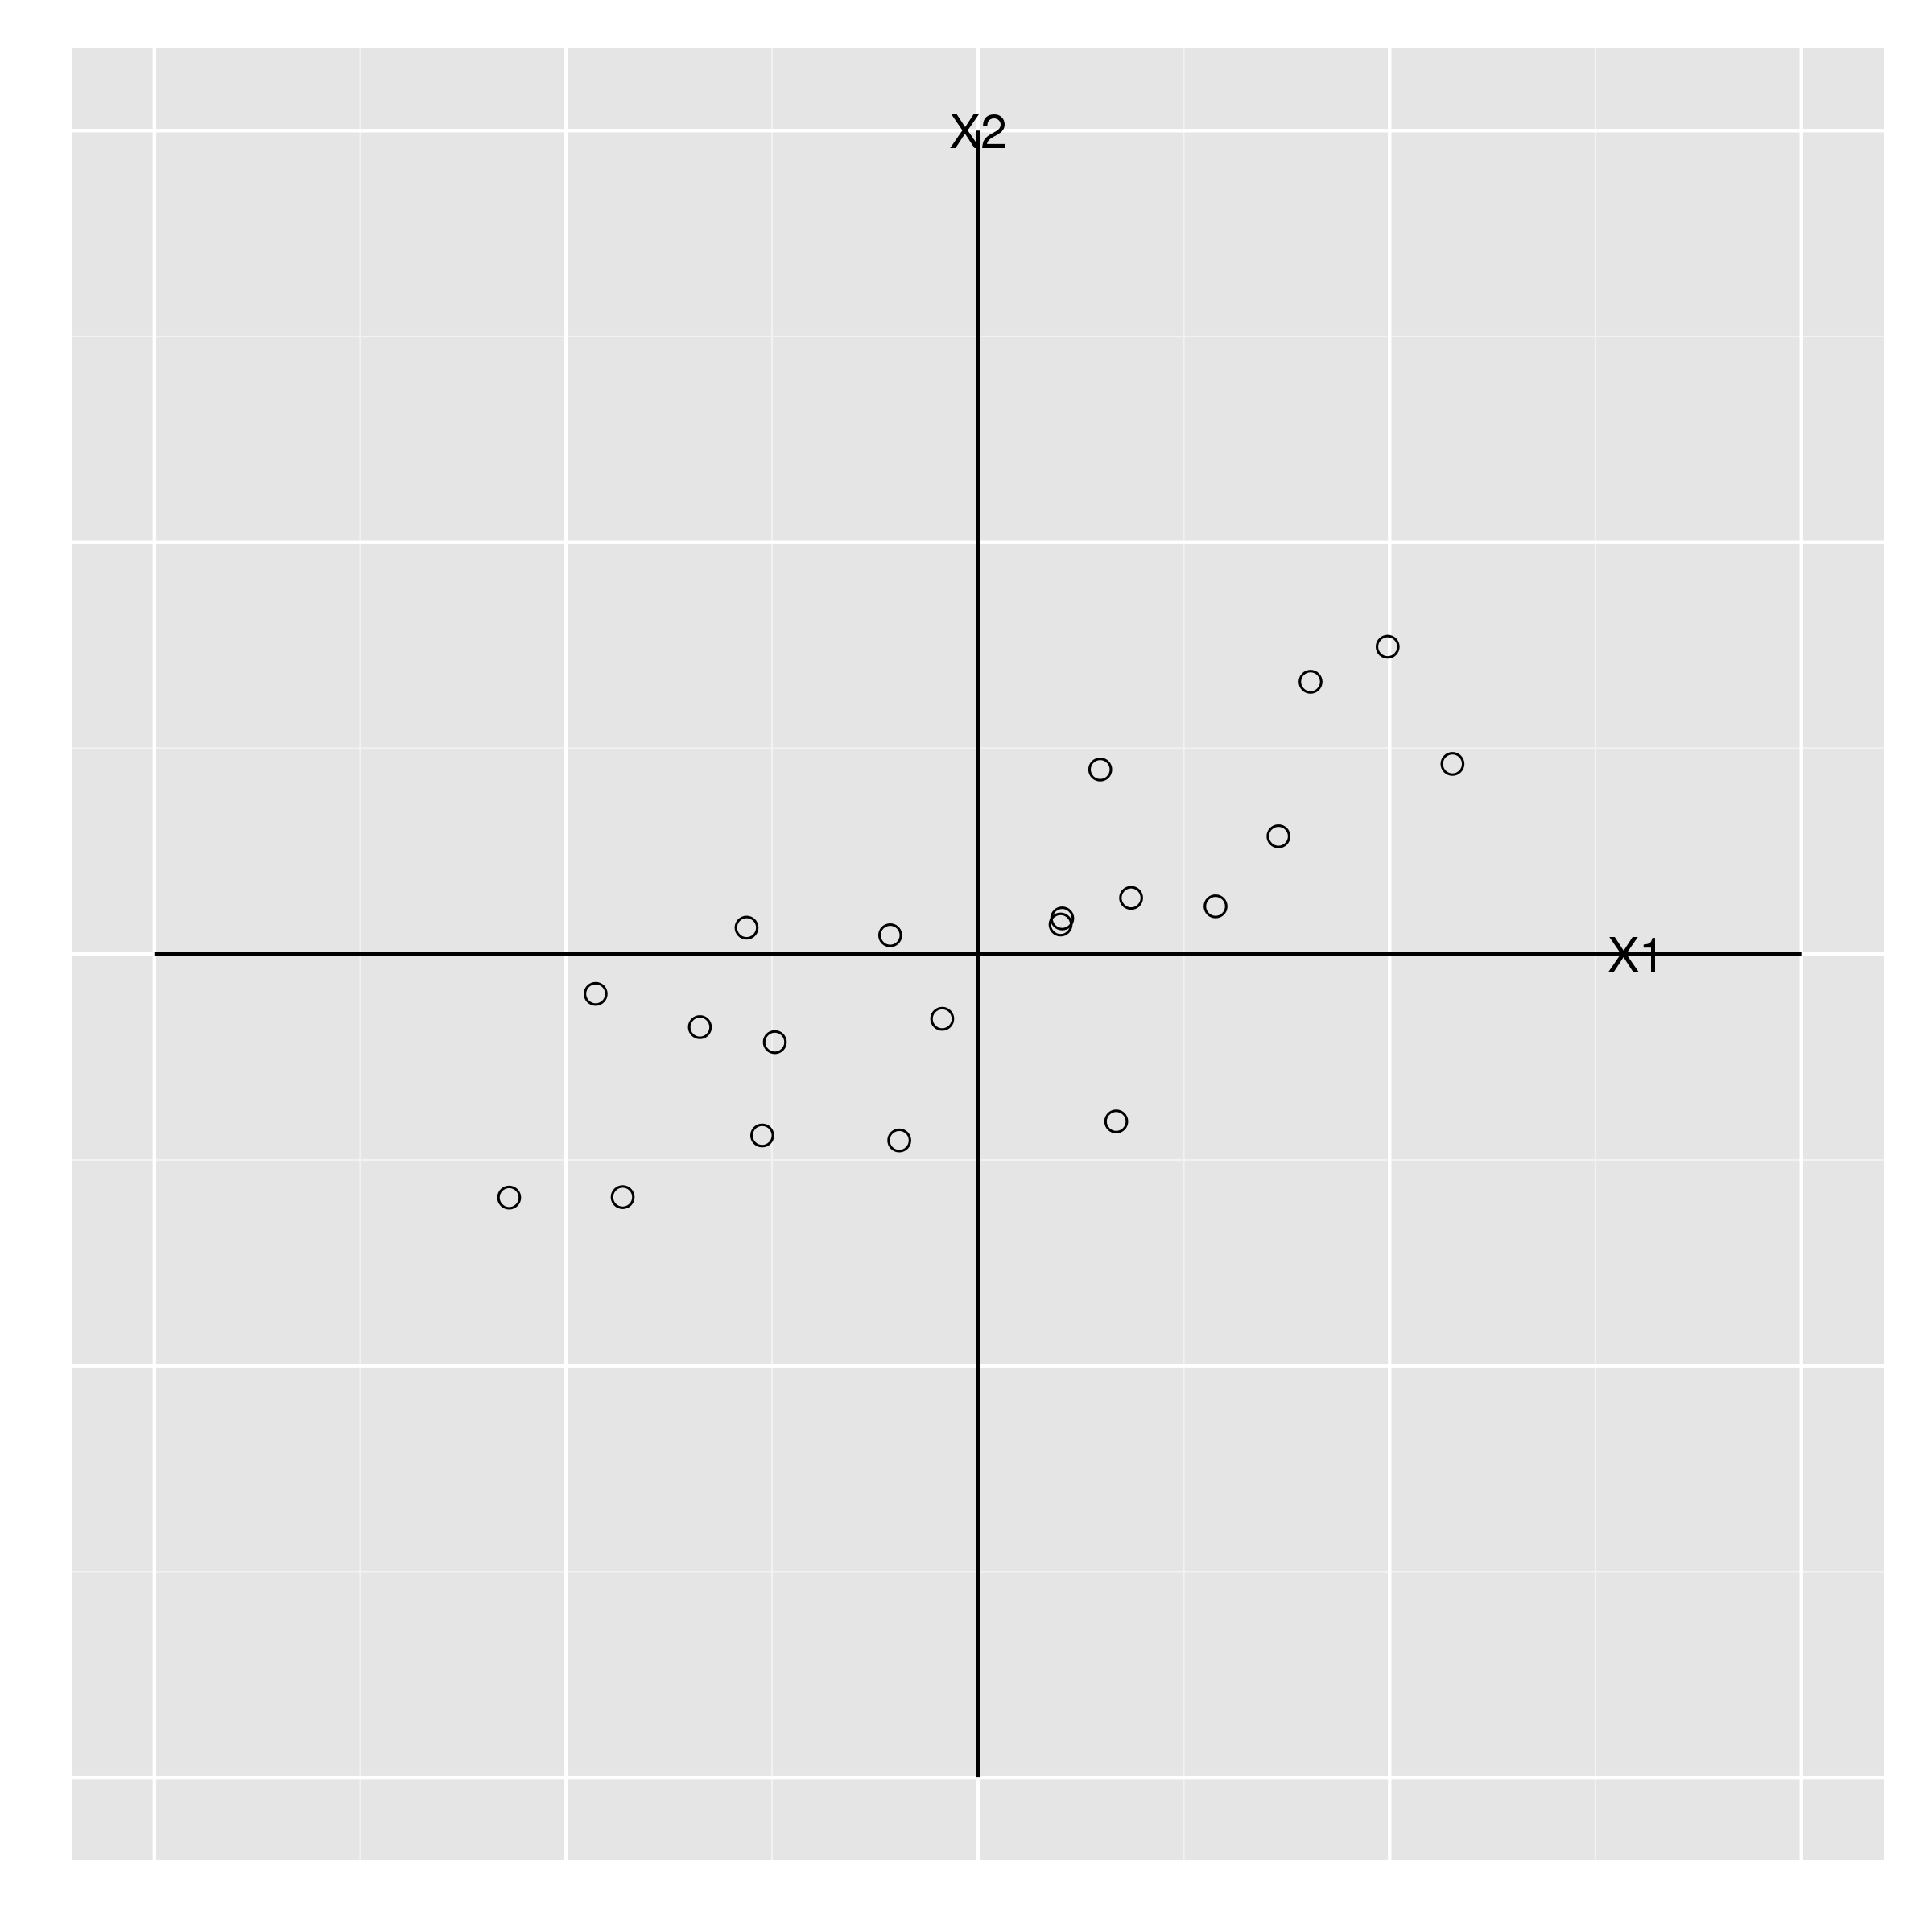
\includegraphics[height=7cm]{x1x2z1z2rotated00.png}
 \end{center}
   \end{overlayarea}
 \end{frame}
 
 \begin{frame}\frametitle{Cambio de sistema de coordenadas}
   \begin{overlayarea}{\textwidth}{8cm} 
 \begin{center}
   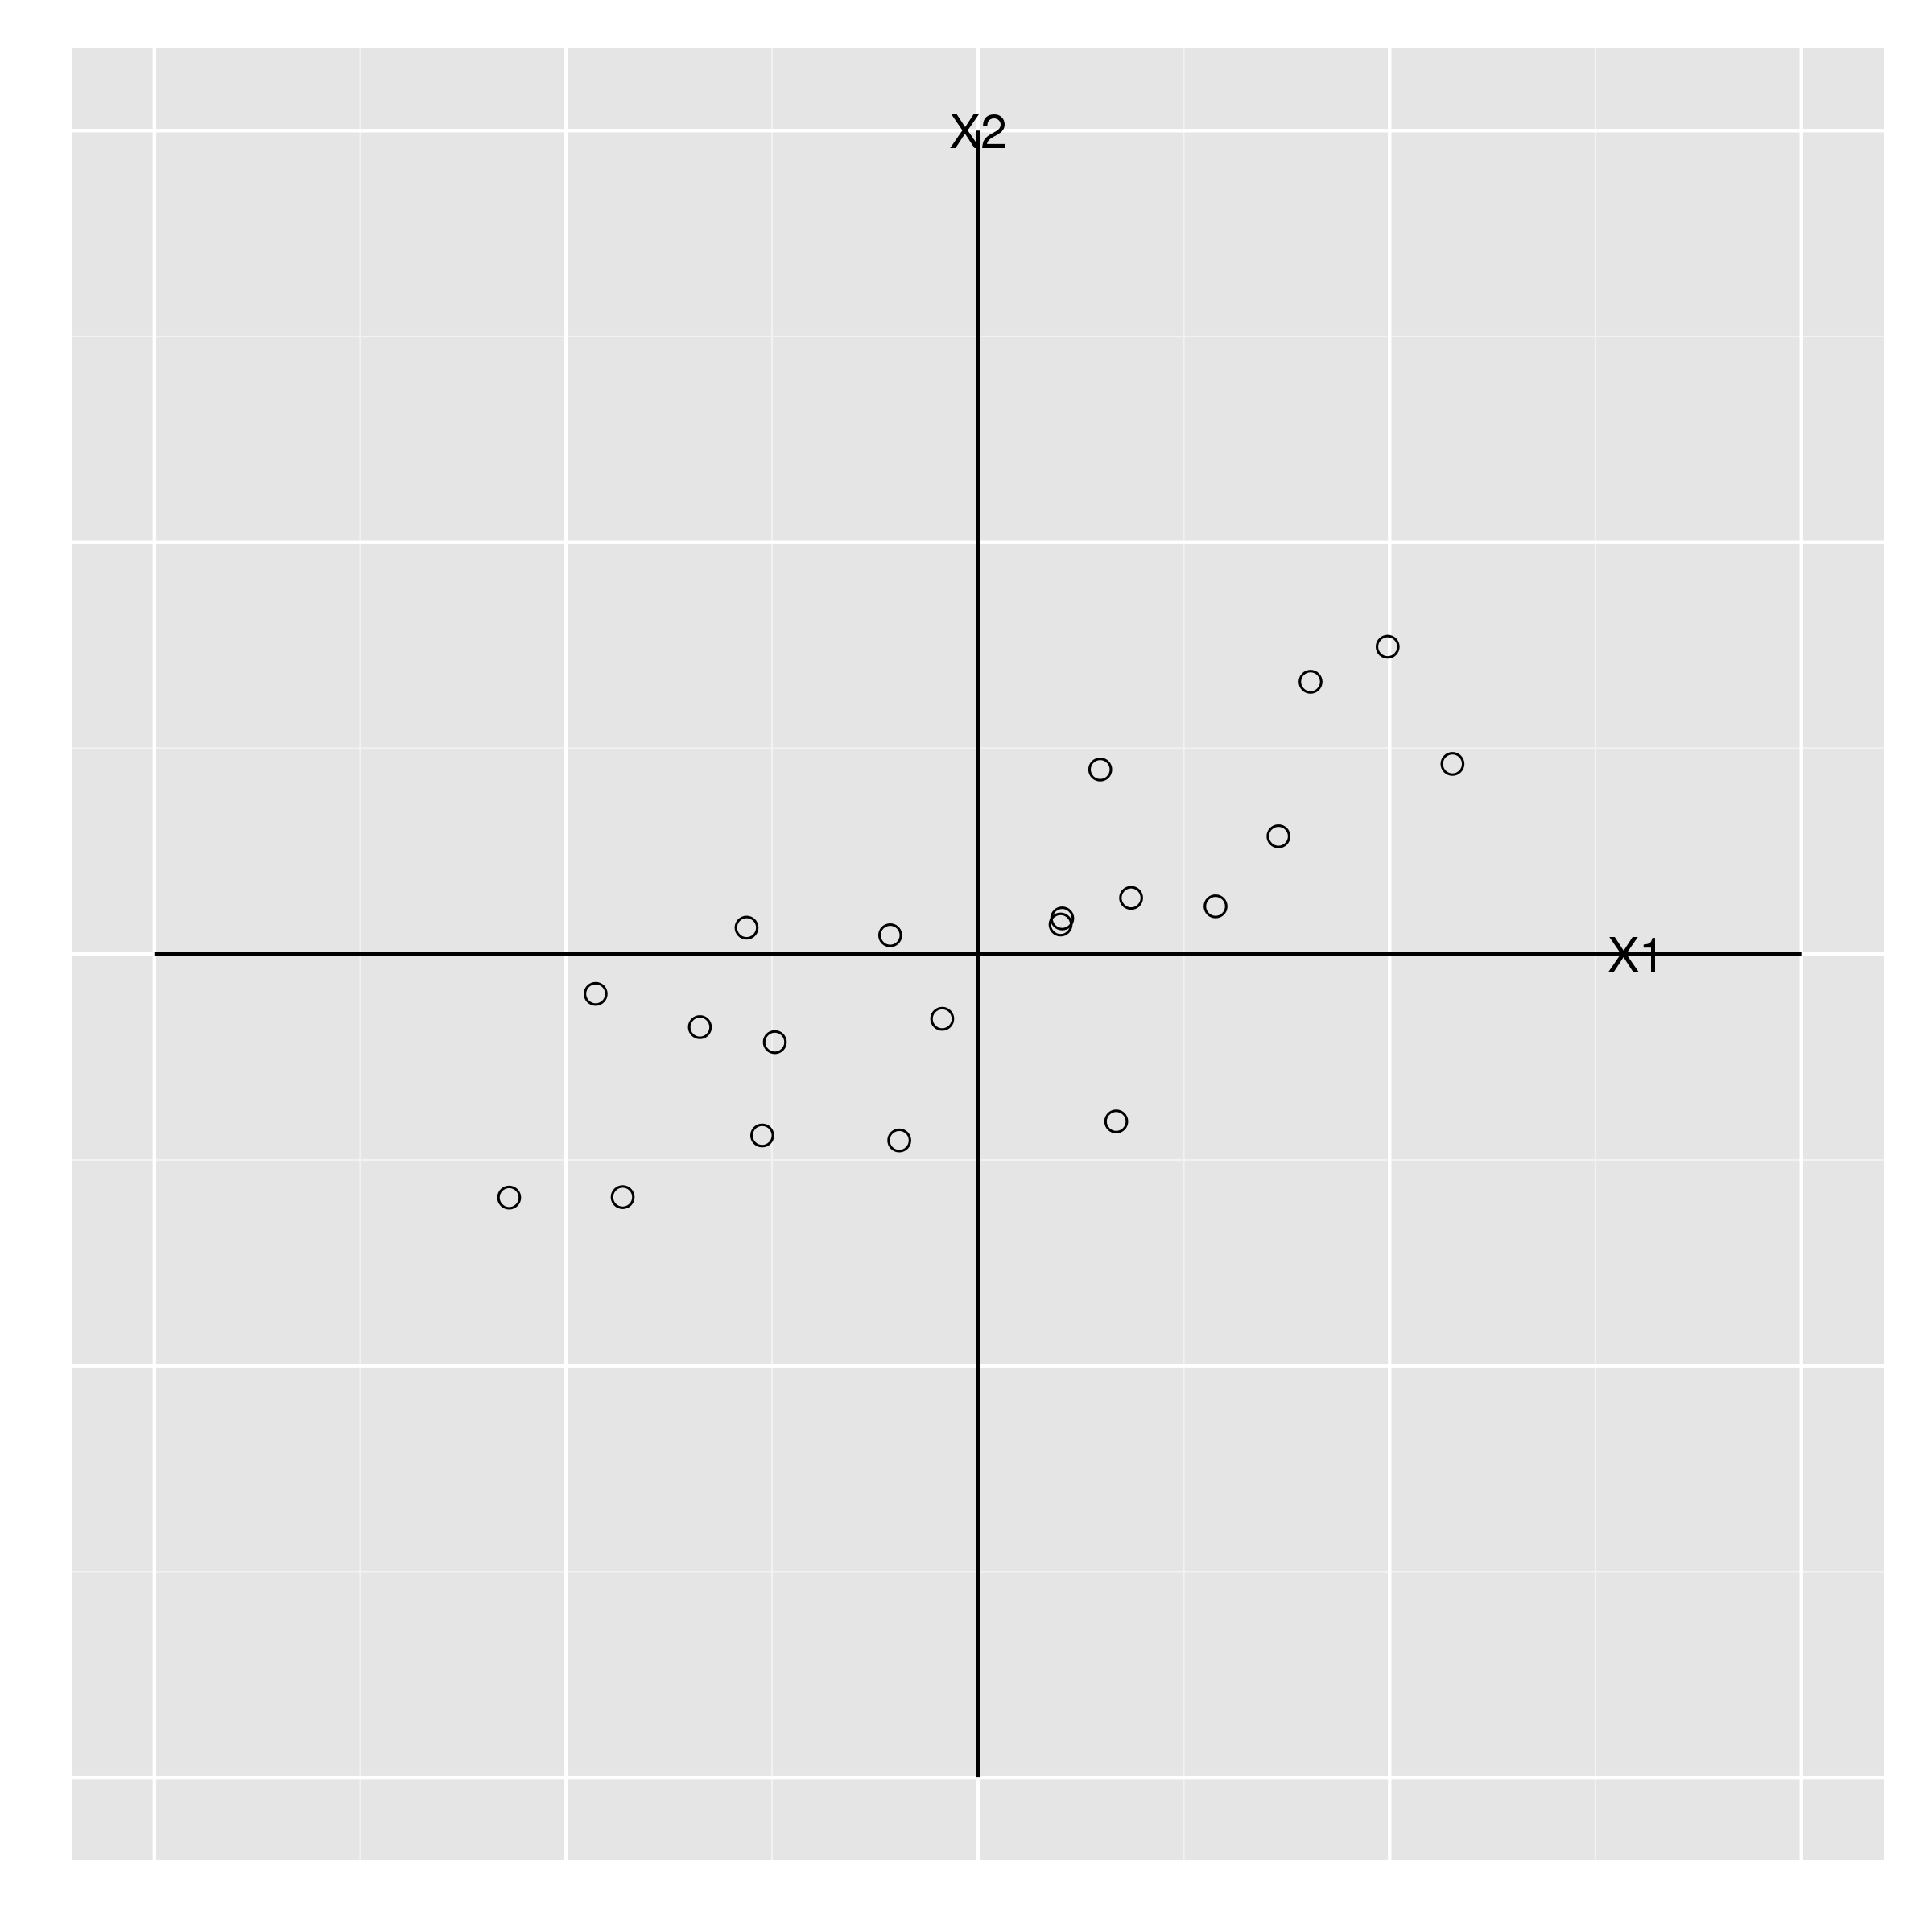
\includegraphics[height=7cm]{x1x2z1z2rotated00.png}
 \end{center}
   \end{overlayarea}
 \end{frame}
\begin{frame}\frametitle{Cambio de sistema de coordenadas}
   \begin{overlayarea}{\textwidth}{8cm} 
 \begin{center}
   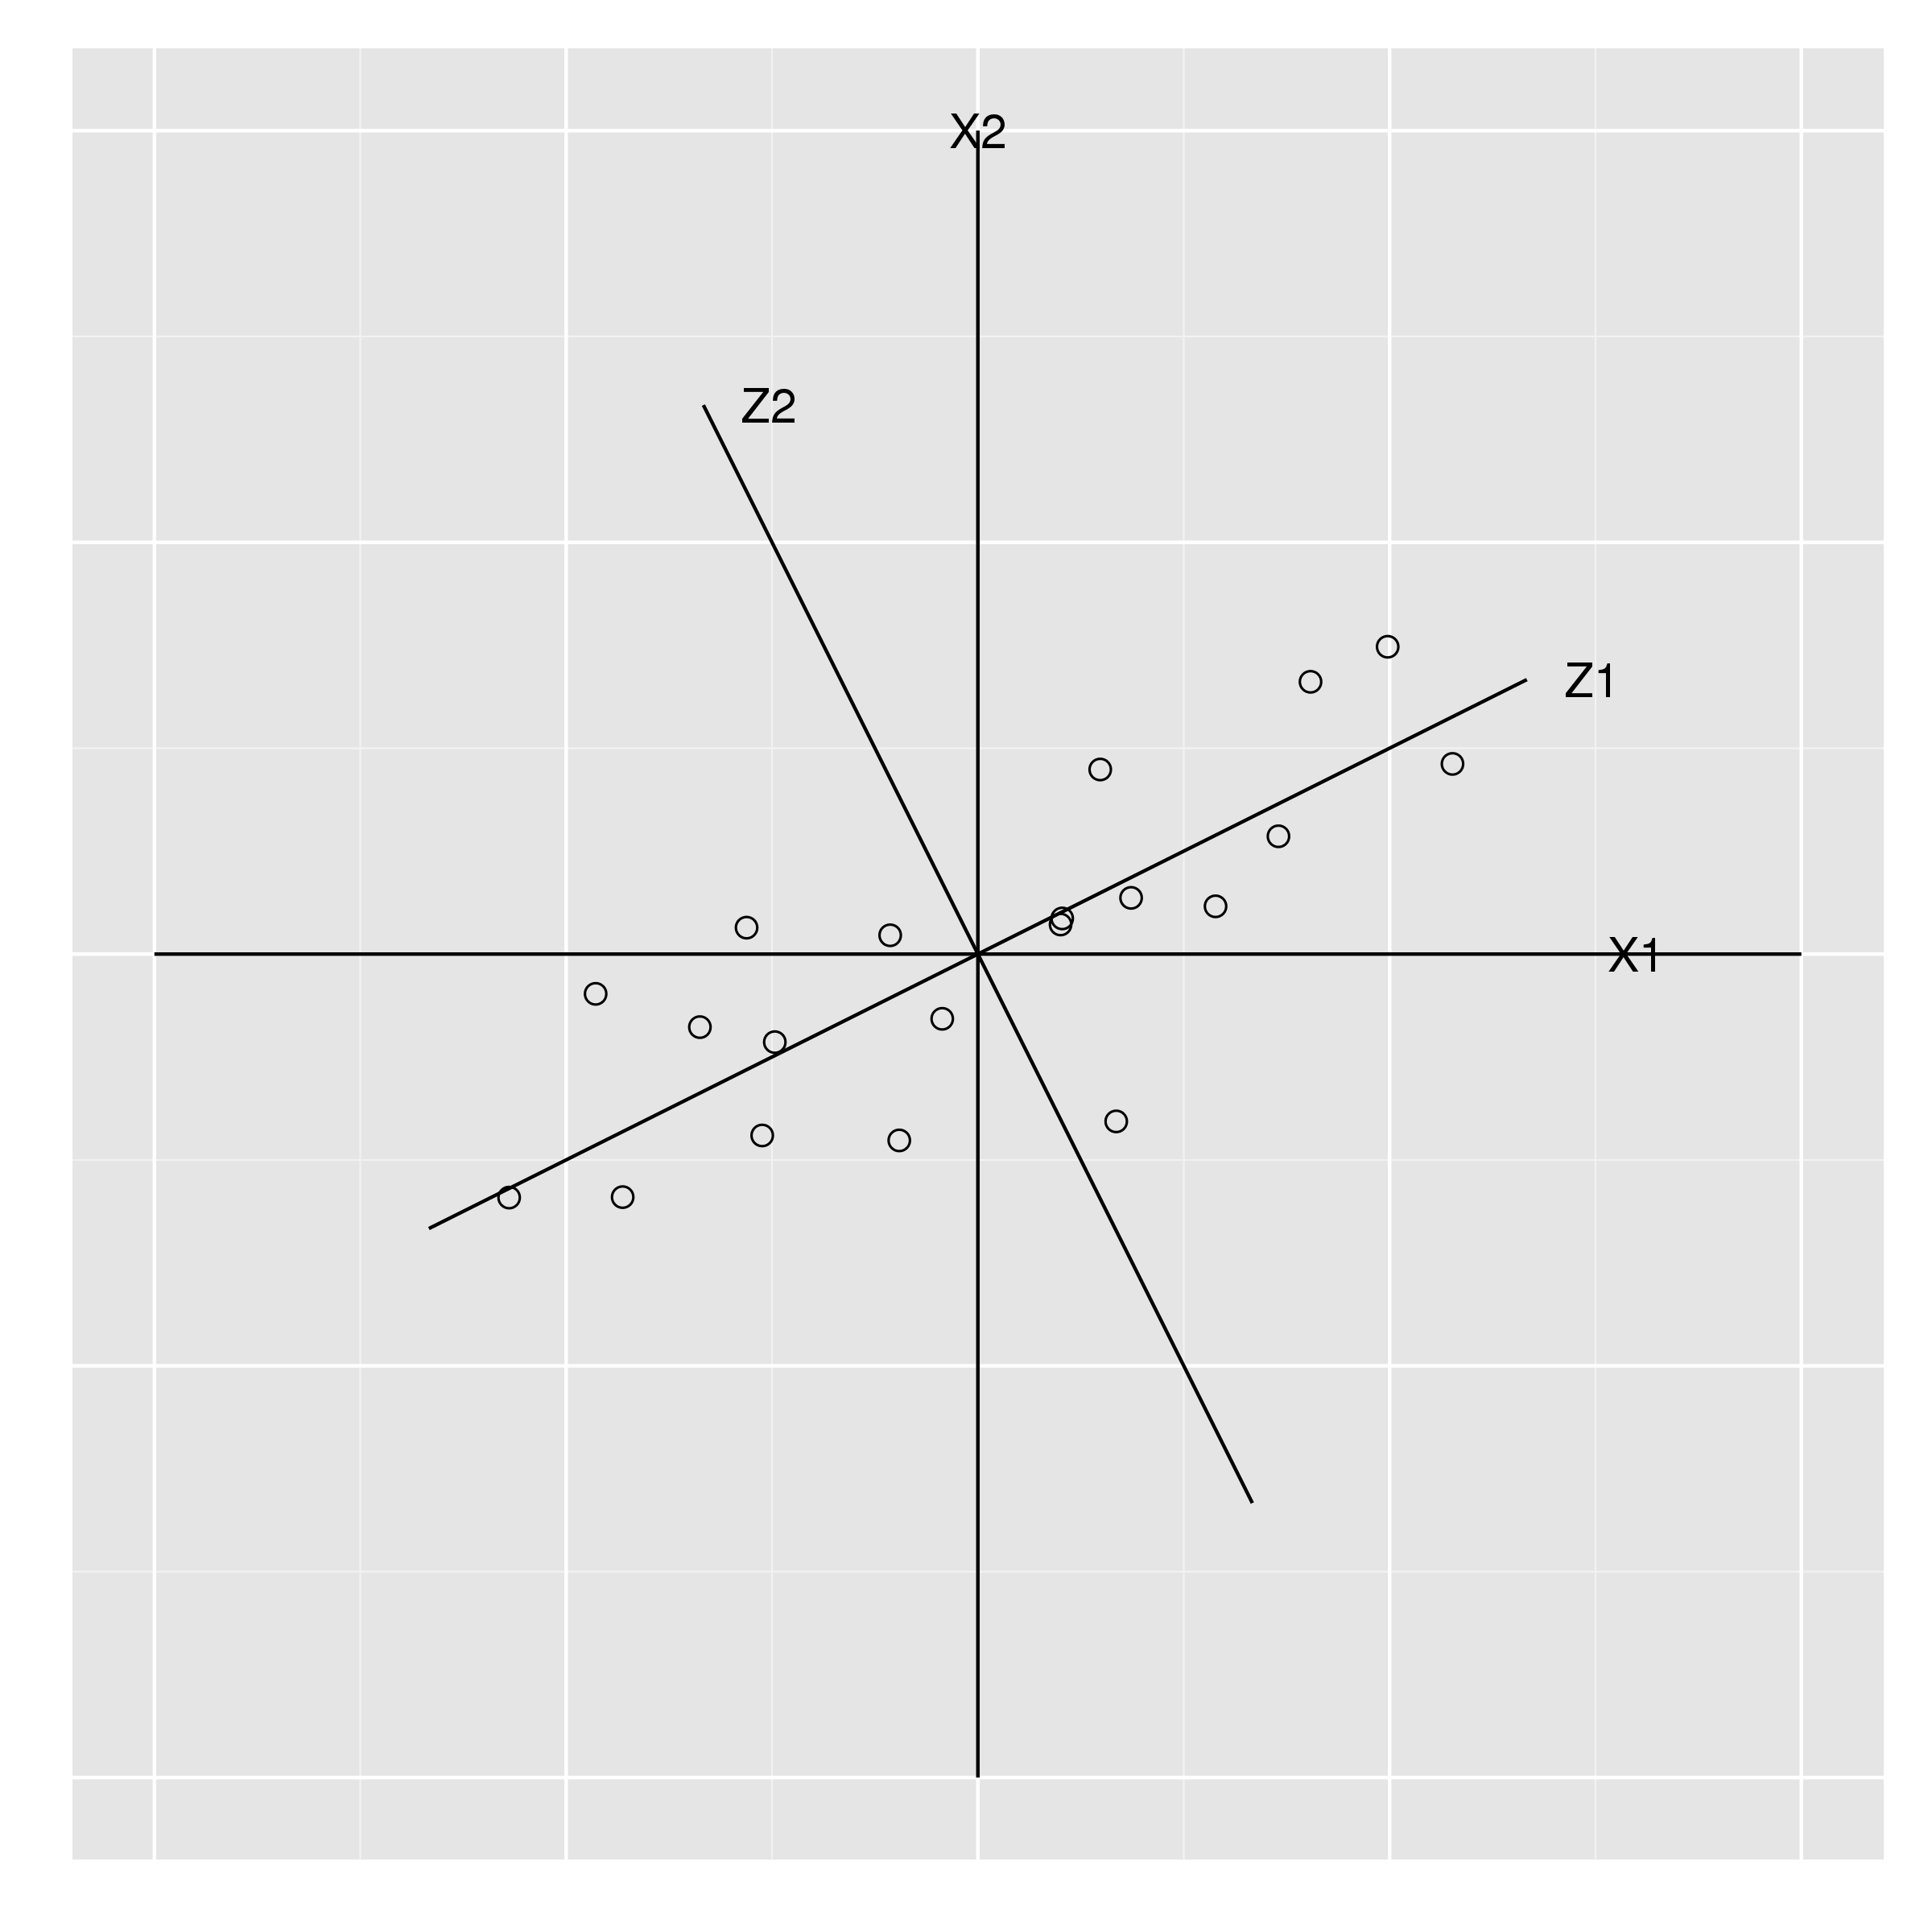
\includegraphics[height=7cm]{x1x2z1z2rotated01.png}
 \end{center}
   \end{overlayarea}
 \end{frame}
\begin{frame}\frametitle{Cambio de sistema de coordenadas}
  \transduration{0.05}
  \begin{overlayarea}{\textwidth}{8cm} 
 \begin{center}
   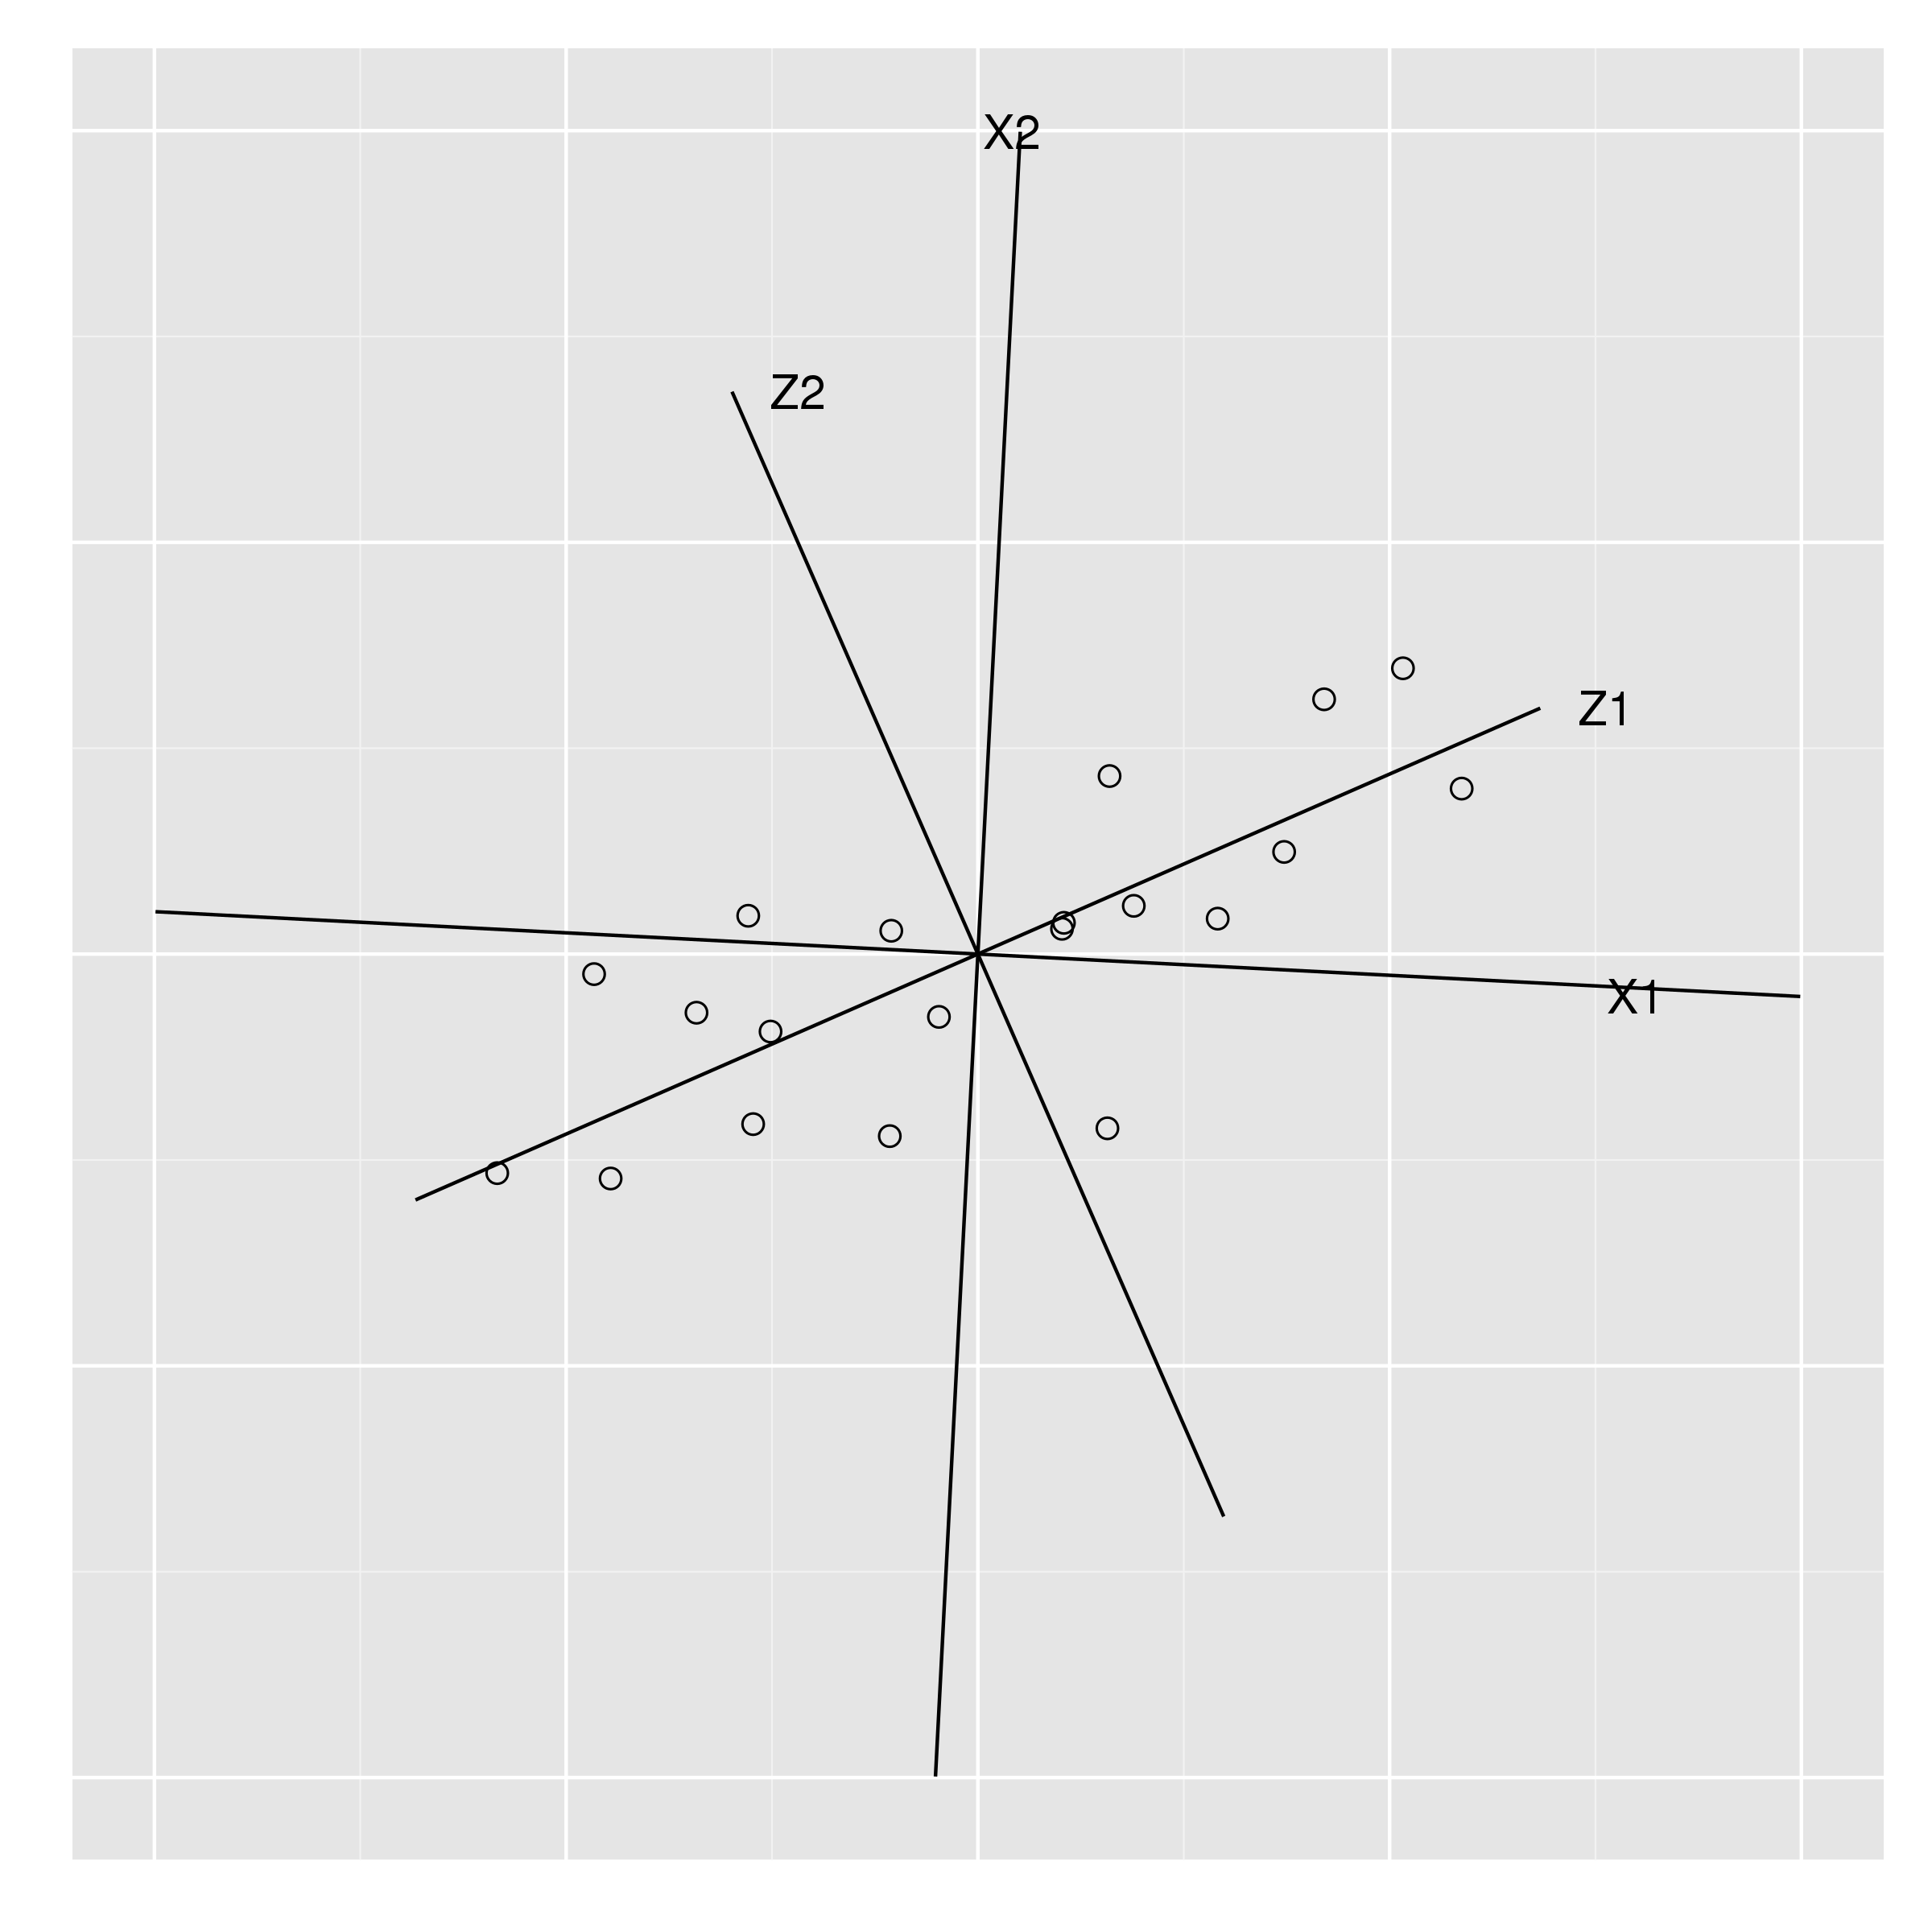
\includegraphics[height=7cm]{x1x2z1z2rotated02.png}
 \end{center}
   \end{overlayarea}
 \end{frame}
\begin{frame}\frametitle{Cambio de sistema de coordenadas}
  \transduration{0.05}
   \begin{overlayarea}{\textwidth}{8cm} 
 \begin{center}
   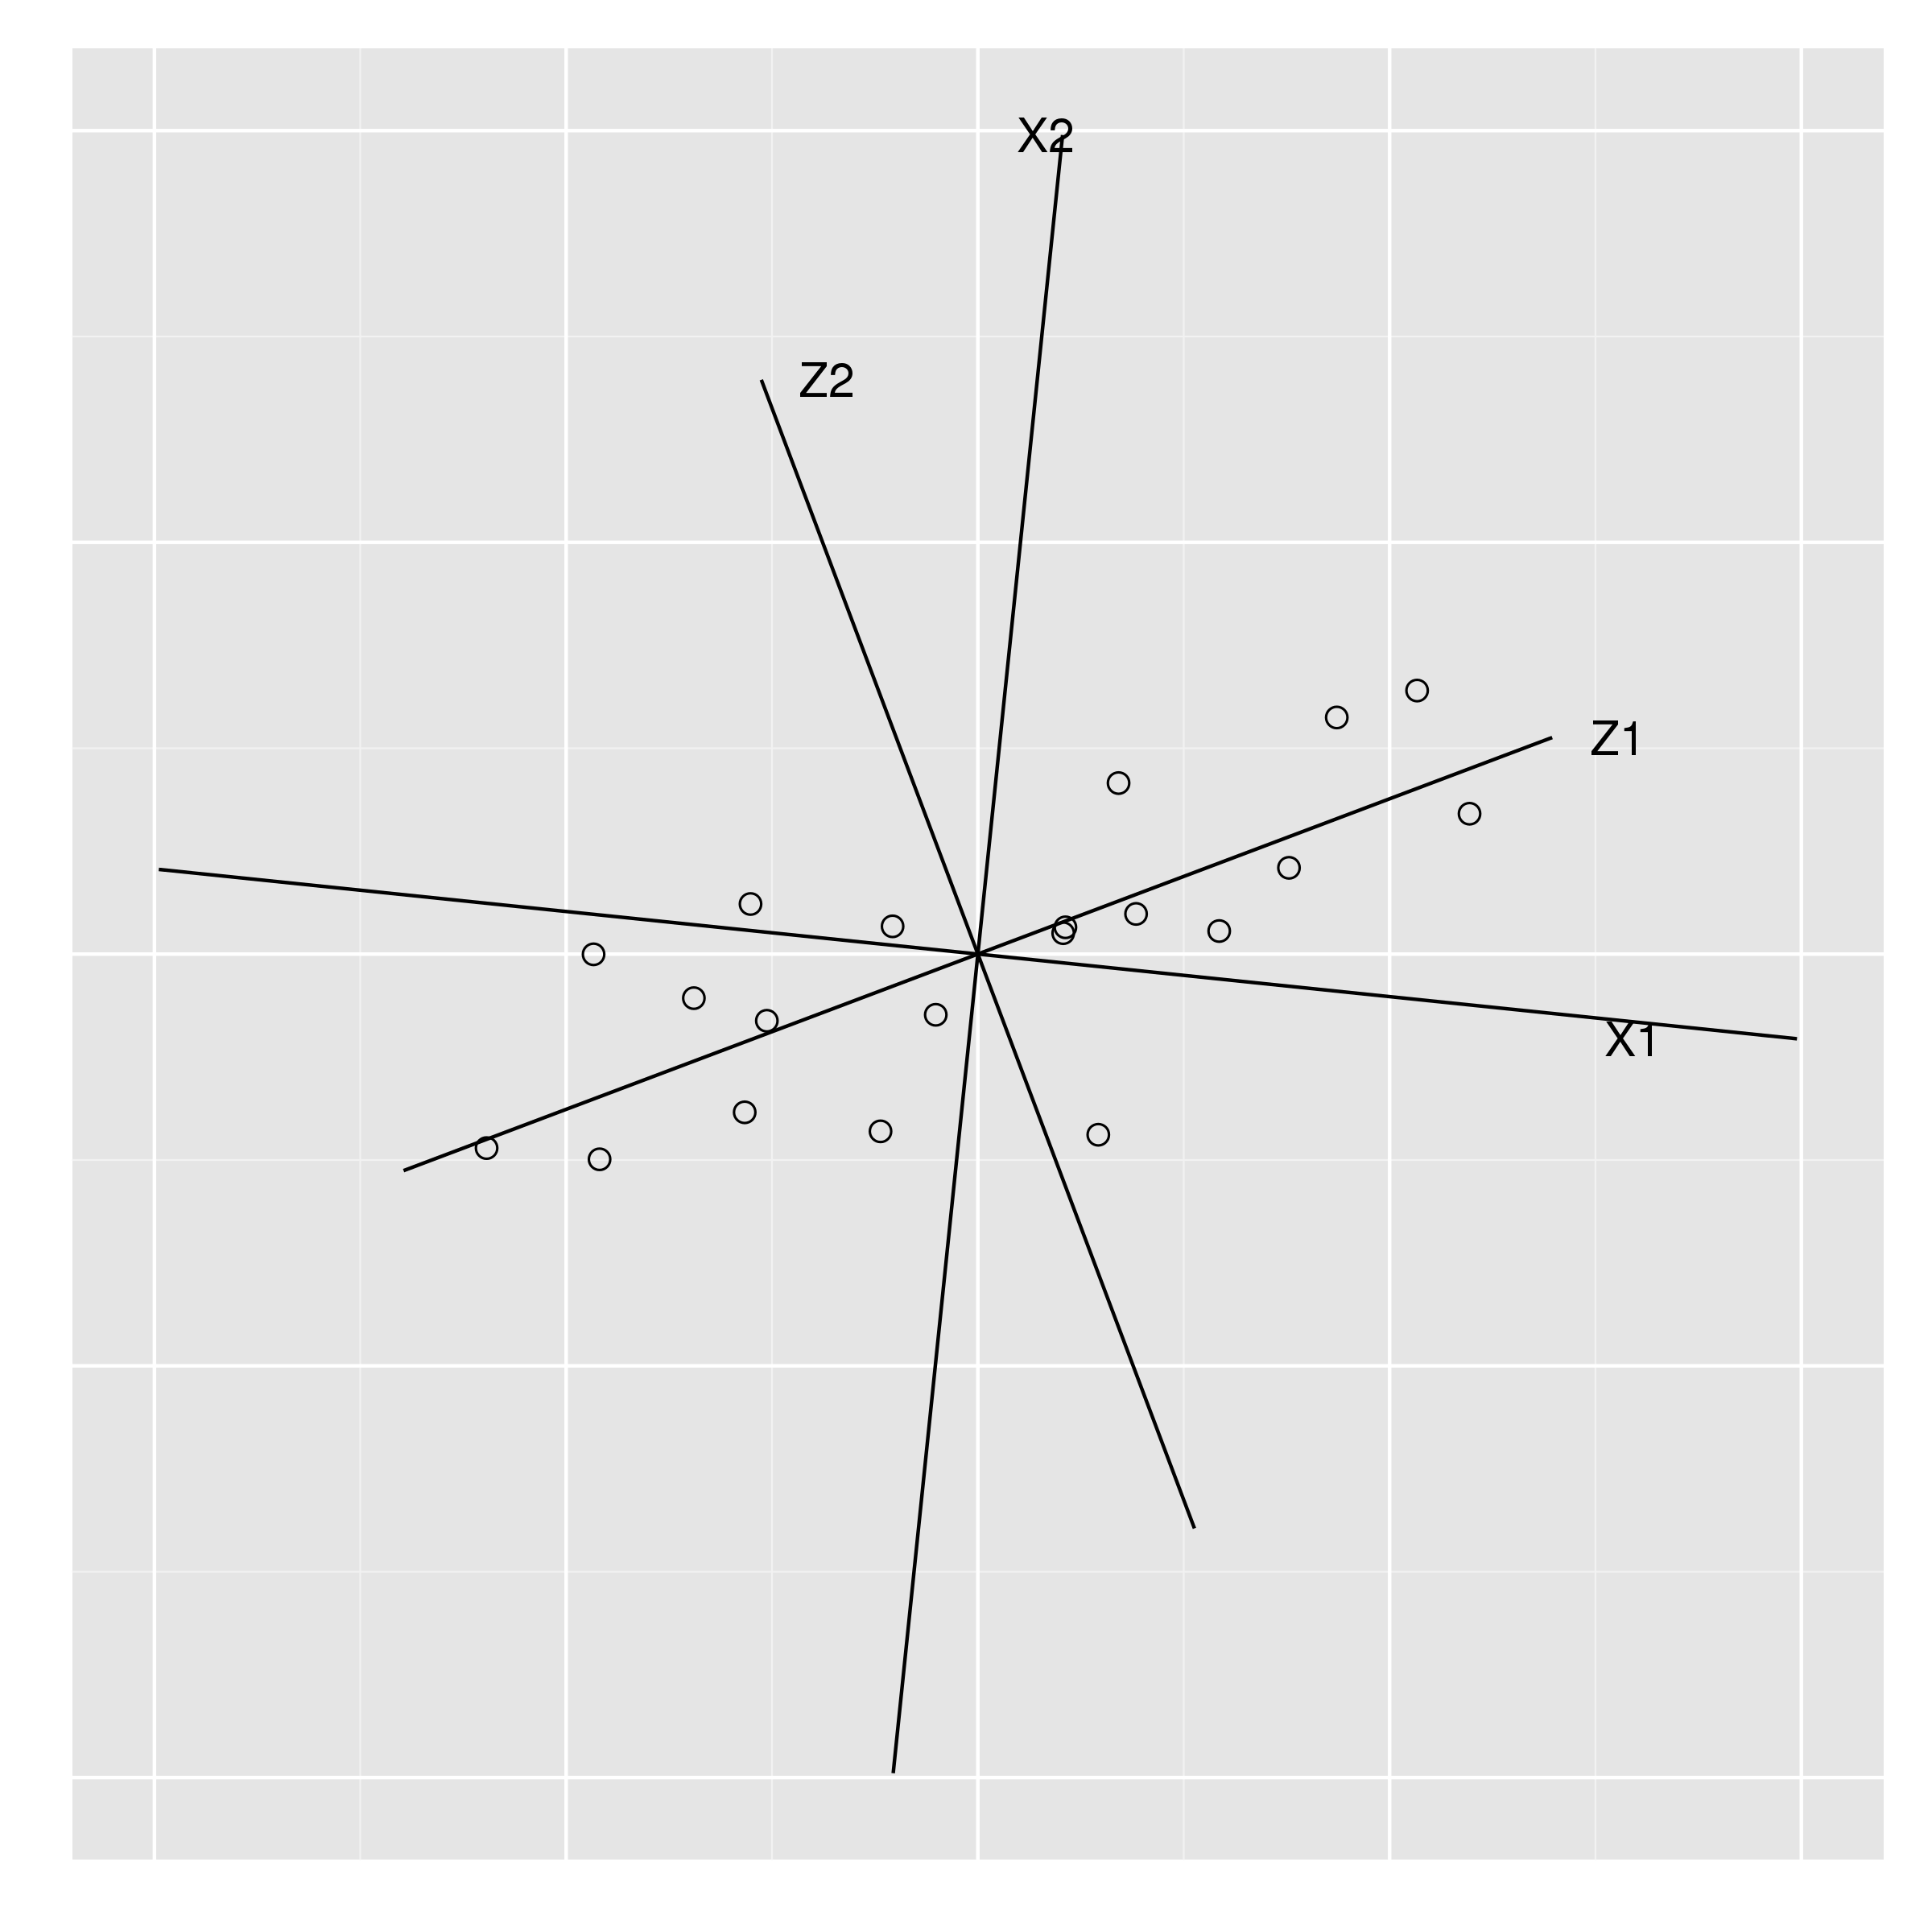
\includegraphics[height=7cm]{x1x2z1z2rotated03.png}
 \end{center}
   \end{overlayarea}
 \end{frame}
\begin{frame}\frametitle{Cambio de sistema de coordenadas}
  \transduration{0.05}
   \begin{overlayarea}{\textwidth}{8cm} 
 \begin{center}
   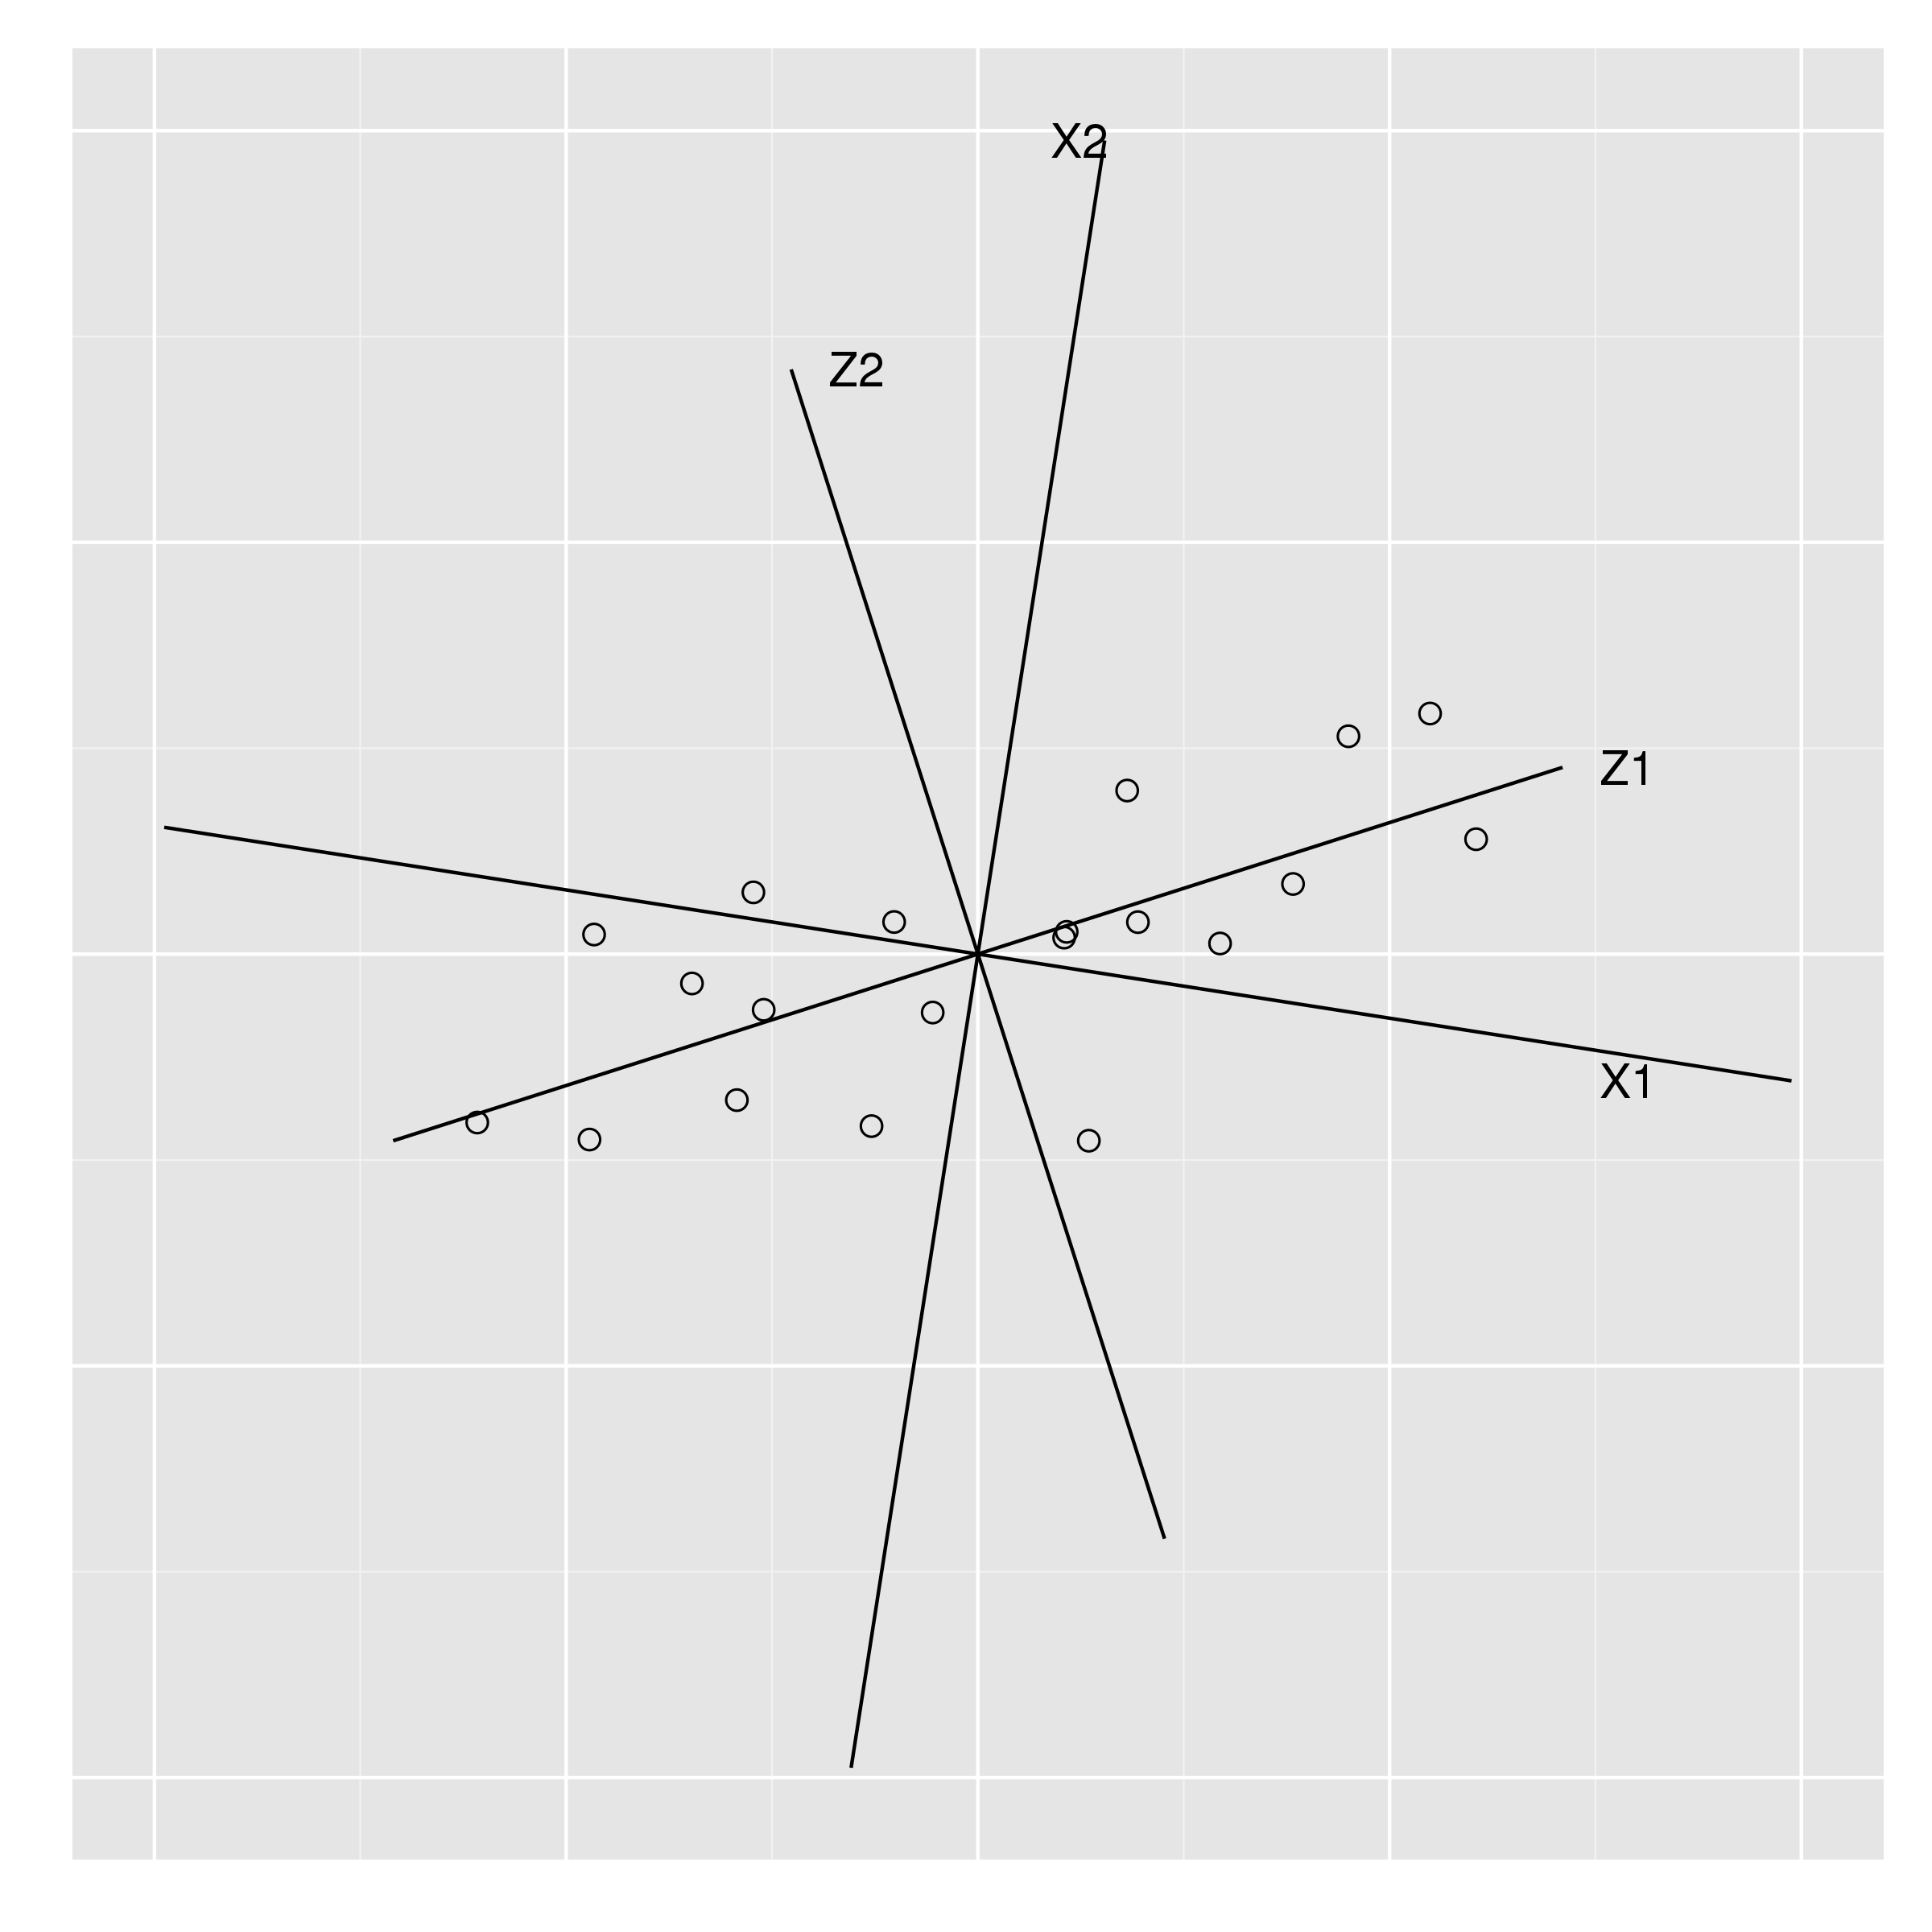
\includegraphics[height=7cm]{x1x2z1z2rotated04.png}
 \end{center}
   \end{overlayarea}
 \end{frame}
\begin{frame}\frametitle{Cambio de sistema de coordenadas}
  \transduration{0.05}
   \begin{overlayarea}{\textwidth}{8cm} 
 \begin{center}
   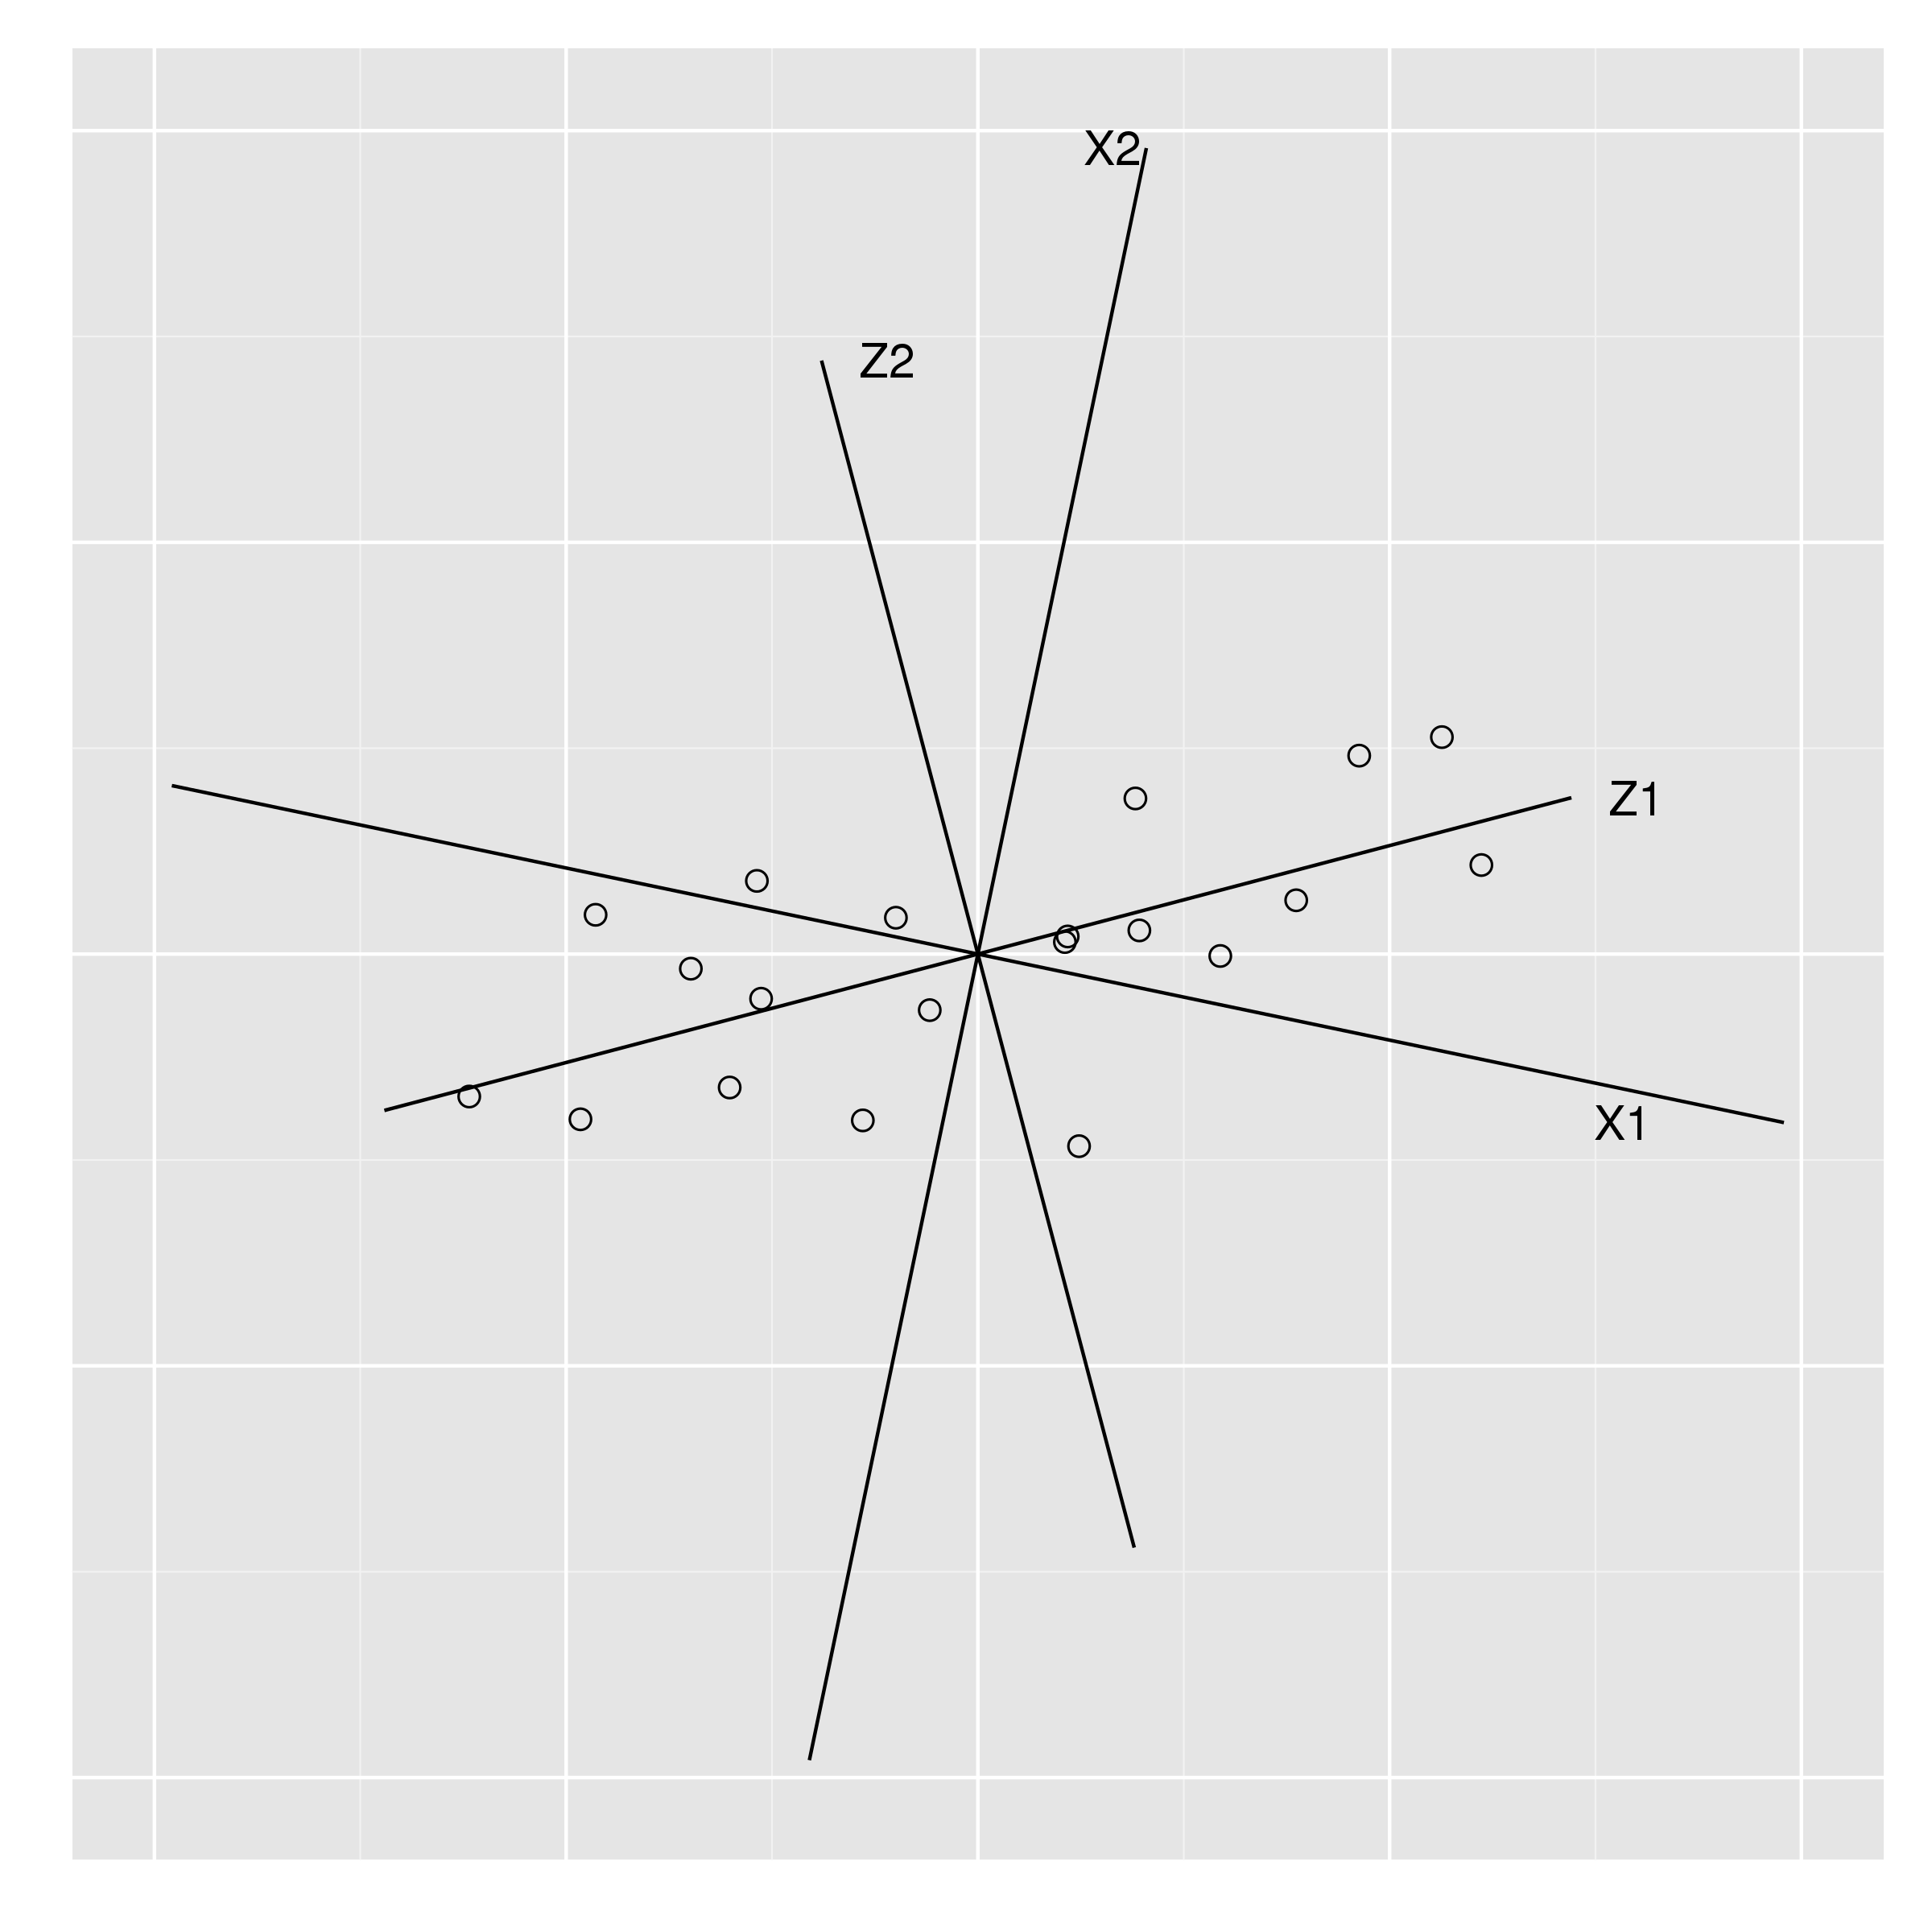
\includegraphics[height=7cm]{x1x2z1z2rotated05.png}
 \end{center}
   \end{overlayarea}
 \end{frame}
\begin{frame}\frametitle{Cambio de sistema de coordenadas}
  \transduration{0.05}
   \begin{overlayarea}{\textwidth}{8cm} 
 \begin{center}
   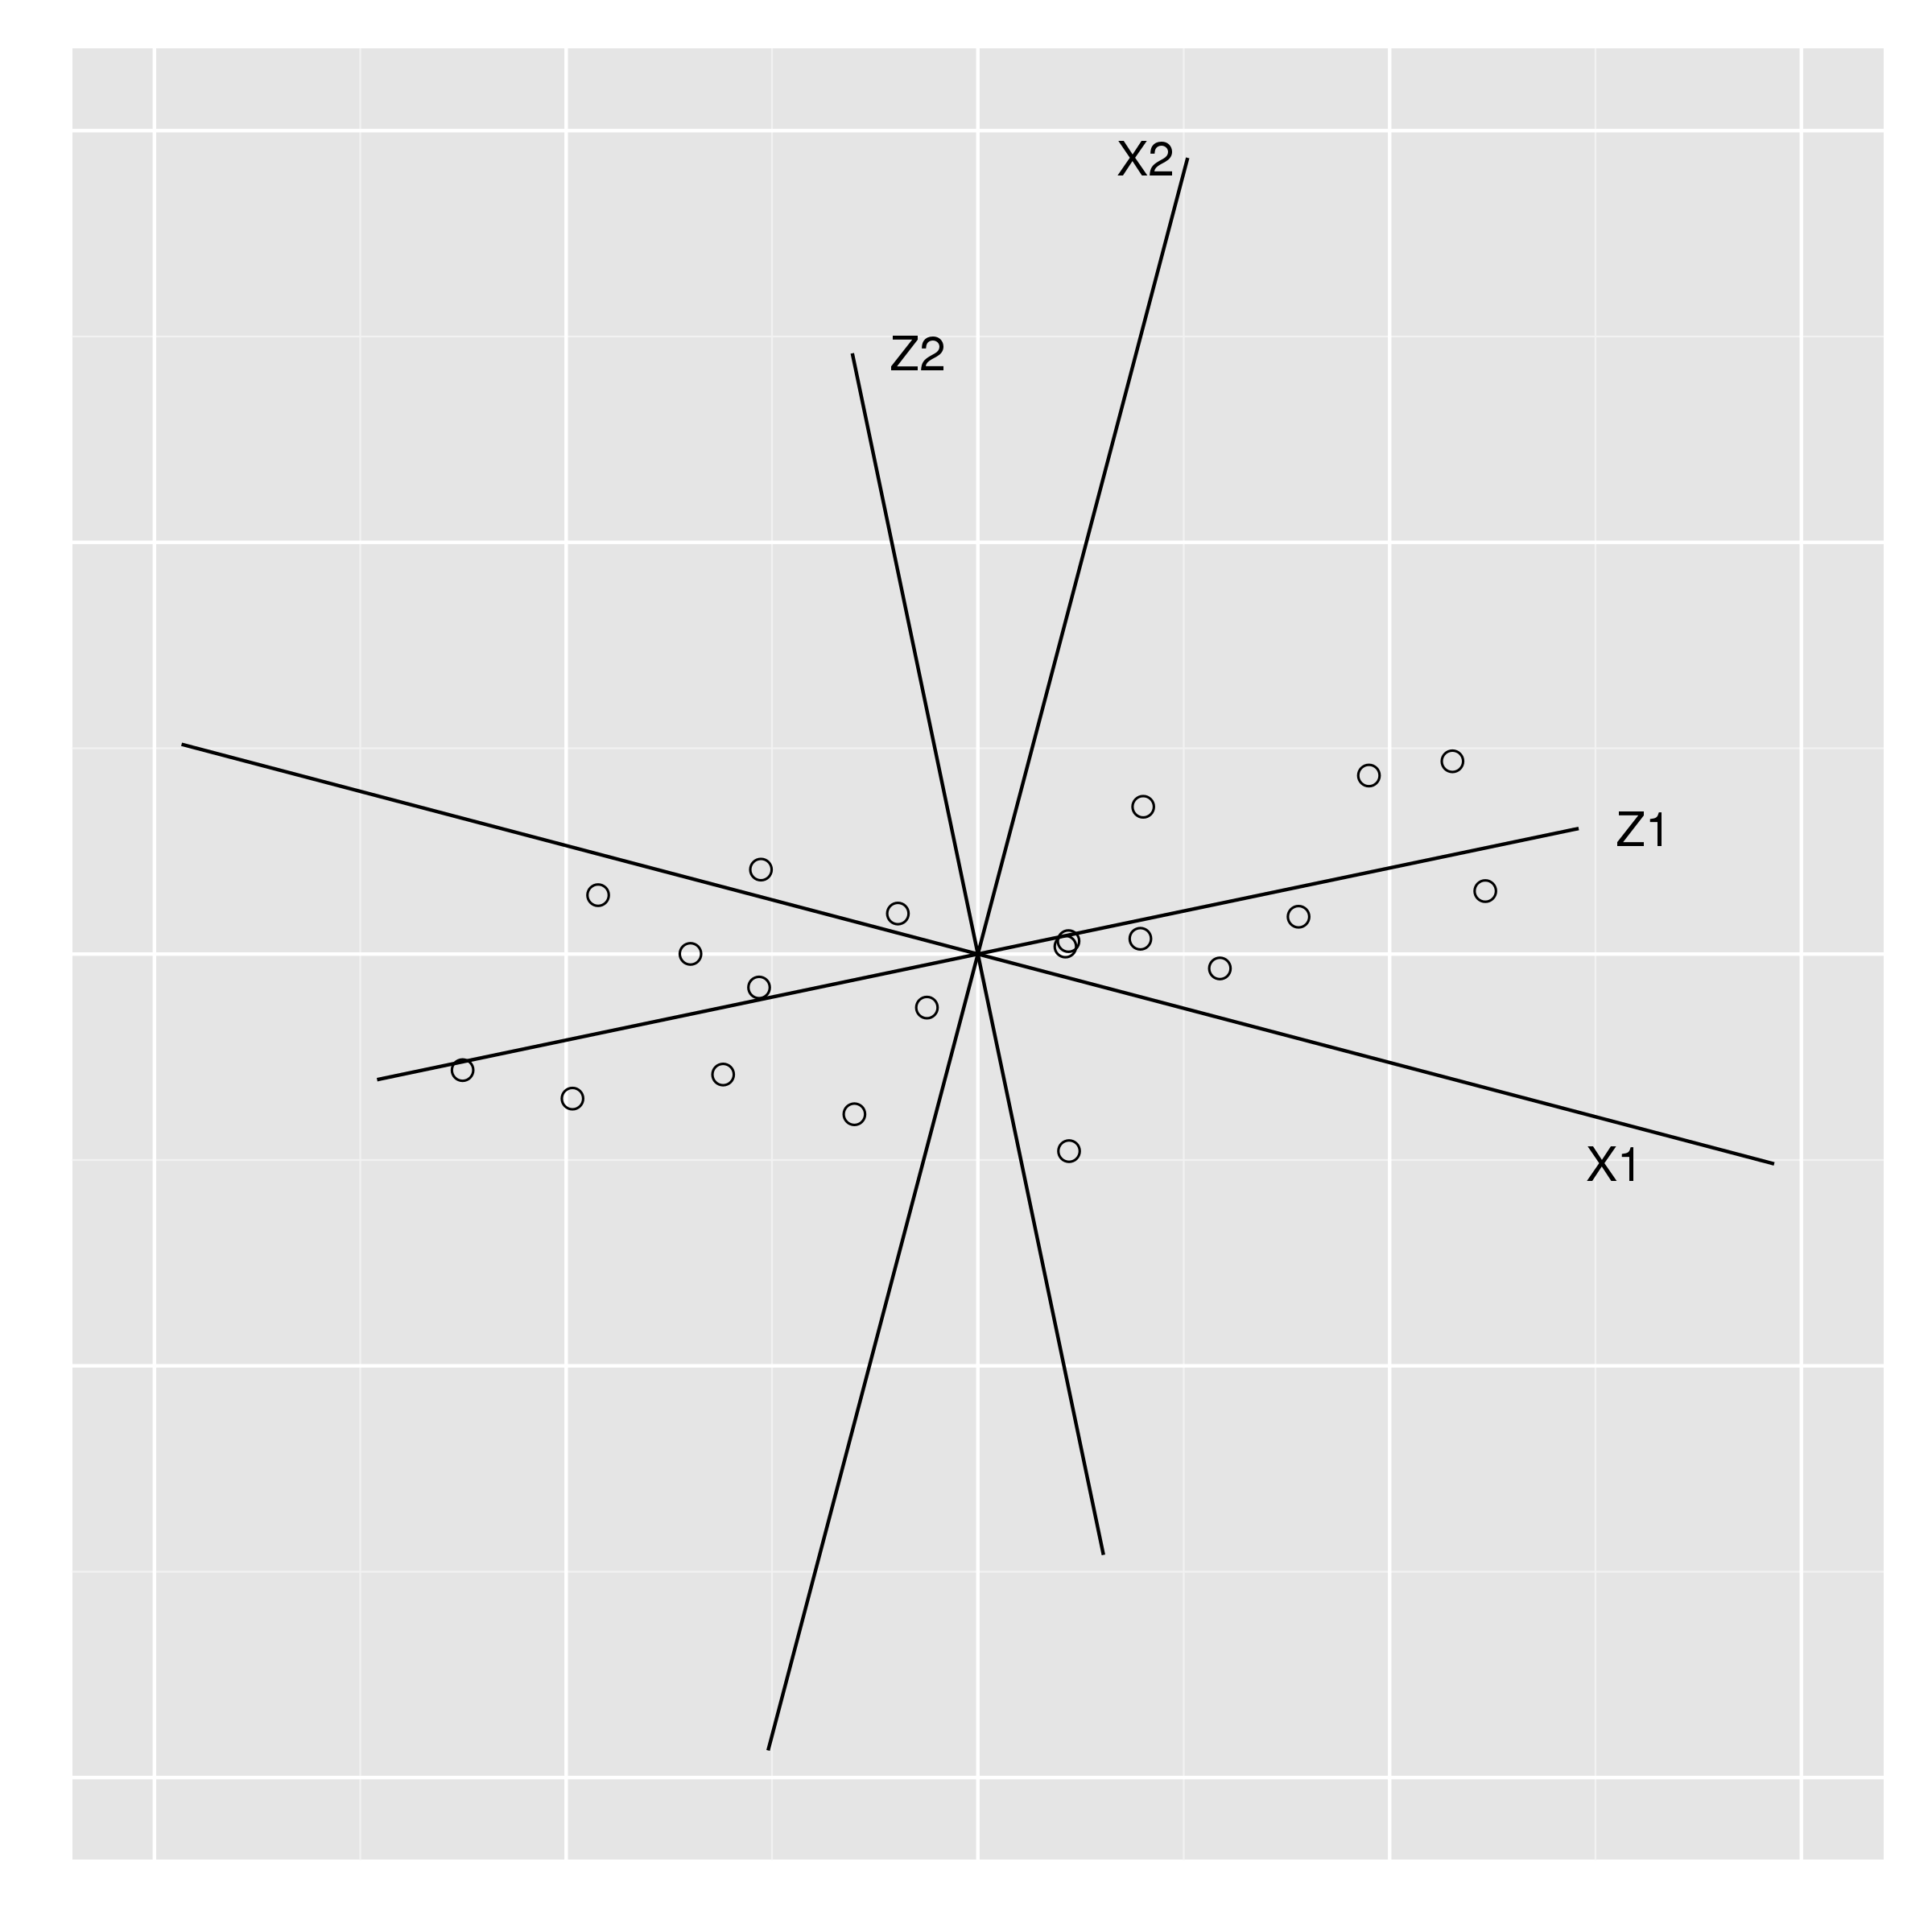
\includegraphics[height=7cm]{x1x2z1z2rotated06.png}
 \end{center}
   \end{overlayarea}
 \end{frame}
\begin{frame}\frametitle{Cambio de sistema de coordenadas}
  \transduration{0.05}
   \begin{overlayarea}{\textwidth}{8cm} 
 \begin{center}
   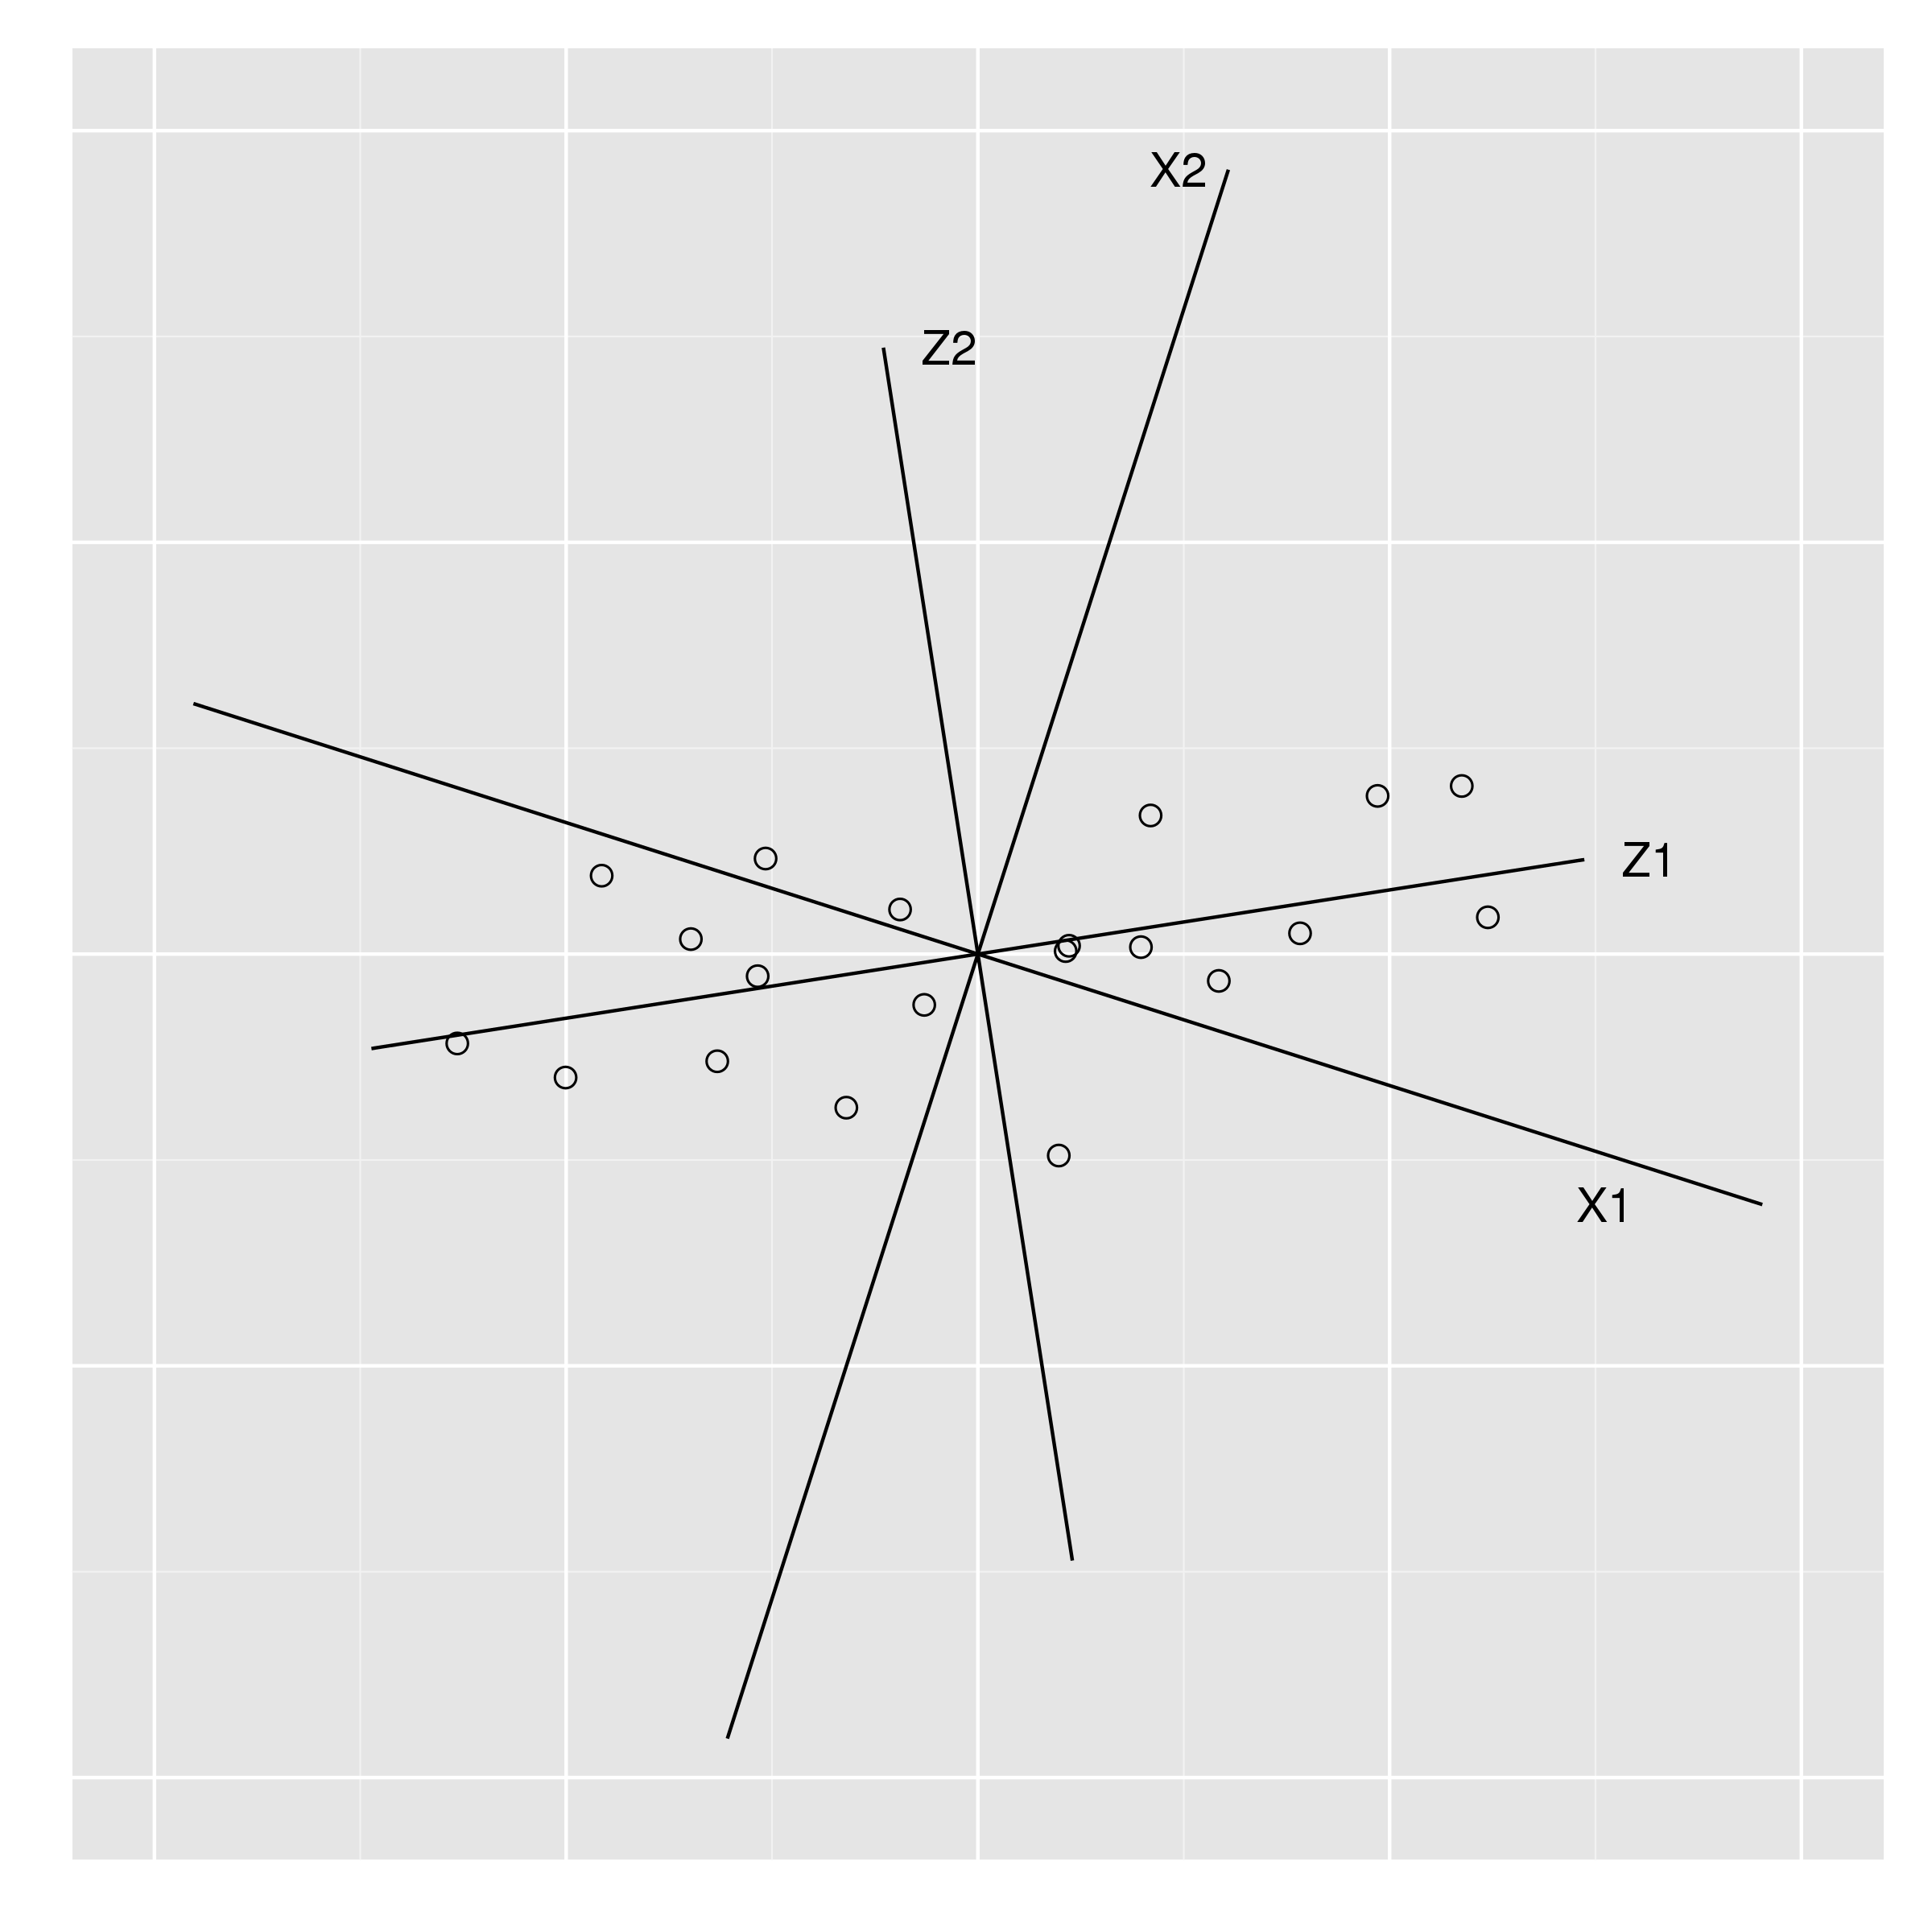
\includegraphics[height=7cm]{x1x2z1z2rotated07.png}
 \end{center}
   \end{overlayarea}
 \end{frame}
\begin{frame}\frametitle{Cambio de sistema de coordenadas}
  \transduration{0.05}
   \begin{overlayarea}{\textwidth}{8cm} 
 \begin{center}
   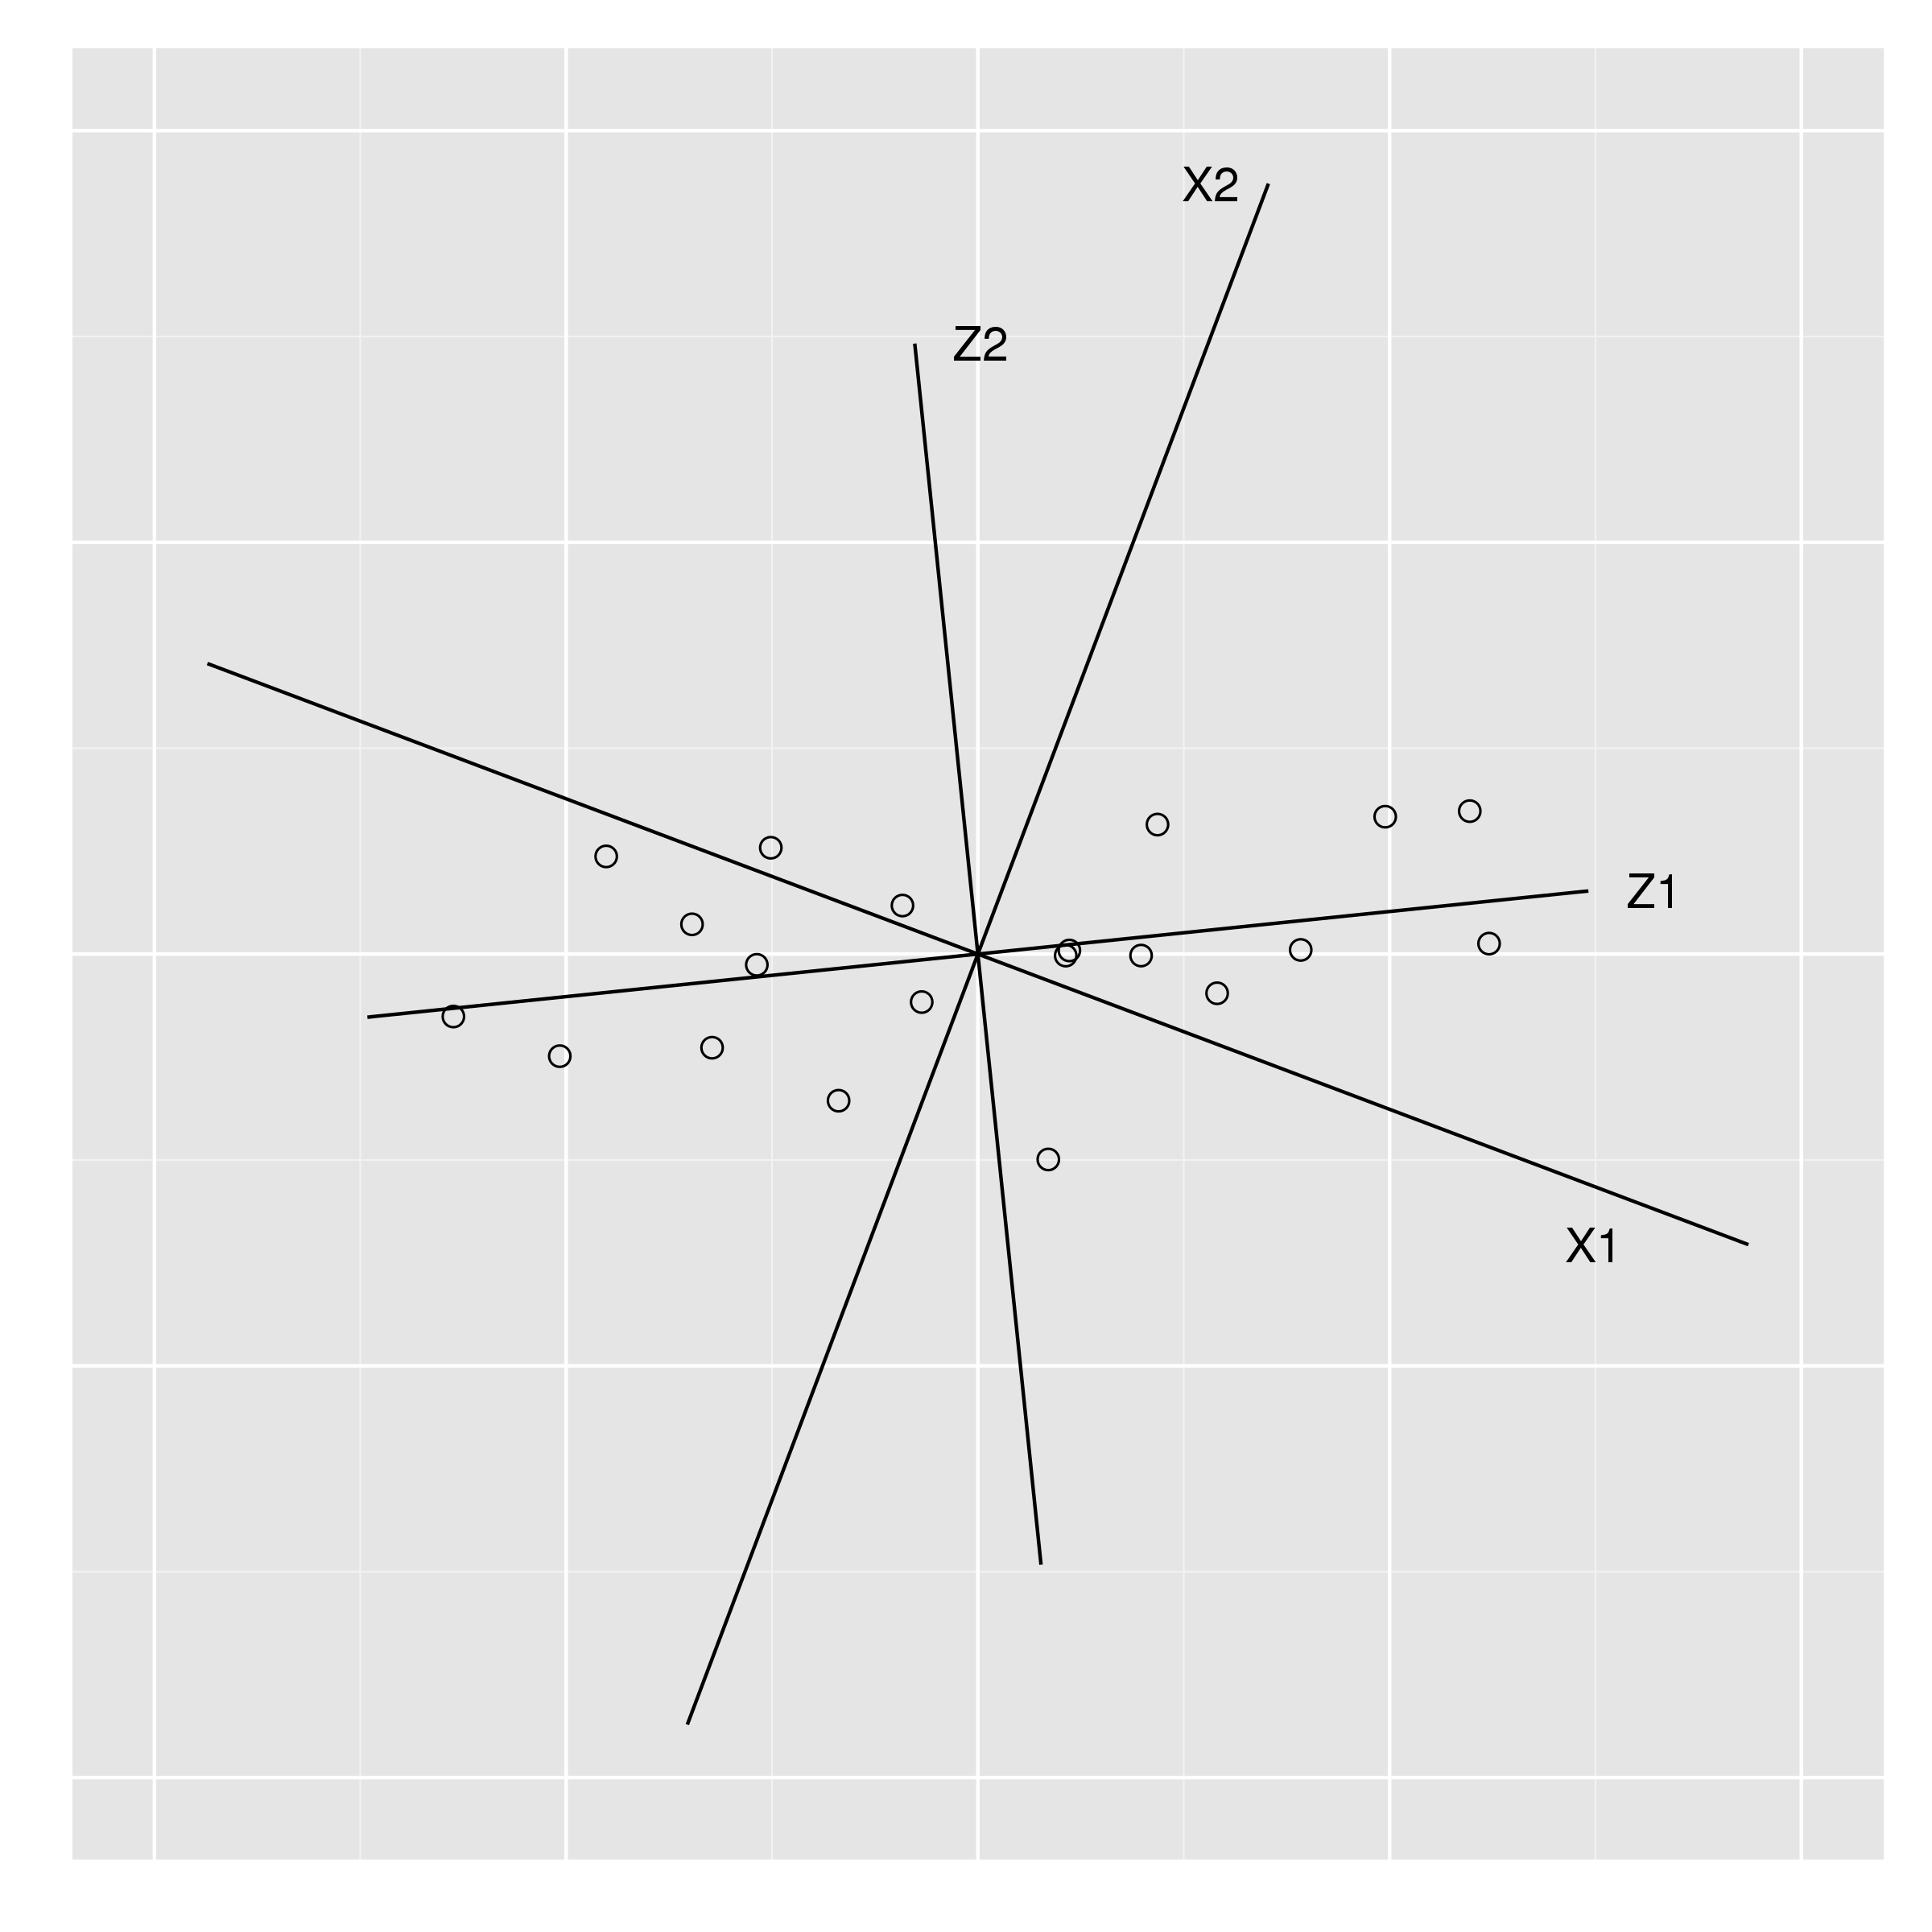
\includegraphics[height=7cm]{x1x2z1z2rotated08.png}
 \end{center}
   \end{overlayarea}
 \end{frame}
\begin{frame}\frametitle{Cambio de sistema de coordenadas}
  \transduration{0.05}
   \begin{overlayarea}{\textwidth}{8cm} 
 \begin{center}
   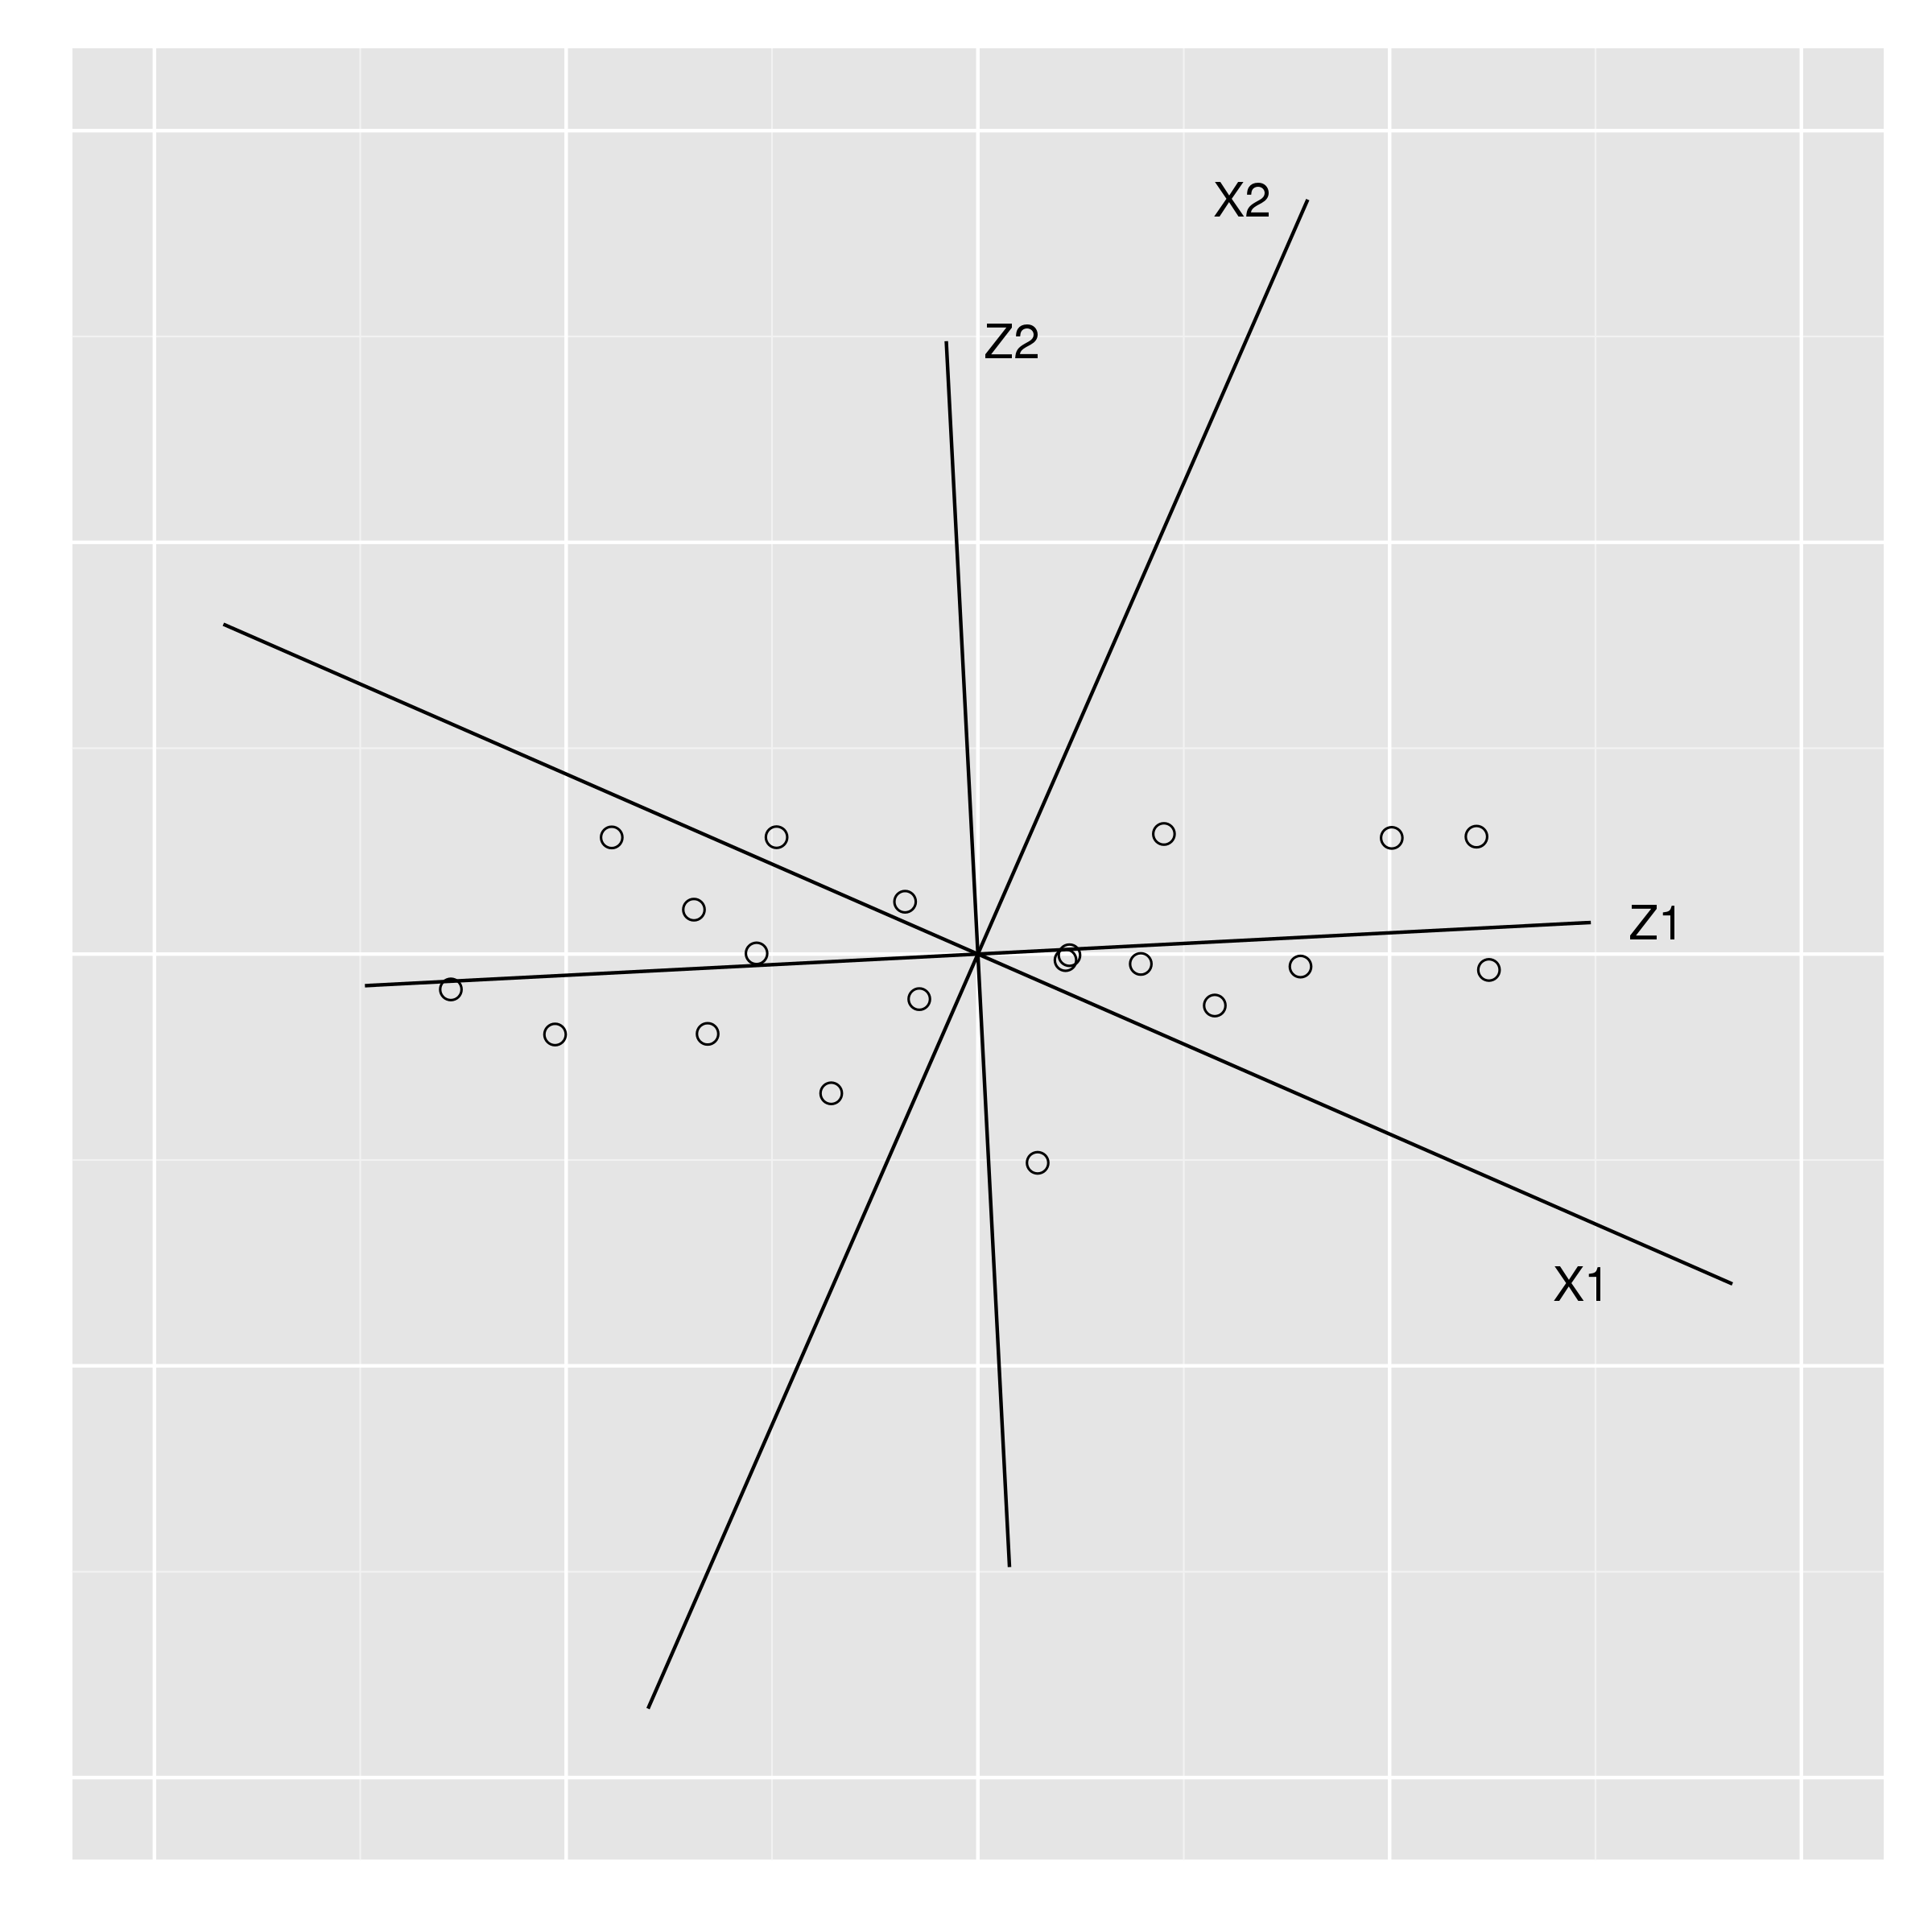
\includegraphics[height=7cm]{x1x2z1z2rotated09.png}
 \end{center}
   \end{overlayarea}
 \end{frame}
\begin{frame}\frametitle{Cambio de sistema de coordenadas}

   \begin{overlayarea}{\textwidth}{8cm} 
 \begin{center}
   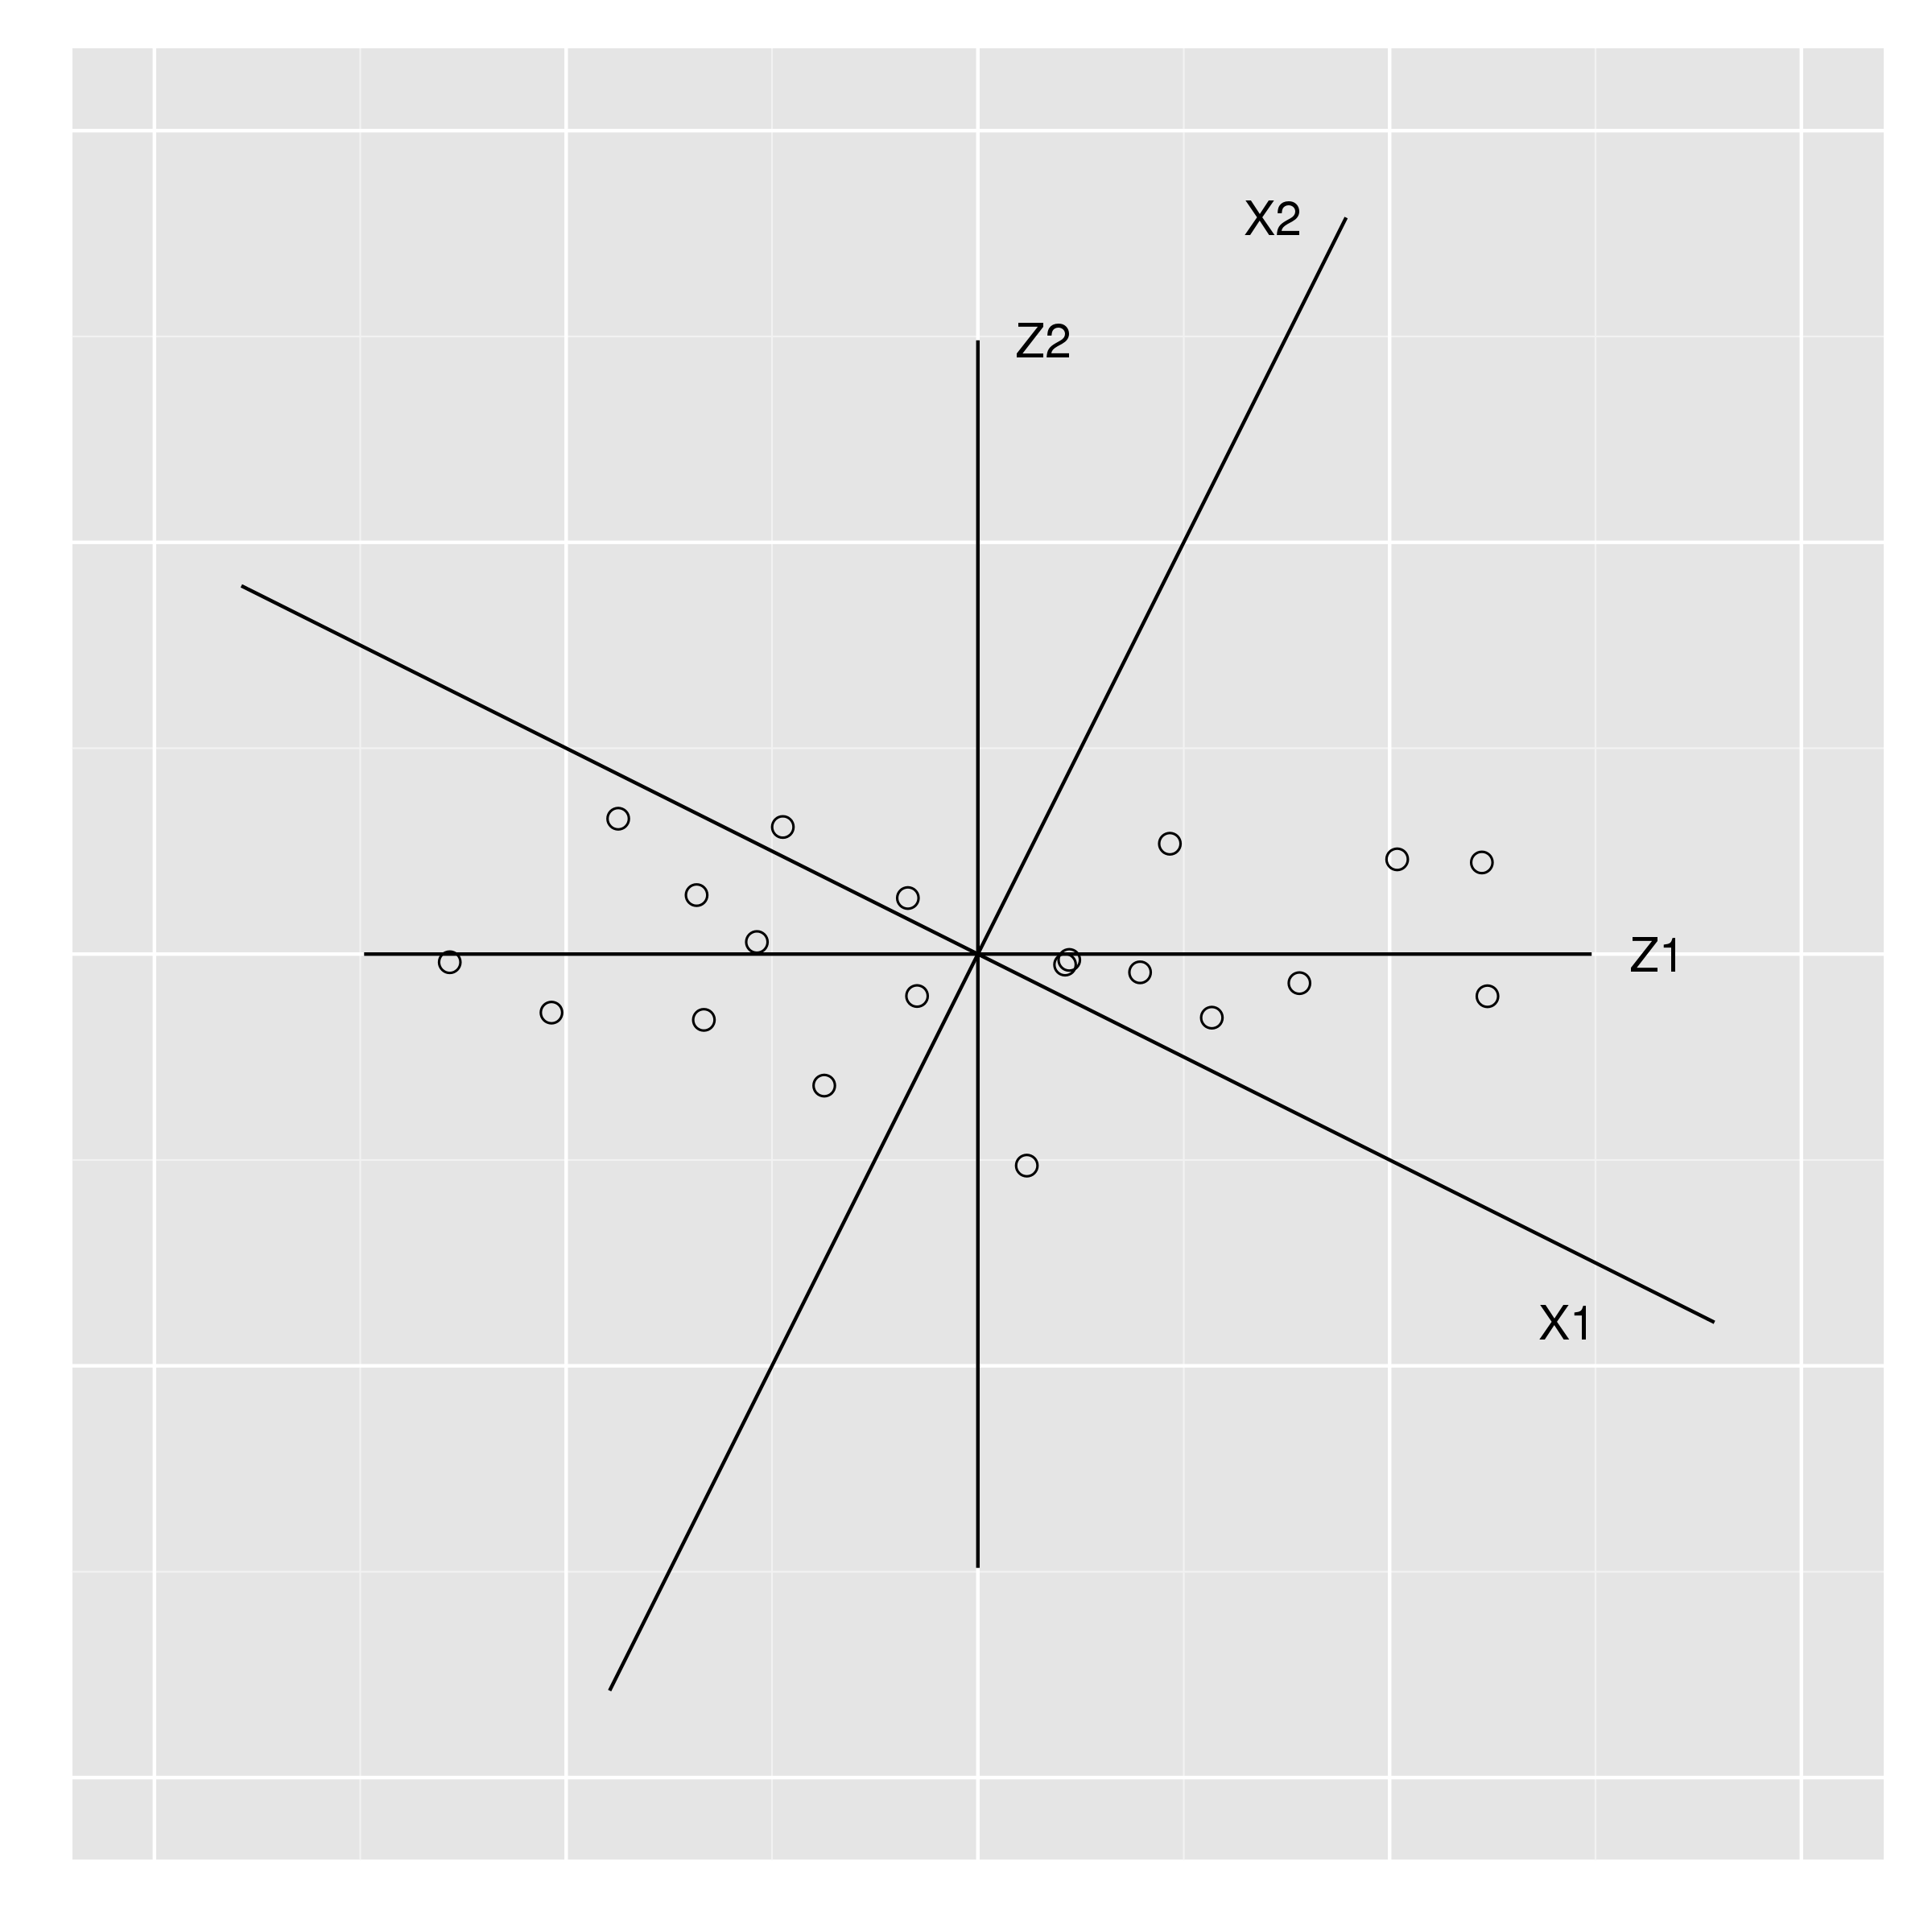
\includegraphics[height=7cm]{x1x2z1z2rotated10.png}
 \end{center}
   \end{overlayarea}
 \end{frame}
\begin{frame}\frametitle{Cambio de sistema de coordenadas}

   \begin{overlayarea}{\textwidth}{8cm} 
 \begin{center}
   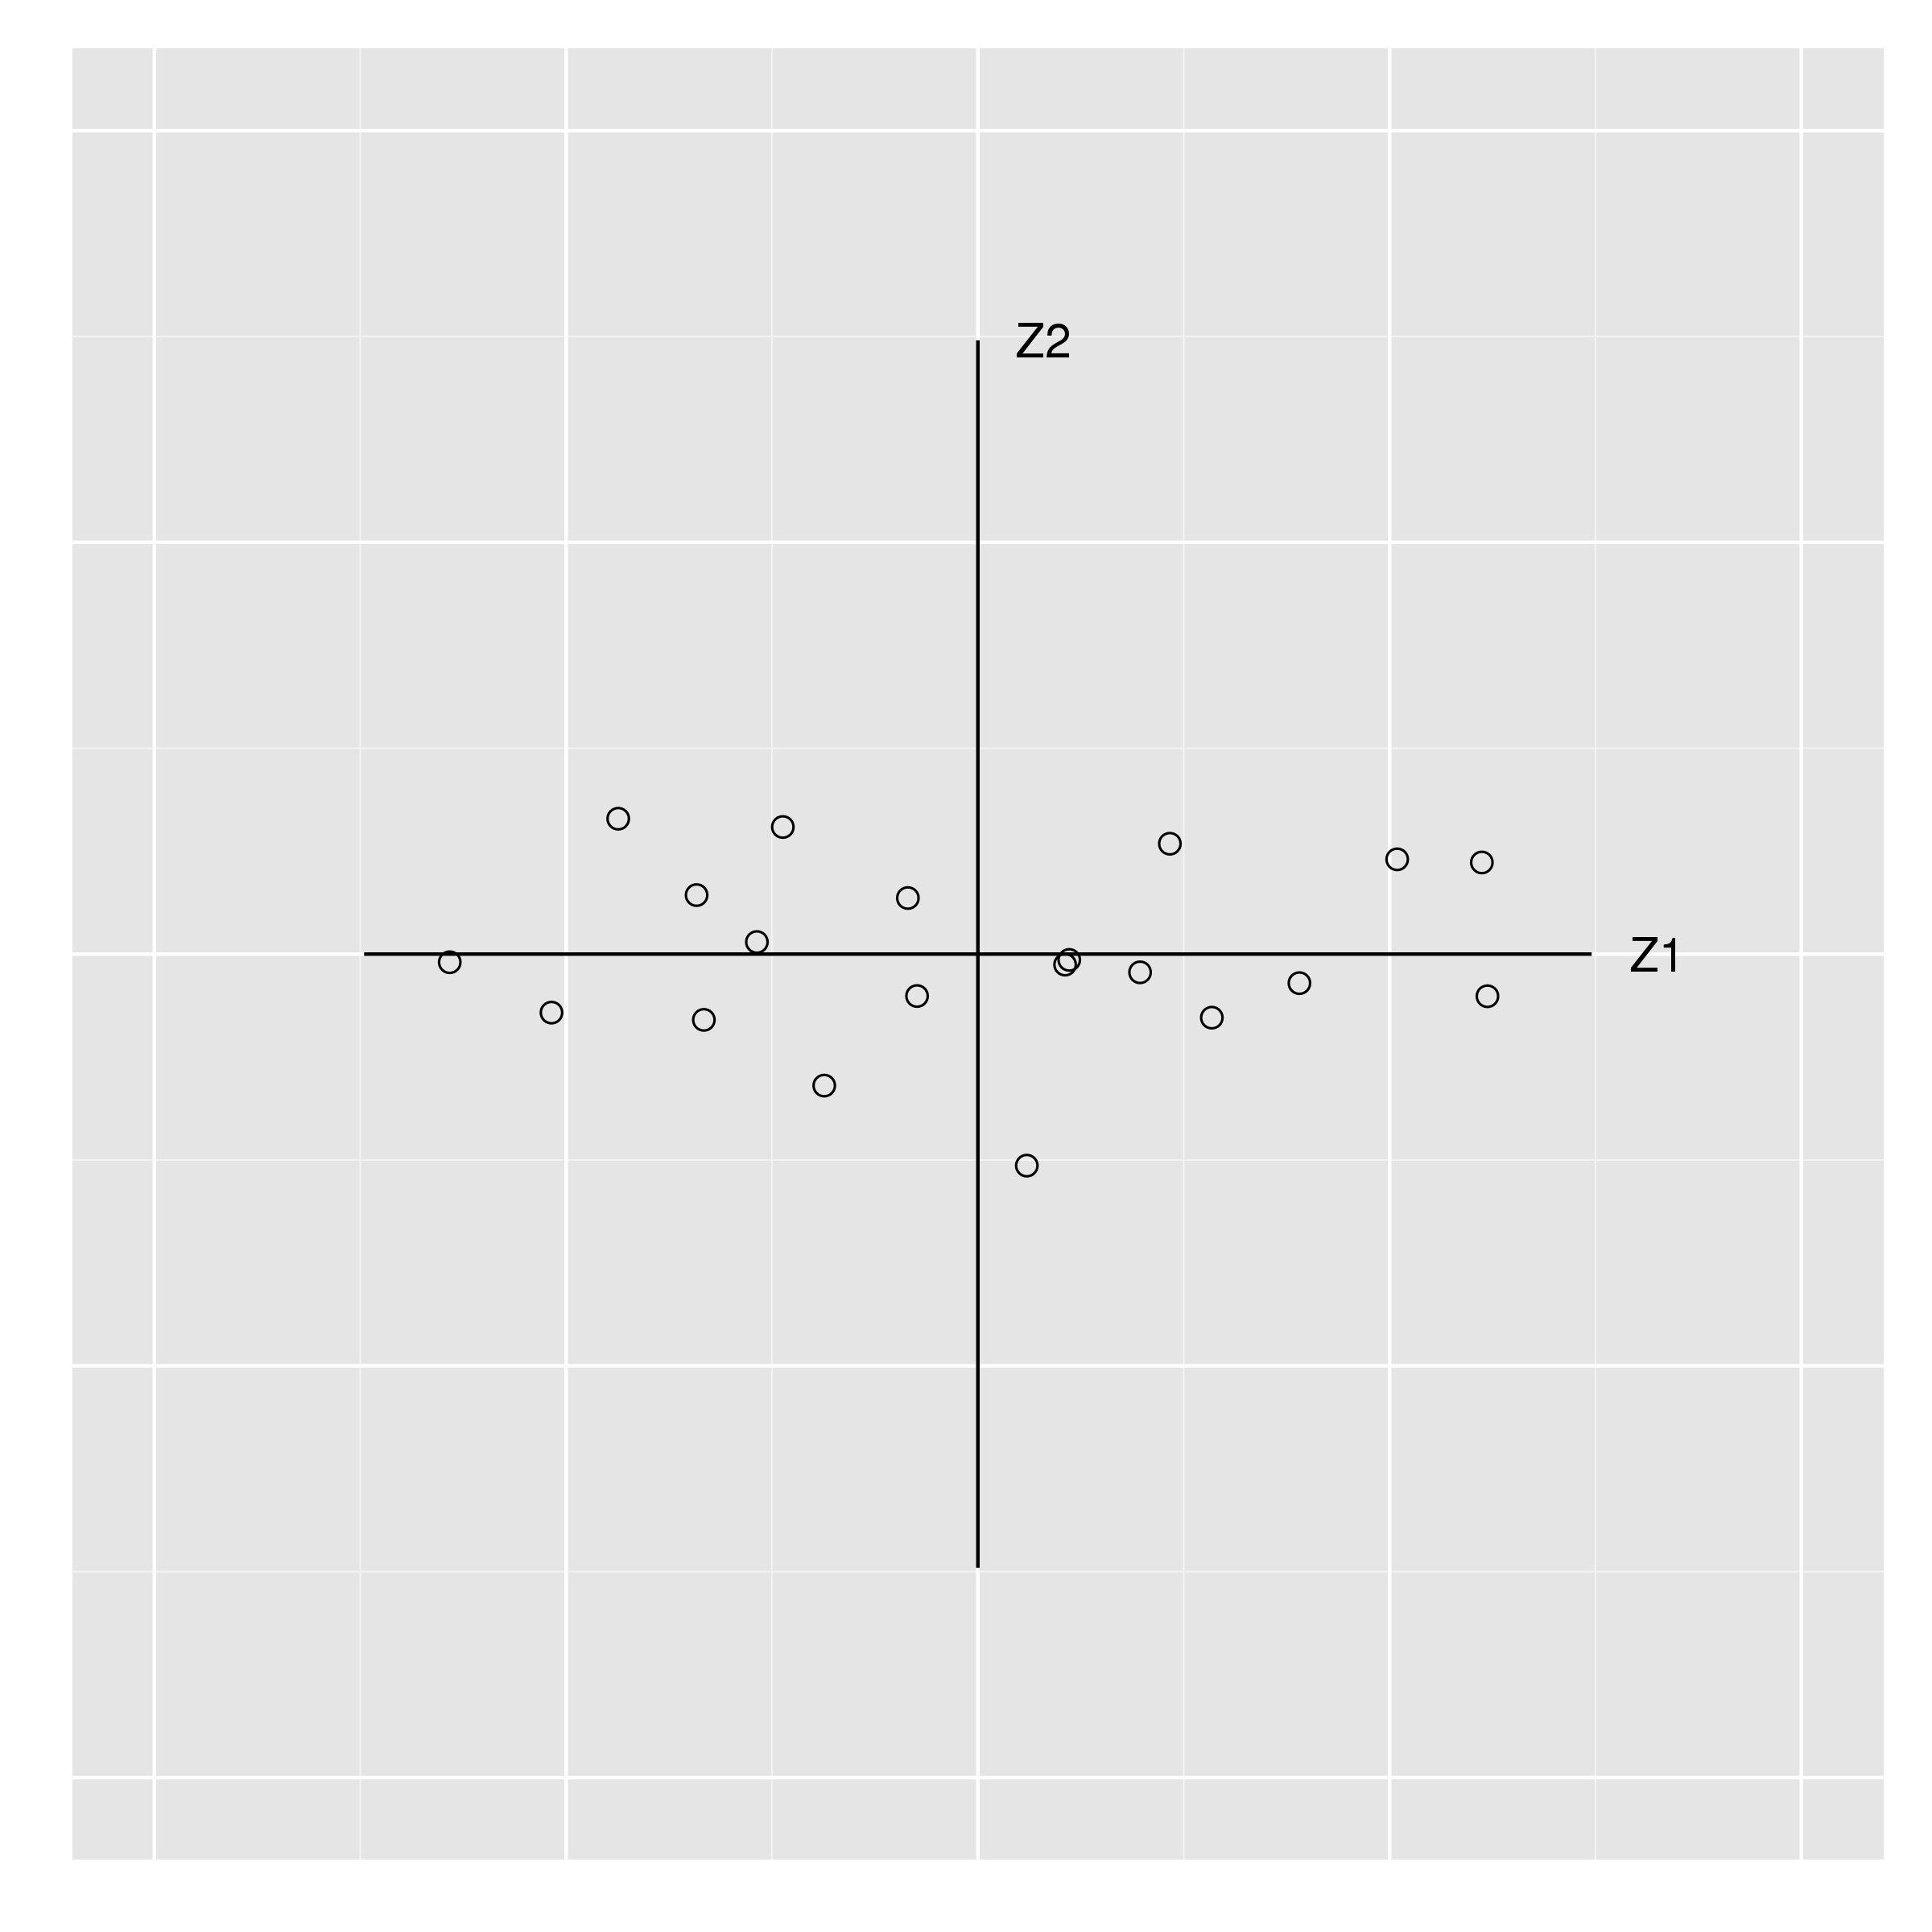
\includegraphics[height=7cm]{x1x2z1z2rotated11.png}
 \end{center}
   \end{overlayarea}
 \end{frame}

\begin{frame}\frametitle{Qué conseguimos con el cambio}
   \begin{overlayarea}{\textwidth}{8cm} 
     \begin{tabular}{p{.40\textwidth}@{\extracolsep{1mm}} m{.60\textwidth}}
\raisebox{-0.5\totalheight}{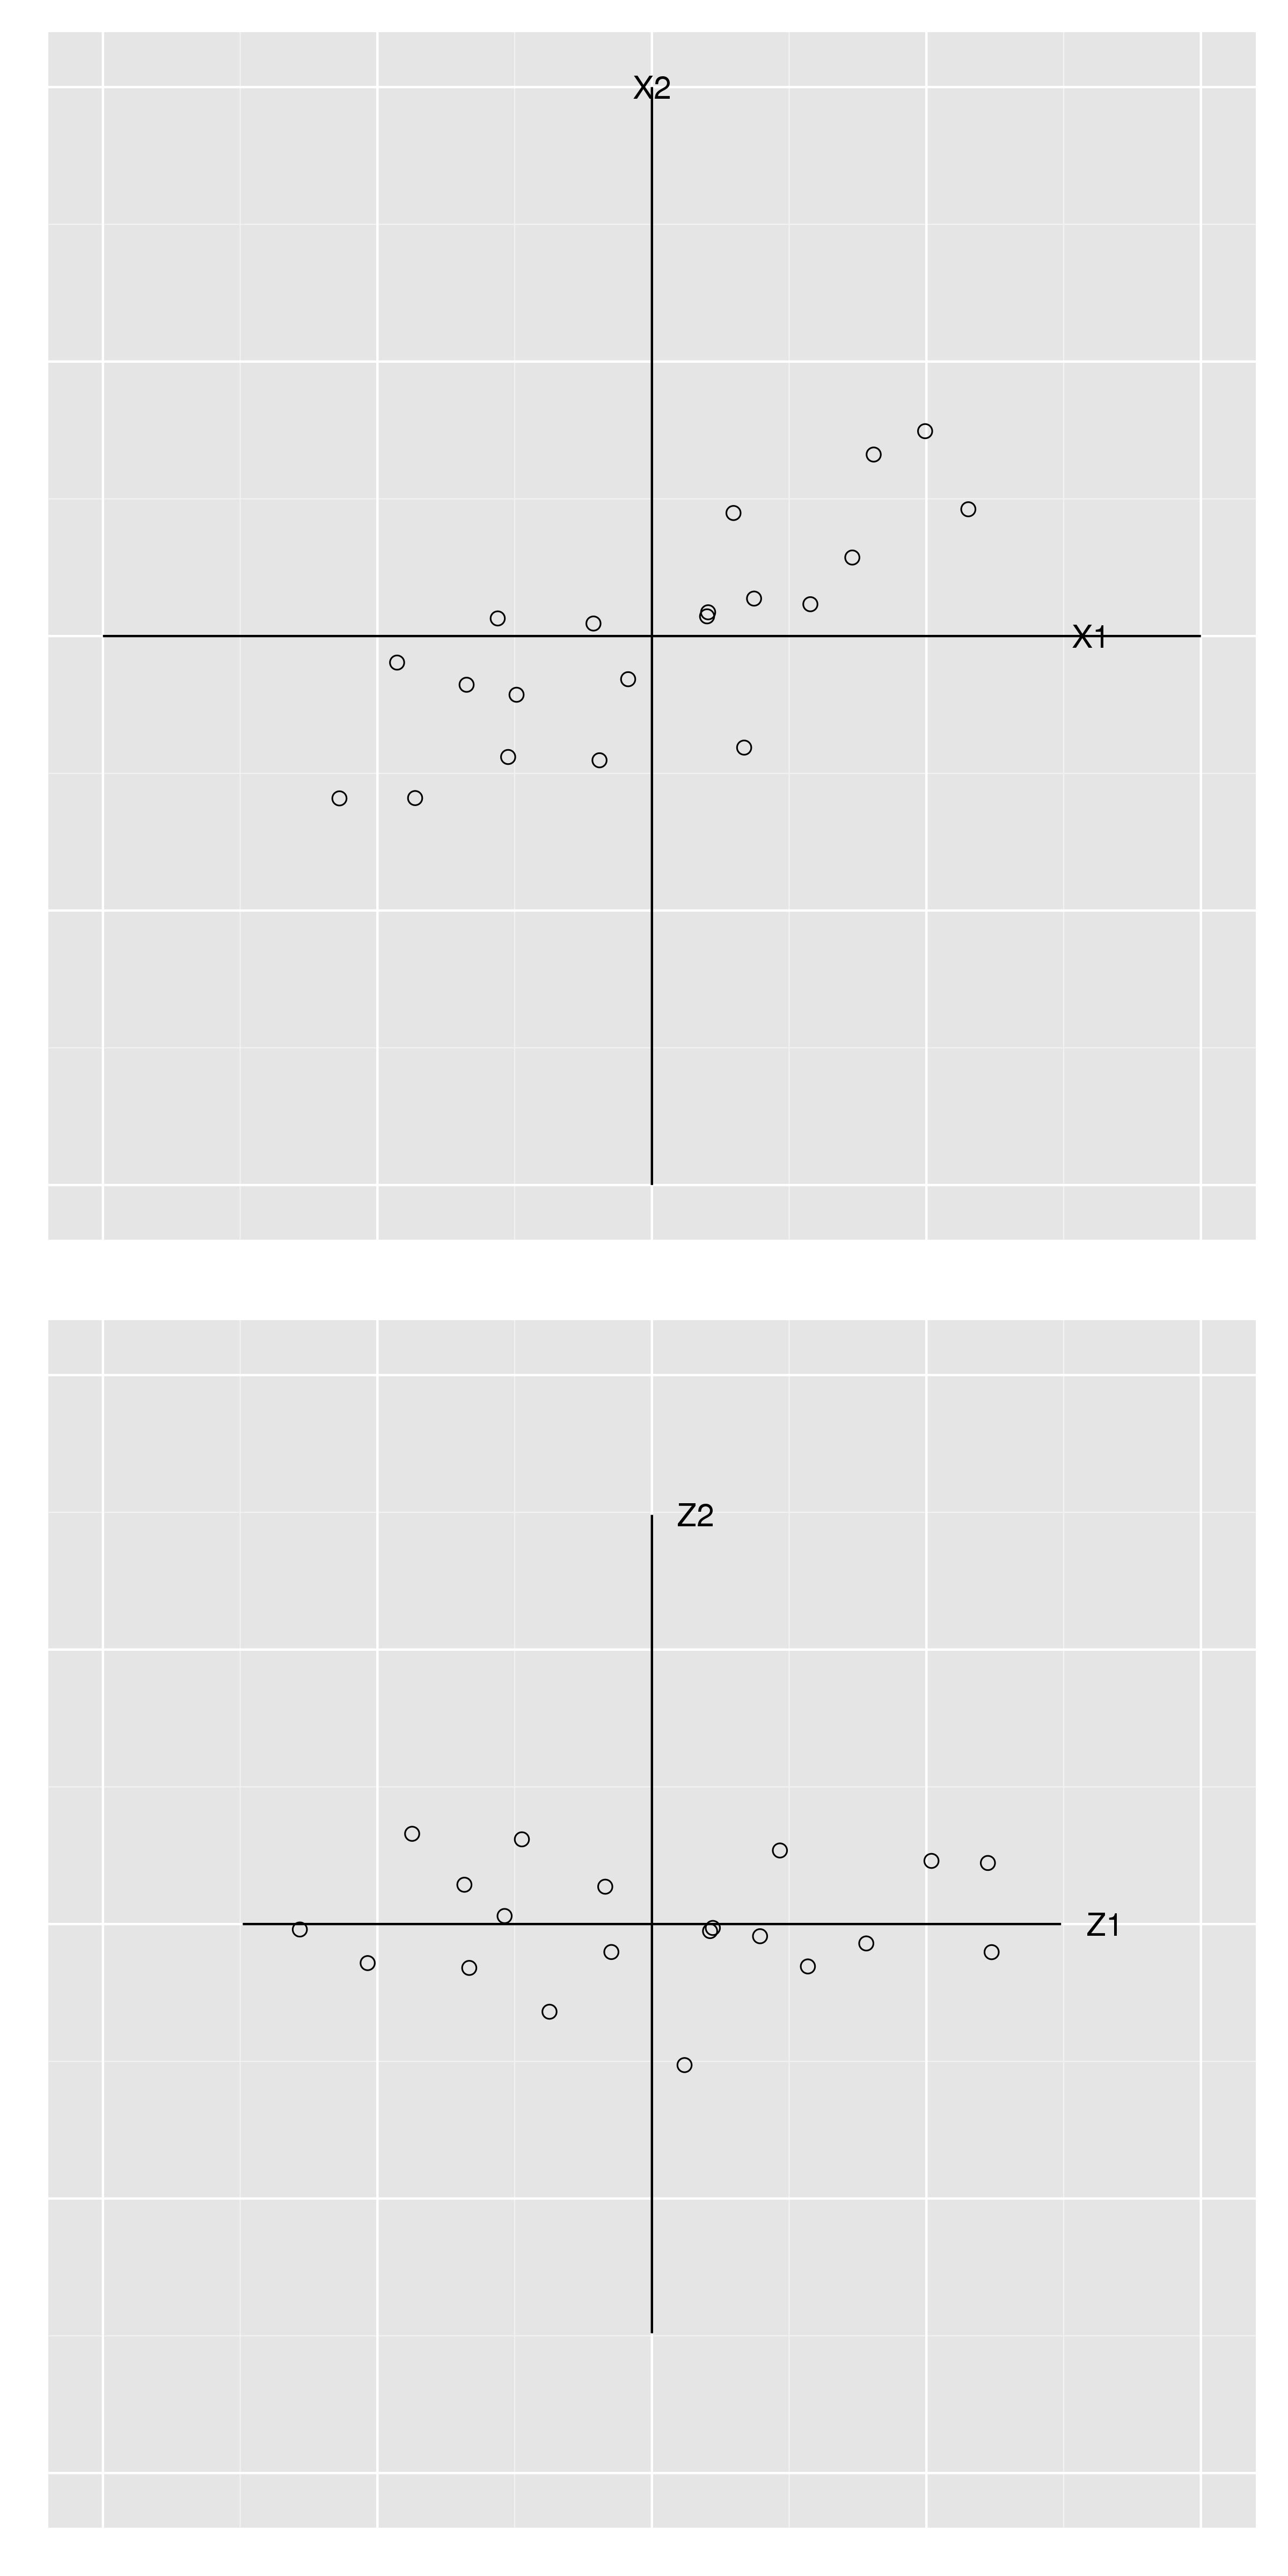
\includegraphics[width=4cm]{dosx1x2z1z2.png}} &       \begin{minipage}{6.5cm}
 \vspace{-1.5cm}\onslide<2->$\bullet$ La descripción es equivalente en los dos sistemas de coordenadas\\
  \onslide<3-> $\bullet$ Pero la variabilidad de las componentes en los dos sistemas es diferente:
    \begin{itemize}
    \item<4-> $Var(X_1)=11.2$, $Var(X_2)=3.84$.
    \item<5-> $Var(Z_1)=11.13$, $Var(Z_2)=0.93$.
  \end{itemize}
\onslide<6-> En la segunda representación, la variabilidad de  $Z_2$ es pequeña respecto a la variabilidad de $Z_1$.\\
\onslide<7-> $\Rightarrow$ si tenemos que resumir, nos podemos quedar con $Z_1$ sólo...\\
\onslide<8-> $\bullet$ $Z_1$ y $Z_2$ son incorrelados.
       \end{minipage}
     \end{tabular}
   \end{overlayarea}
 \end{frame}
 
  \begin{frame}\frametitle{Reducimos la dimensión}
  Consideramos la componente Z1:
 \begin{center}
   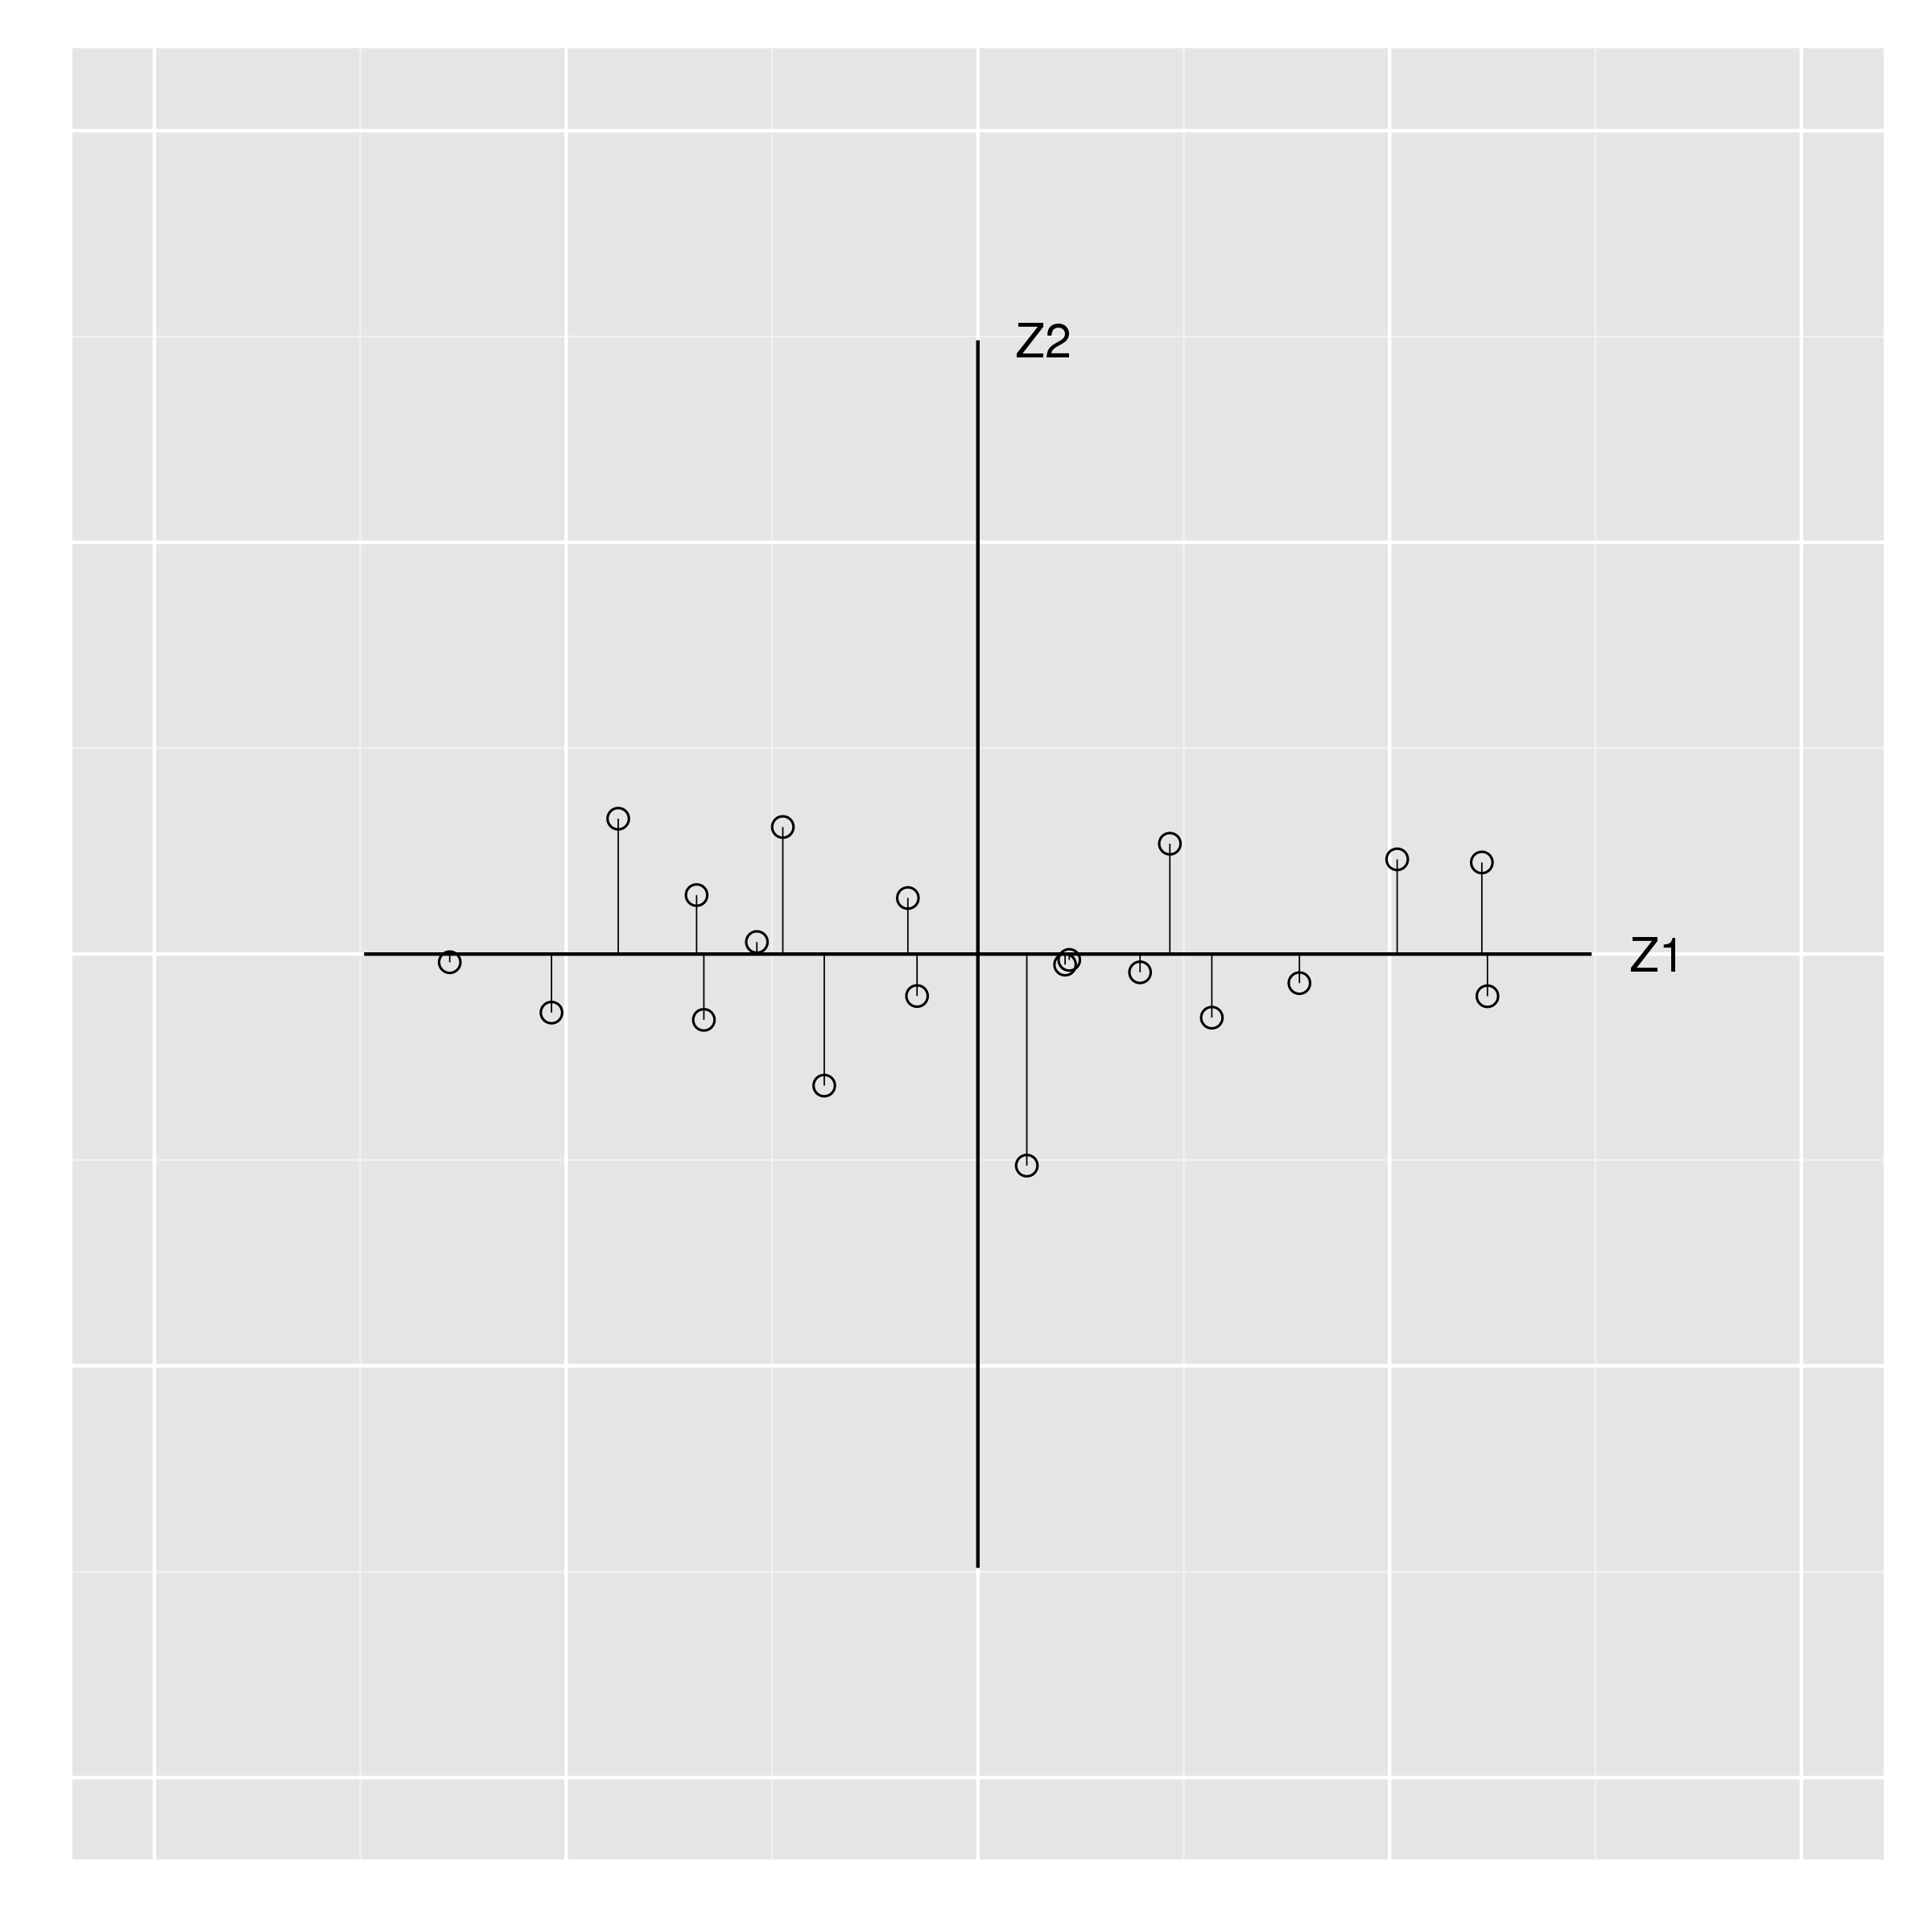
\includegraphics[height=7cm]{reduccion2d1d_1.png}
 \end{center}
  \end{frame}
  \begin{frame}\frametitle{Reducimos la dimensión}
  Consideramos la componente Z1:
 \begin{center}
   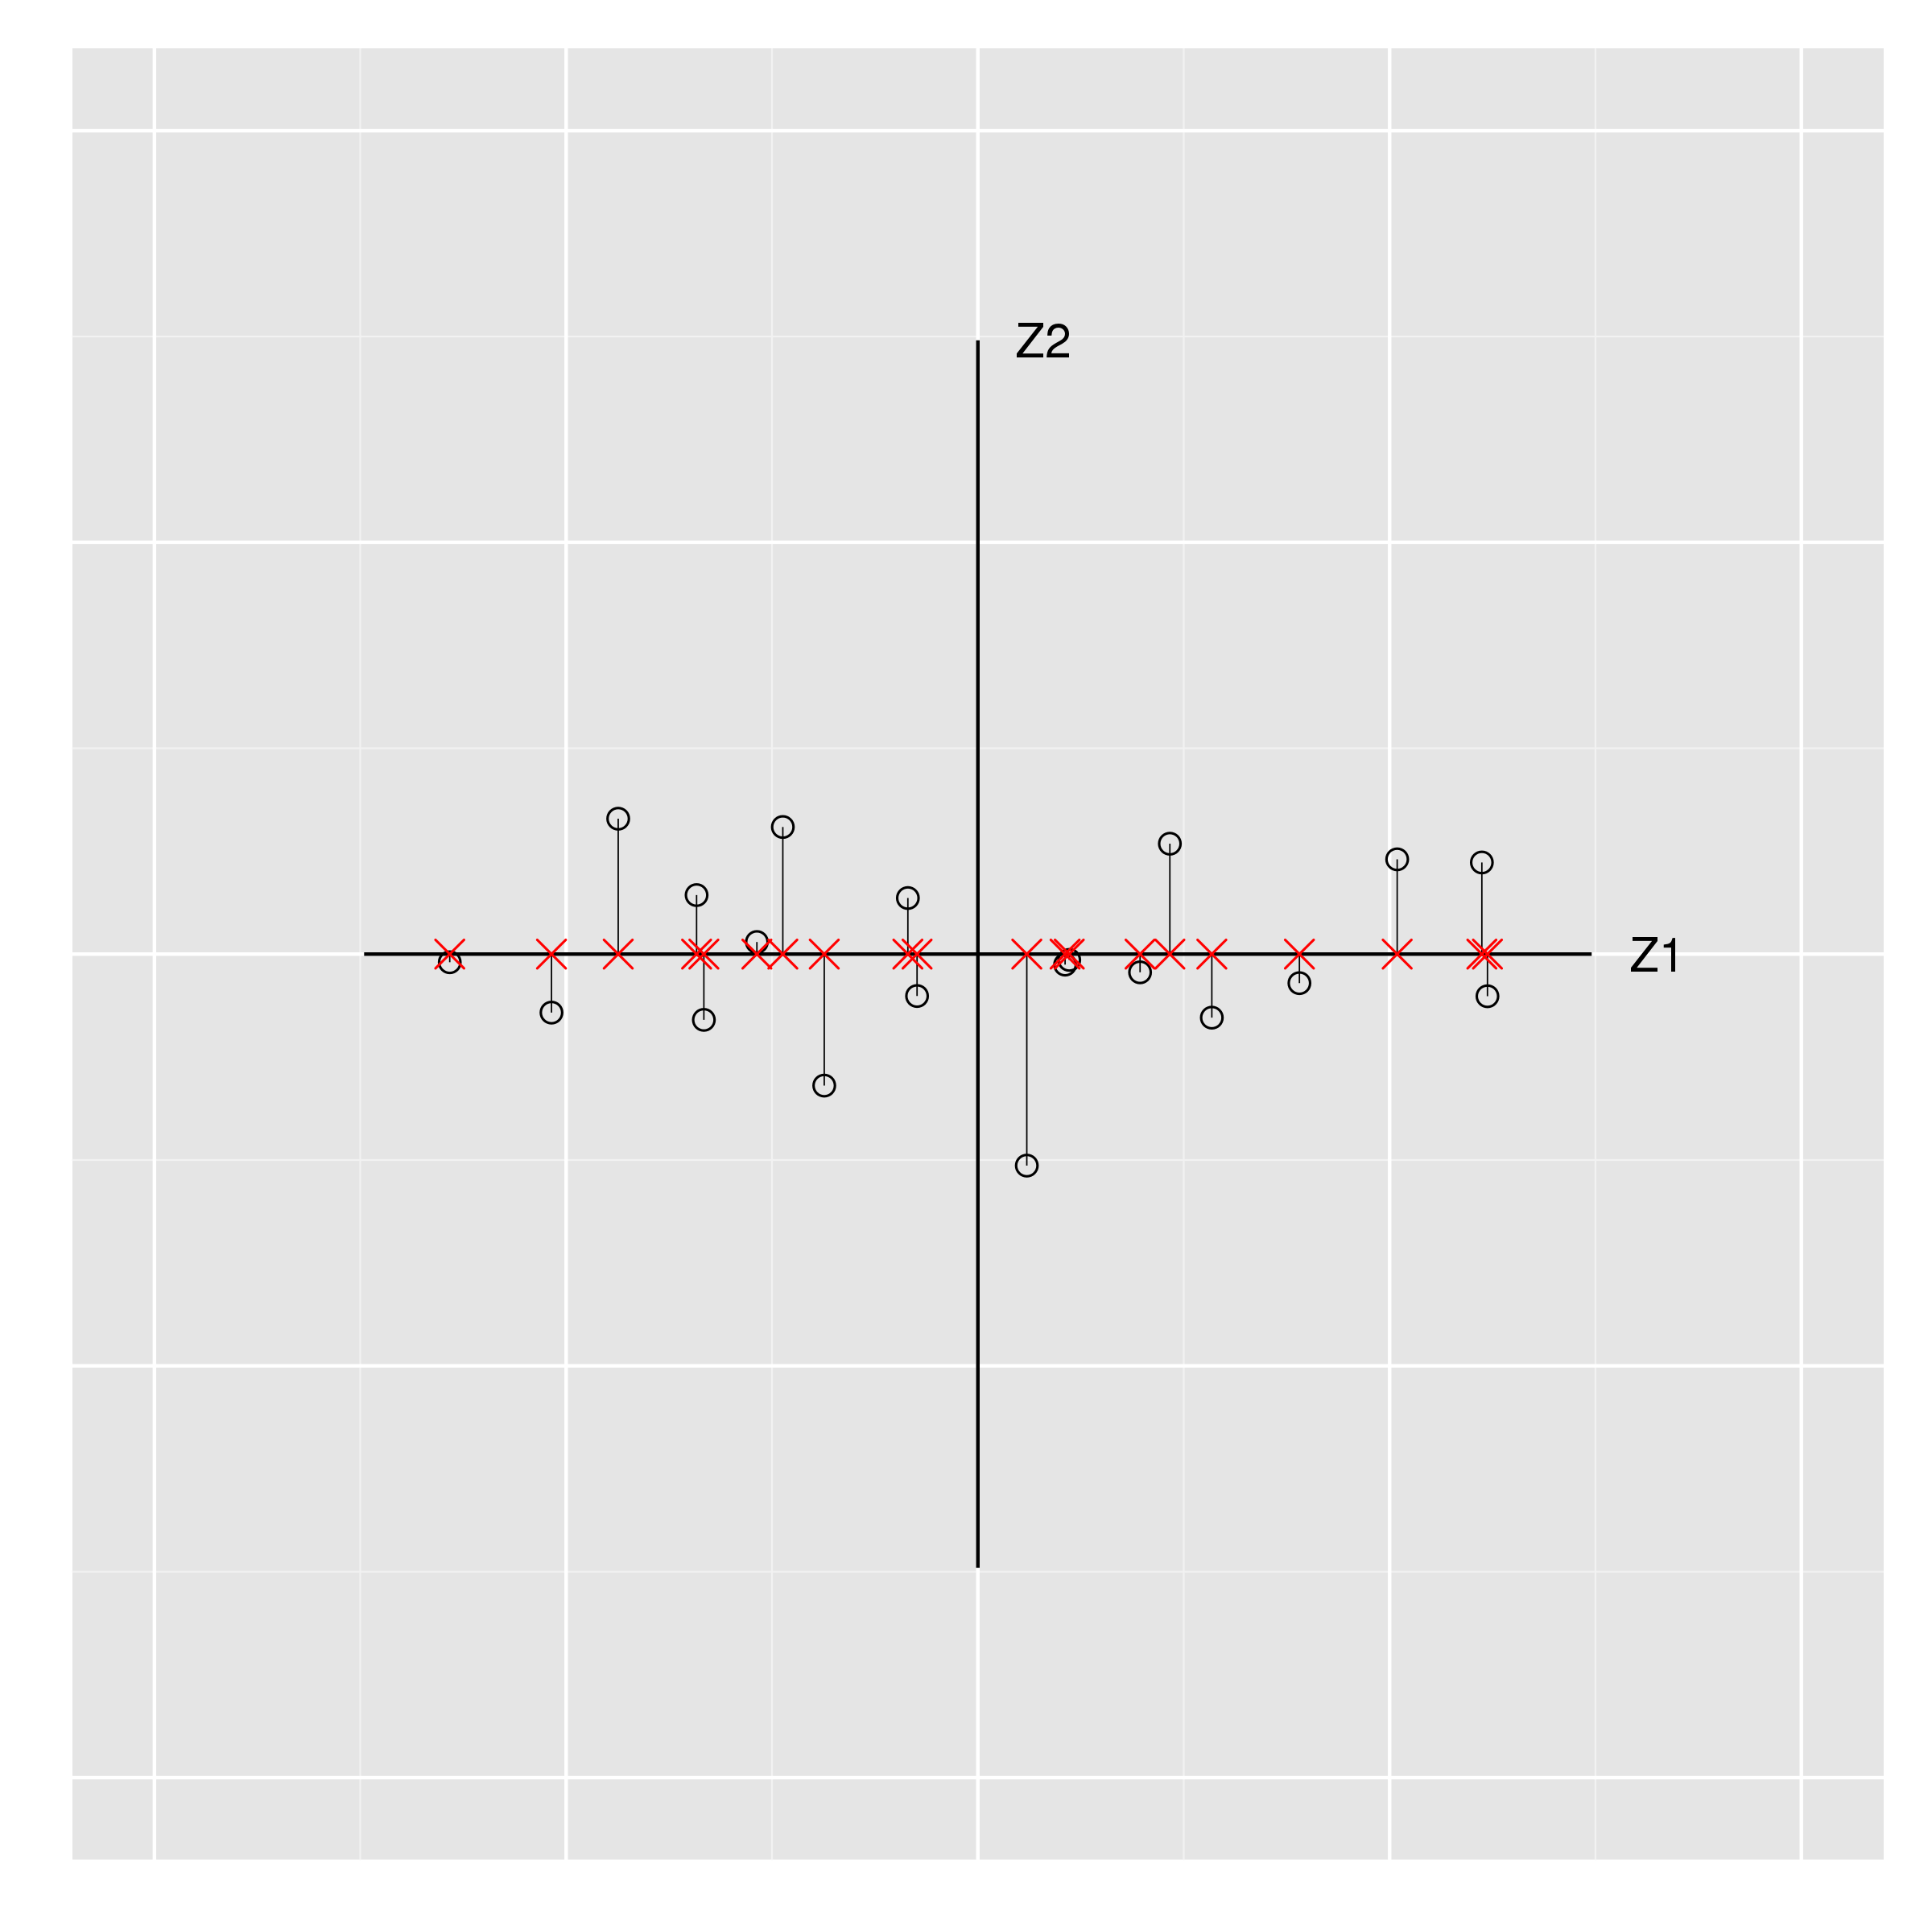
\includegraphics[height=7cm]{reduccion2d1d_2.png}
 \end{center}
  \end{frame}
  \begin{frame}\frametitle{Reducimos la dimensión}
  Consideramos la componente Z1:
 \begin{center}
   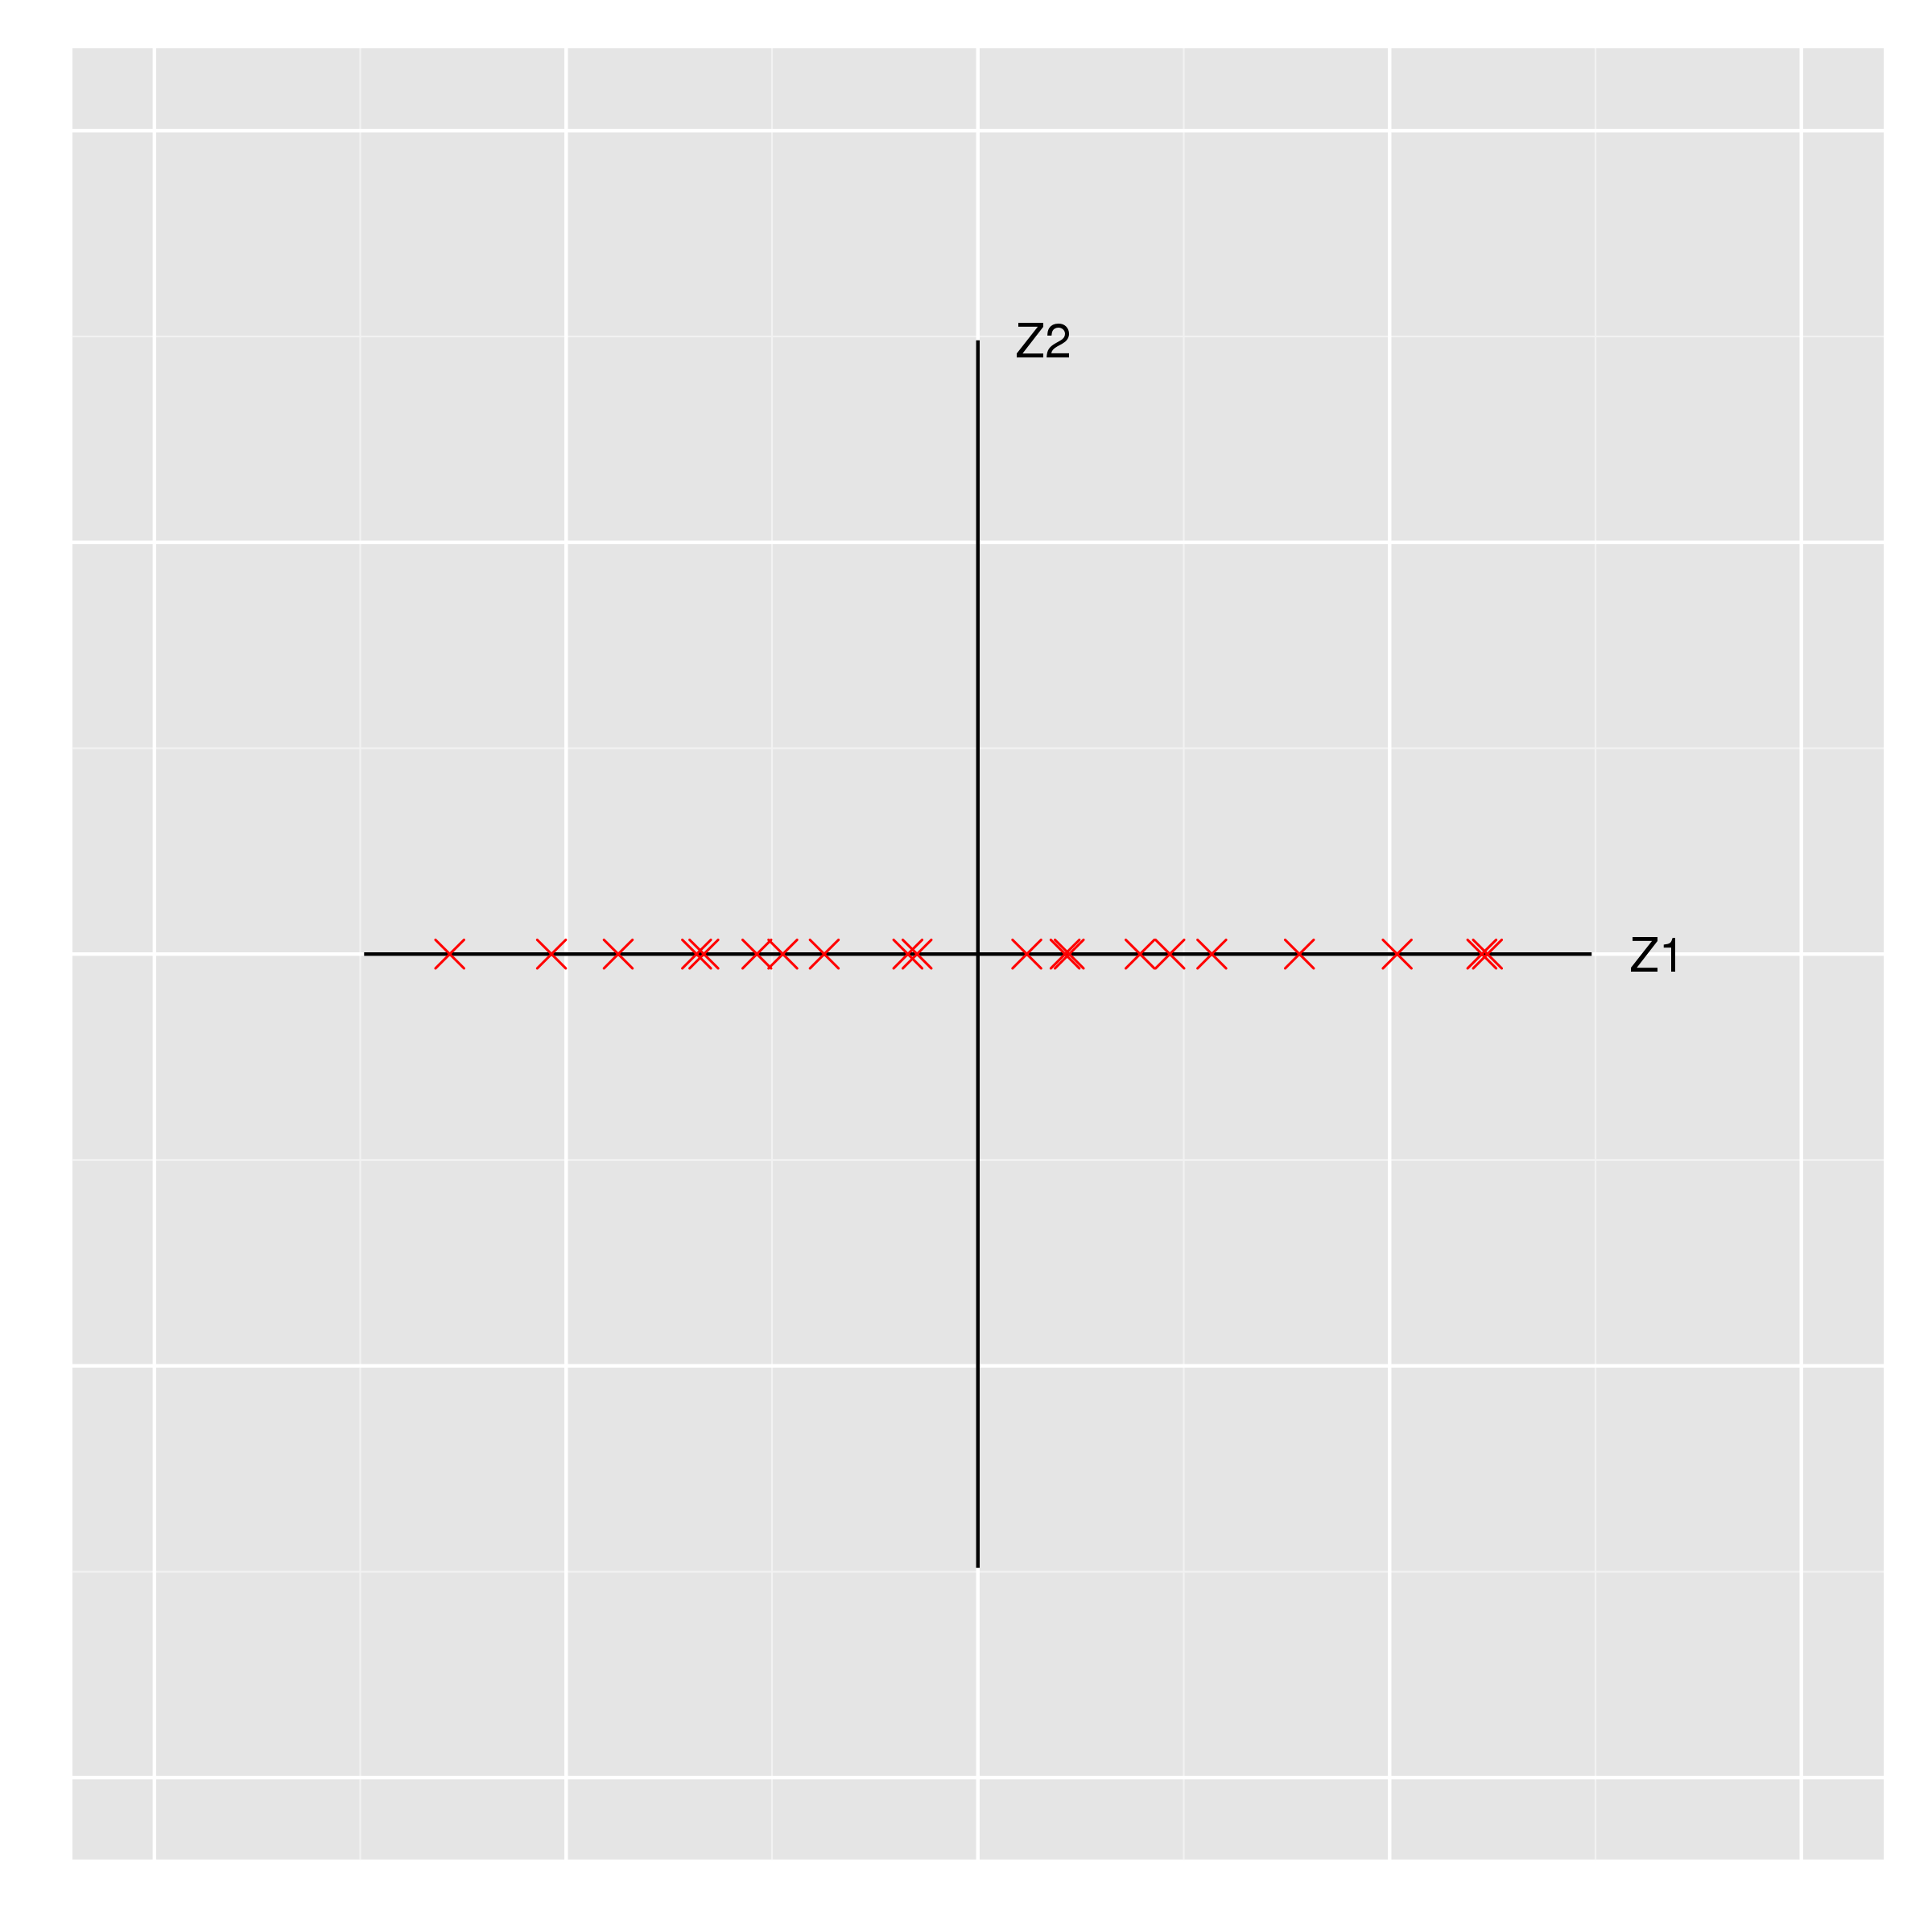
\includegraphics[height=7cm]{reduccion2d1d_3.png}
 \end{center}
  \end{frame}
  \begin{frame}\frametitle{Reducimos la dimensión}
  Consideramos la componente Z1:
 \begin{center}
   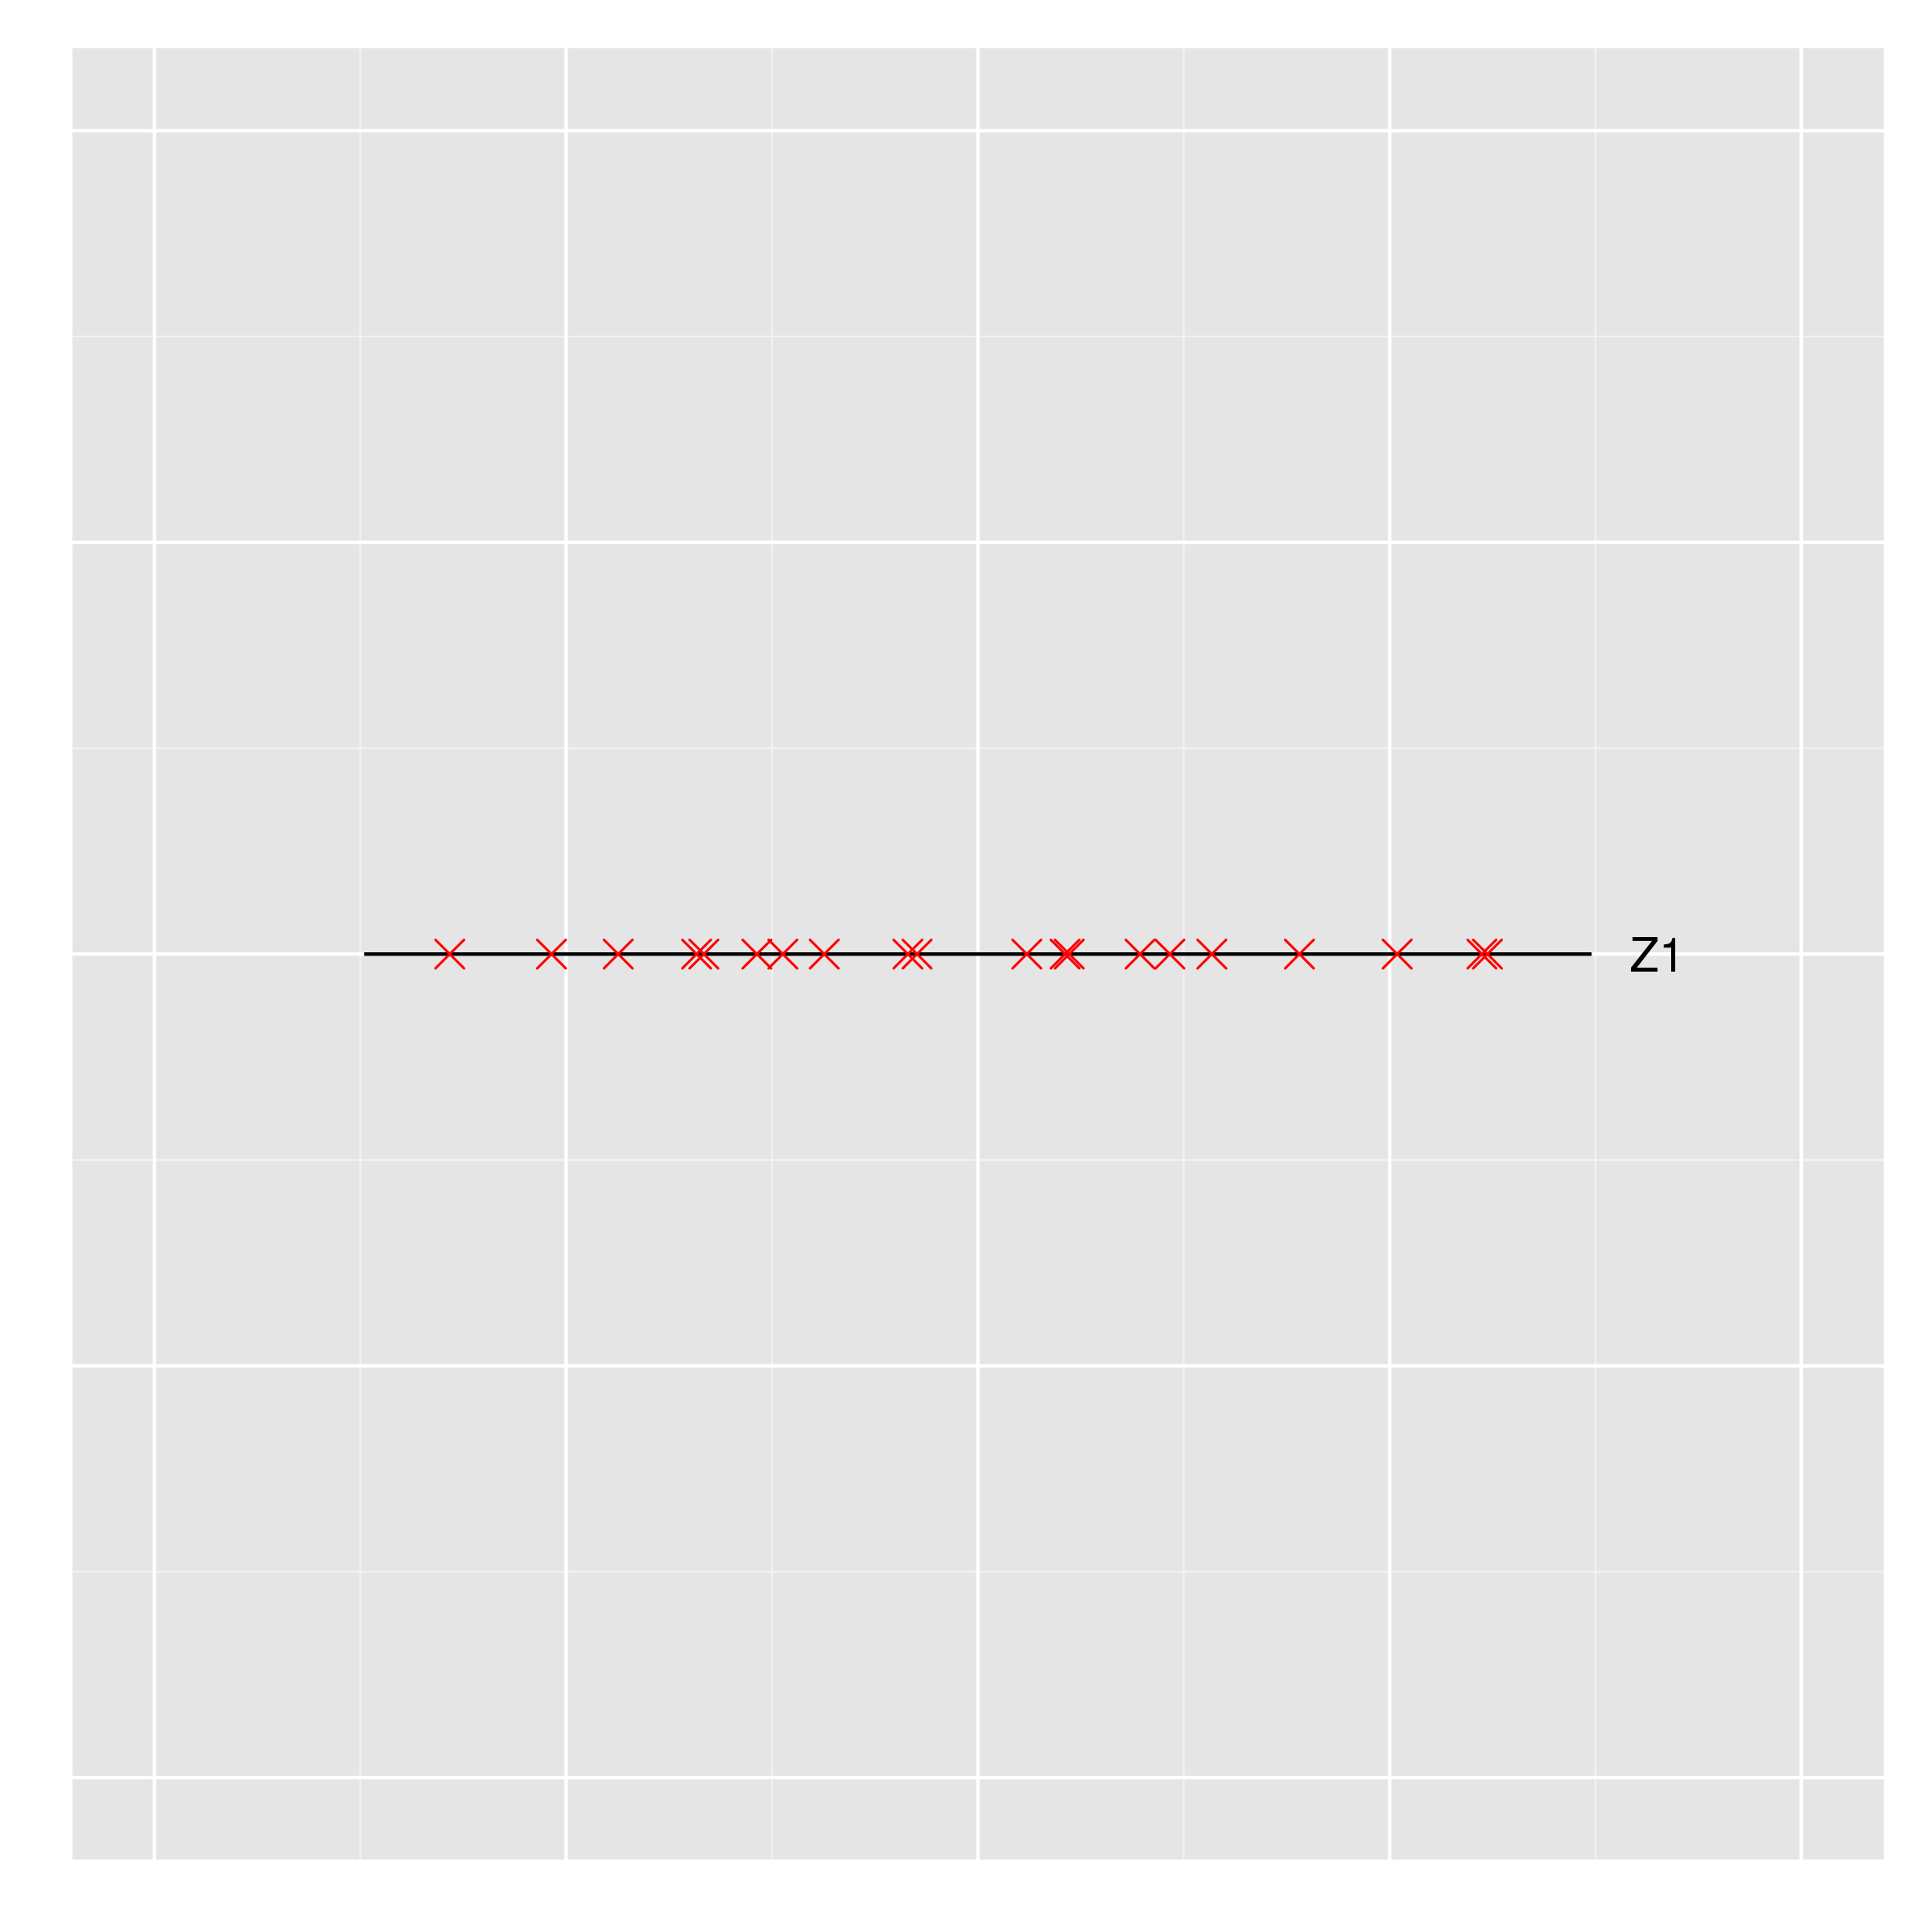
\includegraphics[height=7cm]{reduccion2d1d_4.png}
 \end{center}
  \end{frame}


 \begin{frame}\frametitle{Reducción de dimensión}
      \begin{overlayarea}{\textwidth}{6cm} 
{\tiny $$X=\left(\begin{array}{rr}
  1.360&  0.705\\
 -2.115& -0.720\\
 -2.460&  0.670\\
  \vdots & \vdots\\
  4.000&  1.775\\
 -0.080& -0.440\\
 -3.960& -2.605\\
 -2.270& -1.860\\
\end{array}\right) \xrightarrow[coordenadas]{Cambio\ de}
 Z=\left(\begin{array}{rr}
 0.947&   0.114\\
-2.400& -0.131\\
-2.118&  -1.380\\
  \vdots & \vdots\\
 3.492& 0.315\\
-0.660& 0.455\\
-4.631& 0.635\\
-2.976& 0.714\\
\end{array}\right) \xrightarrow[dim.]{Reducc.\ de}
 \hat{Z}=\left(\begin{array}{r}
 0.947   \\
-2.400   \\
-2.118   \\
  \vdots \\
 3.492   \\
-0.660   \\
-4.631   \\
-2.976   \\
\end{array}\right) 
 $$}

      \end{overlayarea}
 \end{frame}  
 \begin{frame}\frametitle{Reducción de dimensión}
Ejemplo en 3D.
 \end{frame}

  \begin{frame}\frametitle{Planteamiento general: preliminares}
    \begin{itemize}
    \item<+-> Sea $\vec{x_1},\ldots,\vec{x}_k$ una base de $\R^k$. Nube de puntos $k$-dimensional de $n$ puntos $M_1$, $M_2,\ldots,M_n$.
    \item<+-> $(x_{i1},x_{i2},\ldots,x_{ik})$ son las coordenadas del punto $M_i$ en la base $\vec{x_1},\ldots,\vec{x}_k$.
    \item<+-> Consideramos la matriz
         \begin{equation*}
X=\left(\begin{array}{llll}
x_{11}&x_{12}&\cdots&x_{1k}\\
x_{21}&x_{22}&\cdots&x_{2k}\\
\vdots&\vdots&\vdots&\vdots\\
x_{n1}&x_{n2}&\cdots&x_{nk}\\
\end{array}\right).
\end{equation*}

    \end{itemize}
    
 \end{frame}

    \begin{frame}\frametitle{Planteamiento general: preliminares}
    \begin{itemize}
    \item<+-> Escogemos otra base $\vec{u}_1,\ldots,\vec{u}_k$ de $\R^k$.
    \item<+-> Sean $(z_{i1},z_{i2},\ldots,z_{ik})$  las coordenadas del punto $M_i$ en esta nueva base
        \item<+-> Consideramos la matriz
          $$Z=\left(\begin{array}{llll}
z_{11}&z_{12}&\cdots&z_{1k}\\
z_{21}&z_{22}&\cdots&z_{2k}\\
\vdots&\vdots&\vdots&\vdots\\
z_{n1}&z_{n2}&\cdots&z_{nk}\\
\end{array}\right),$$
de las coordenadas de los puntos de la nube.
    \end{itemize}
    
 \end{frame}
      \begin{frame}\frametitle{Planteamiento general: preliminares}
    \begin{itemize}
    \item<+-> Para relacionar $Z$ con $X$, escribimos la matriz de paso de la base base $\vec{x}_1,\ldots,\vec{x}_k$ a la nueva base.
    \item<+-> La matriz $U$, es la matriz $k\times k$ cuyas columnas contienen las coordenadas de los vectores $\vec{u}_1,\ldots,\vec{u}_k$ en la base inicial, es decir si
\begin{eqnarray*}
\vec{u}_1&=&u_{11}\vec{x}_1+u_{21}\vec{x}_2+\cdots+u_{k1}\vec{x}_k\\
\vec{u}_2&=&u_{12}\vec{x}_1+u_{22}\vec{x}_2+\cdots+u_{k2}\vec{x}_k\\
\vdots&\vdots\\
\vec{u}_k&=&u_{1k}\vec{x}_1+u_{2k}\vec{x}_2+\cdots+u_{kk}\vec{x}_k,\\
\end{eqnarray*}    \end{itemize}
    
 \end{frame}
      \begin{frame}\frametitle{Planteamiento general: preliminares}
    \begin{itemize}
    \item ....   si
\begin{eqnarray*}
\vec{u}_1&=&u_{11}\vec{x}_1+u_{21}\vec{x}_2+\cdots+u_{k1}\vec{x}_k\\
\vec{u}_2&=&u_{12}\vec{x}_1+u_{22}\vec{x}_2+\cdots+u_{k2}\vec{x}_k\\
\vdots&\vdots\\
\vec{u}_k&=&u_{1k}\vec{x}_1+u_{2k}\vec{x}_2+\cdots+u_{kk}\vec{x}_k,
\end{eqnarray*}
la matriz de paso será\vspace{-0.2cm} 
$$\label{paso}U=\left(\begin{array}{llll}
u_{11}&u_{12}&\cdots&u_{1k}\\
u_{21}&u_{22}&\cdots&u_{2k}\\
\vdots&\vdots&\vdots&\vdots\\
u_{k1}&u_{k2}&\cdots&u_{kk}\\
\end{array}\right).$$
    \end{itemize}
    
 \end{frame}
        \begin{frame}\frametitle{Planteamiento general: preliminares}
    \begin{itemize}
    \item<+-> La relación entre  $Z$, $X$ y $U$ es 
\begin{equation*}
X=ZU^T,
\end{equation*}
\item<+-> $U$ es invertible , por lo que 
\begin{equation*}
X(U^T)^{-1}=Z.
\end{equation*}
\item<+->  Si los vectores $\vec{u}_1,\ldots,\vec{u}_k$ forman una base ortonormal, la matriz $U$ satisface $U^TU=Id$, y por lo tanto $(U^T)^{-1}=U$: $$Z=XU.$$
    \end{itemize}
    
 \end{frame}
  \begin{frame}\frametitle{      Matriz de covarianzas y cambio de bases}
    \begin{itemize}

    \item<+-> Consideremos el conjunto de datos representado por la matriz $X$. La matriz de covarianzas de las variables $X_1,\ldots,X_k$ es 
\begin{equation*}
S_X=\left(\begin{array}{llll}
s^2_{X_1}&s_{X_1X_2}&\cdots&s_{X_1X_k}\\
s_{X_1X_2}&s^2_{X_2}&\cdots&s_{X_2X_k}\\
\vdots&\vdots&\vdots&\vdots\\
s_{X_1X_k}&s_{X_2X_k}&\cdots&s^2_{X_k}\\
\end{array}\right),
\end{equation*}
donde $s^2_{X_i}$ representa la varianza de la variable $X_i$ en el conjunto y $s_{X_iX_j}$ es la covarianza de $X_i$ y $X_j$.
\item<+-> Si $X_1,\ldots,X_k$ tienen cada una media 0: 
\begin{equation*}
S_X=\frac 1 {n-1} X^TX.
\end{equation*}
    \end{itemize}
    
 \end{frame}

   \begin{frame}\frametitle{Planteamiento general: preliminares}
    \begin{itemize}
    \item<+-> Deducimos, usando la relación entre $Z$ y $X$ que 
$$S_Z=\frac 1{n-1} Z^TZ=\frac 1{n-1}U^{-1}X^TX(U^T)^{-1}=U^{-1}S_X(U^T)^{-1}.
$$
\item<+-> En el caso en que $U$ es ortogonal, 
\begin{equation*}
S_Z=U^{-1}S_XU.
\end{equation*}

    \end{itemize}
    
 \end{frame}

       \begin{frame}\frametitle{Planteamiento general: análisis en componentes principales}
    \begin{itemize}
    \item<+-> Buscamos el cambio de sistemas de coordenadas que nos permita posiblemente una reducción de dimensión.
    \item<+-> En ese nuevo sistema, queremos que haya diferencias entre las variabilidad de los componentes: la primera coordenada debe presentar la mayor varianza, la segunda, la segunda mayor varianza, etc...
\item<+-> Teniendo en cuenta
\begin{equation*}
S_Z=U^{-1}S_XU,
\end{equation*}
se conseguirá el sistema deseado si $S_Z$ es una matriz diagonal...
\item<+-> \textcolor{red}{Realizar el análisis en componentes principales, consiste en diagonalizar la matriz $S_X$...}
    \end{itemize}
    
 \end{frame}
      \begin{frame}\frametitle{Análisis en componentes principales}
              \begin{overlayarea}{\textwidth}{6.5cm} 
        \begin{itemize}
        \item<+-> Al calcular los vectores propios de la matriz $S_X$, obtenemos los coeficientes $u_{ij}$ de la matriz $U$ de paso y 
\begin{eqnarray*}
Z_1&=&u_{11}X_1+u_{21}X_2+\cdots+u_{k1}X_k\\
Z_2&=&u_{12}X_1+u_{22}X_2+\cdots+u_{k2}X_k\\
\vdots&\vdots\\
Z_k&=&u_{1k}X_1+u_{2k}X_2+\cdots+u_{kk}X_k.\\
\end{eqnarray*}\vspace{-1.5cm}
        \end{itemize}
        \only<2>{\scriptsize 1º vector propio: $\vec{u}_1=\left(\begin{array}{l} u_{11}\\ u_{21}\\\vdots \\u_{k1} \end{array}\right),\ldots,$ kº vector propio: $\vec{u}_k=\left(\begin{array}{l} u_{1k}\\ u_{2k}\\\vdots \\u_{kk} \end{array}\right).$ }
           
        \only<3->{
        \begin{block}{Componentes principales}
          
Los componentes principales $Z_1,\ldots,Z_k$ se obtienen por lo tanto como combinaciones lineales de las variables originales $X_1,\ldots,X_k$, cuyos coeficientes se deducen de la expresión de los vectores propios.

        \end{block}}
              \end{overlayarea}
 \end{frame}
      \begin{frame}\frametitle{Análisis en componentes principales: ejemplo}
    \begin{itemize}
    \item<+-> Para el ejemplo 2D que vimos al principio de la clase, tenemos 
      $$S_X=\left(\begin{array}{ll}
                    11.238& 5.194\\
                    5.194& 3.835
                  \end{array}\right),$$
    \item<+-> Usamos Python para encontrar los valores propios y vectores propios:
      {\scriptsize\begin{itemize}
      \item<+->       $\lambda_1\simeq 13.93$ y $\lambda_2\simeq 1.16$.
      \item<+-> $\vec{u}_1=\left(\begin{array}{r}0.89\\0.46
    \end{array}
      \right)$ y $\vec{u}_2=\left(\begin{array}{r} -0.46\\0.89\end{array}\right)$
      \end{itemize} }
    \item<+-> Los dos componentes principales son 
\begin{eqnarray*}
Z_1&=&0.89X_1+0.46X_2\\
Z_2&=&-0.46X_1+0.89X_2\\
\end{eqnarray*}
    \end{itemize}
 \end{frame}

  \begin{frame}\frametitle{Cambio de sistema en el ejemplo:}
  La nueva base:
 \begin{center}
   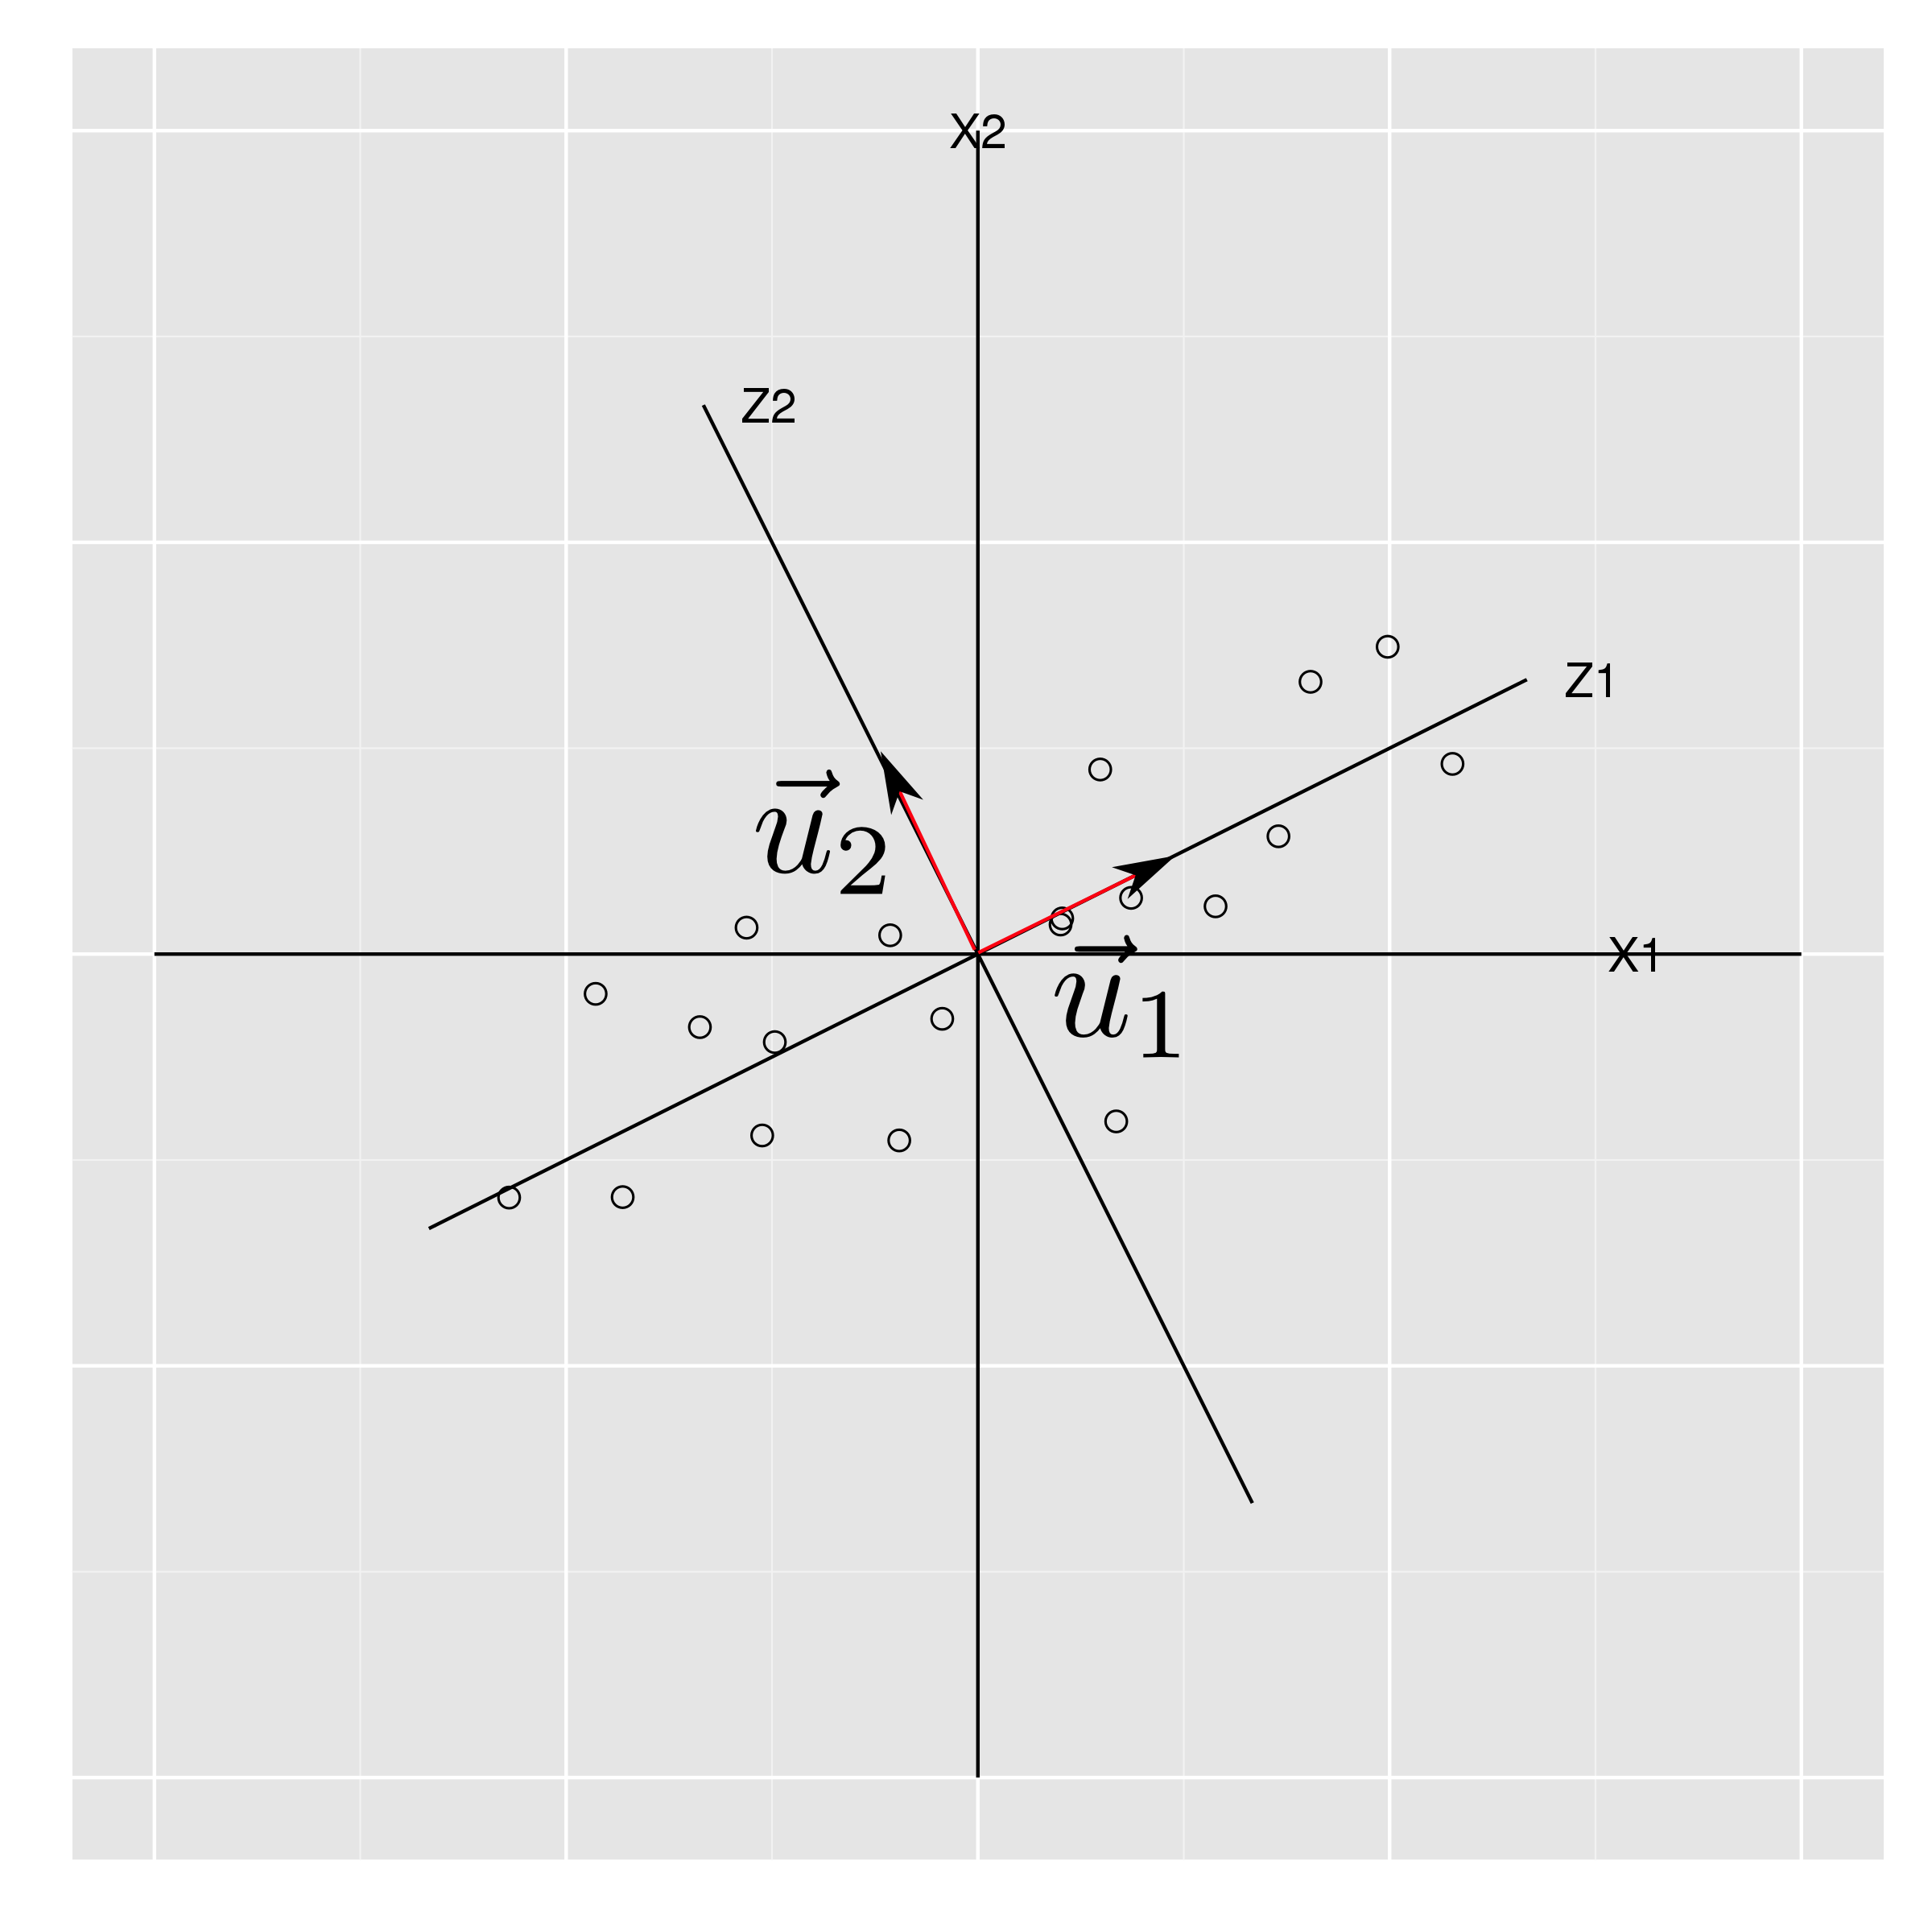
\includegraphics[height=7cm]{x1x2z1z2rotated01-convectores.png}
 \end{center}
  \end{frame}


  \begin{frame}\frametitle{Reducimos la dimensión}
  Cómo calculamos la componente Z1:
 \begin{center}
   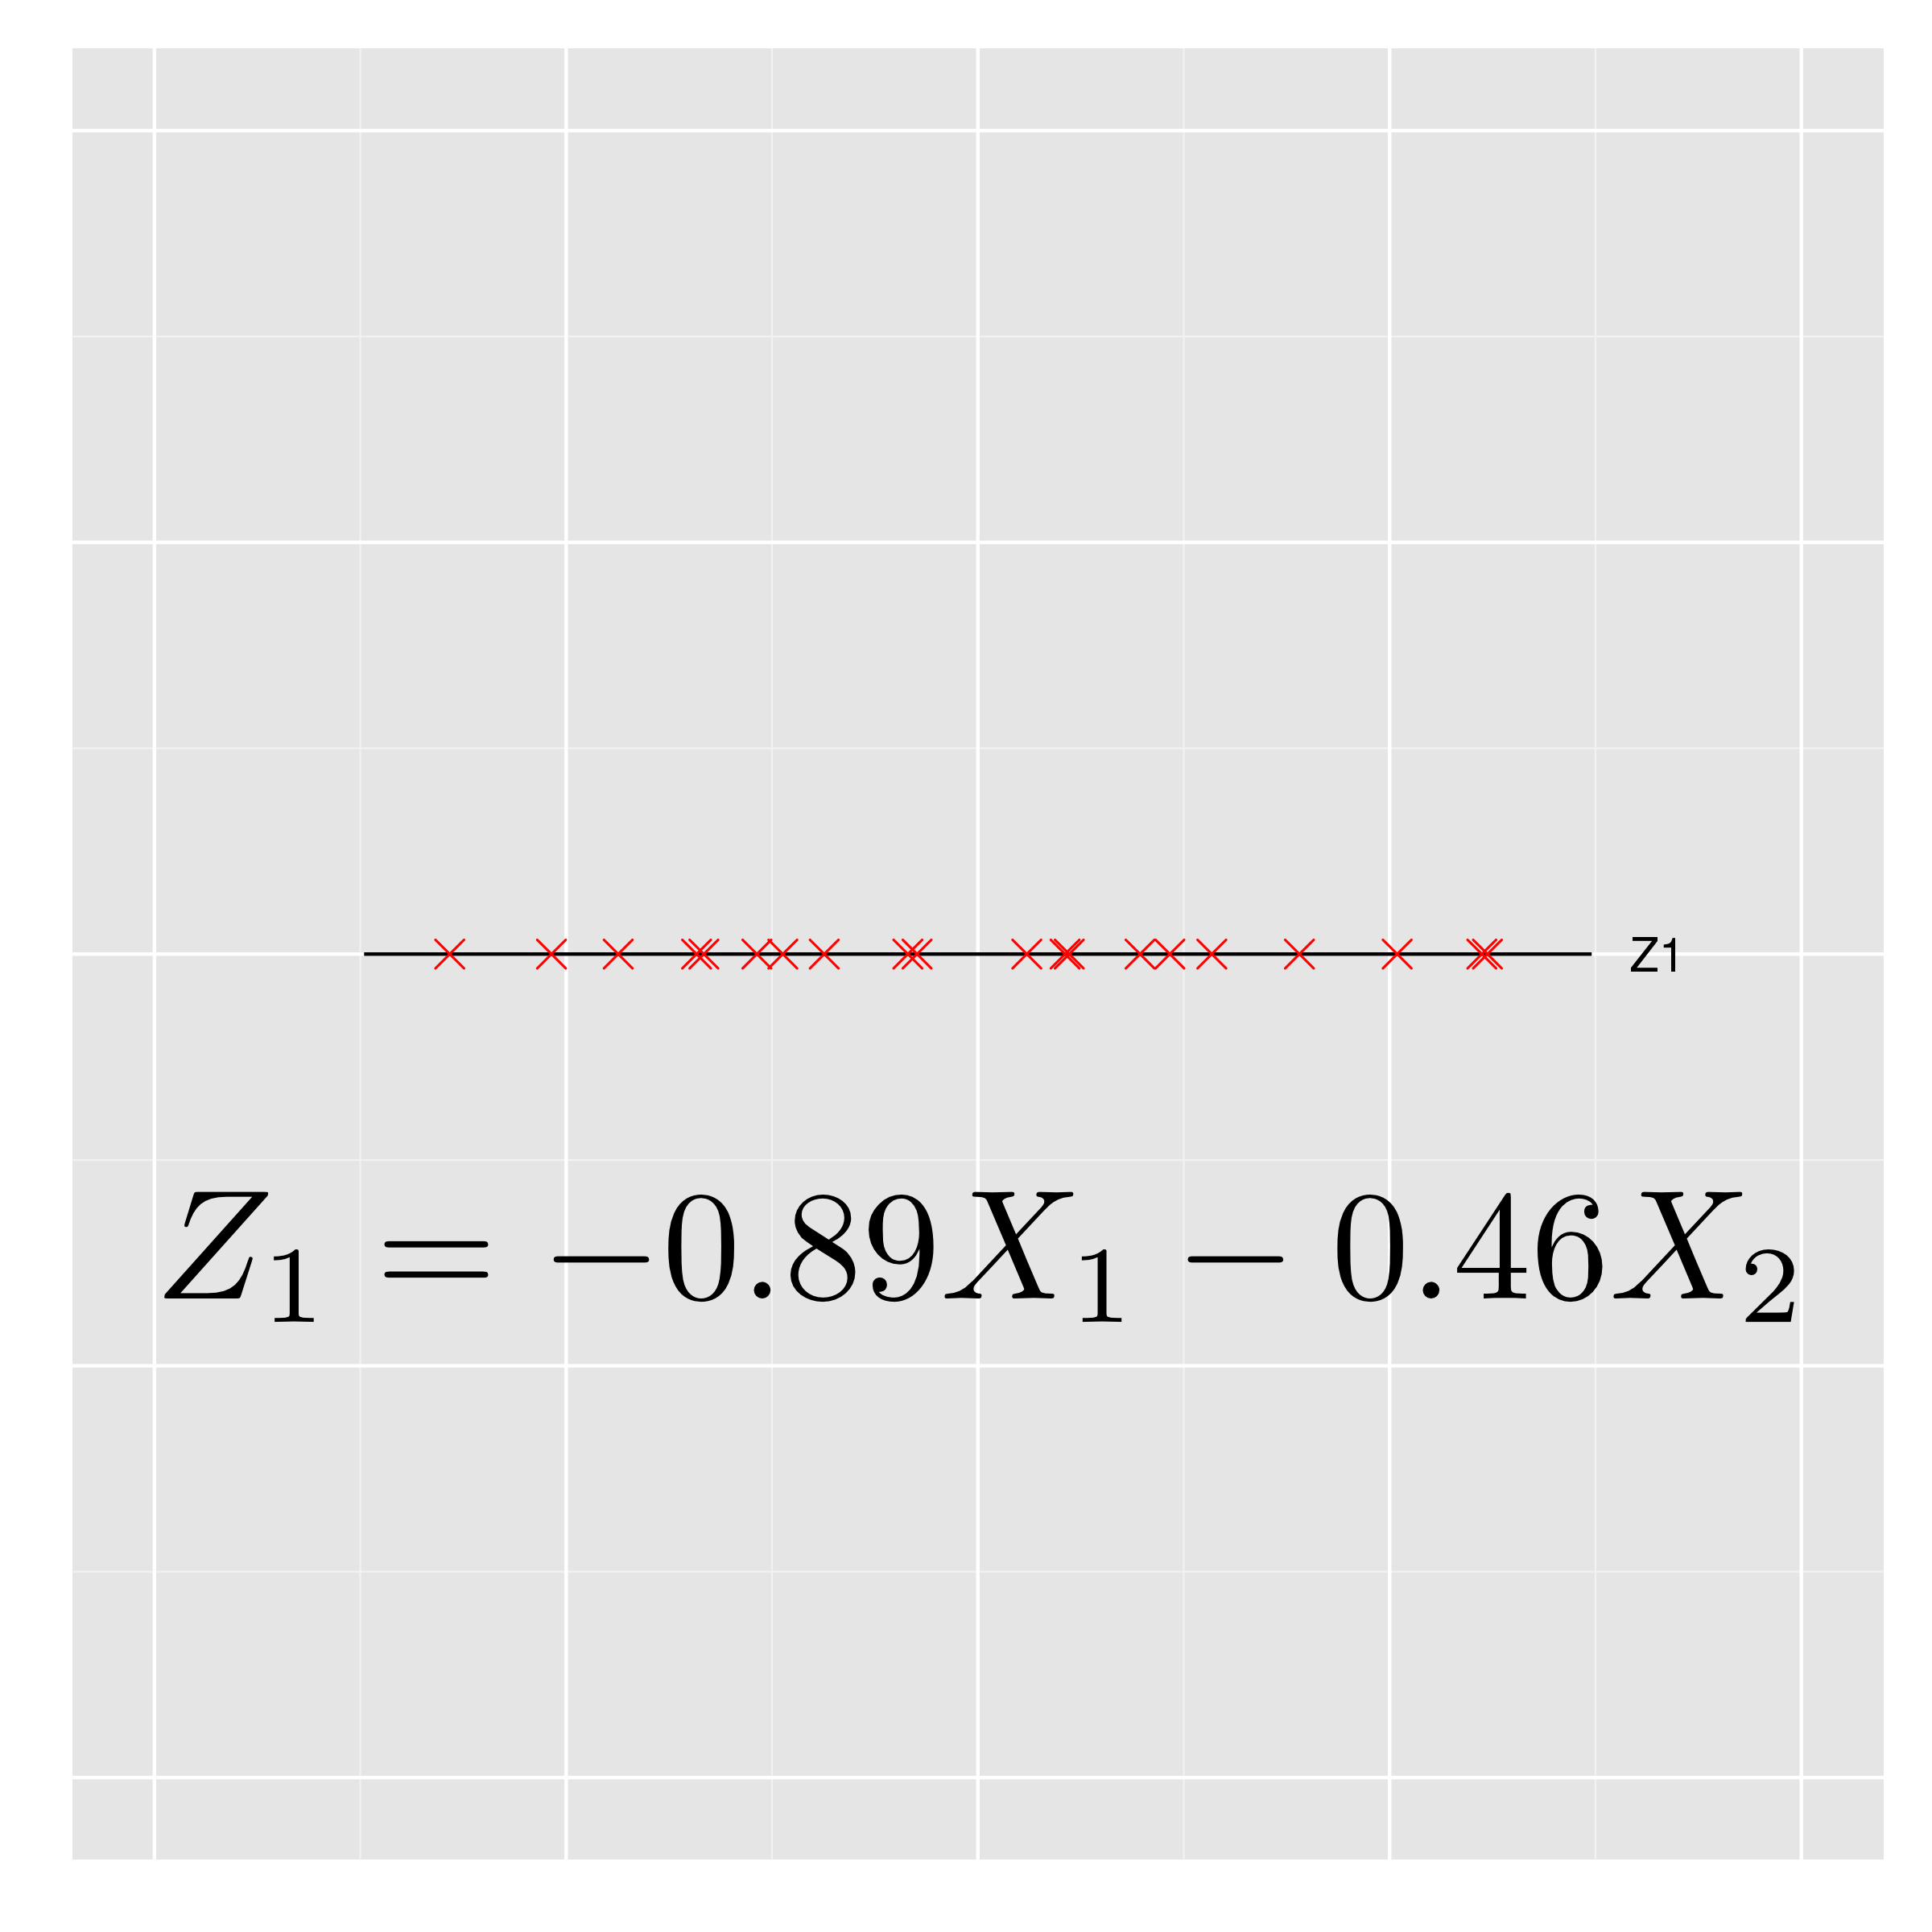
\includegraphics[height=7cm]{reduccion2d1d_expresion_z1.png}
 \end{center}
  \end{frame}

  \begin{frame}\frametitle{Propiedades fundamentales del ACP}
  Por la definición de los componentes principales, la matriz de covarianzas $S_Z$ es
$$S_Z=\left(\begin{array}{lllll}
\lambda_1&0&\ldots&\ldots&0\\
0&\lambda_2&0&\ldots&0\\
\vdots&\ldots&\ddots&\vdots&\vdots\\
0&\ldots&\ldots&\ldots&\lambda_k
\end{array}\right),$$
 Por lo tanto: 
 \begin{itemize}
 \item<+-> $\lambda_i=var(Z_i)$
 \item<+-> Los componentes principales son incorrelados ($r_{Z_iZ_j}=0$).
 \end{itemize}

  \end{frame}
\begin{frame}\frametitle{Propiedades fundamentales del ACP}
  Por teoremas de álgebra lineal:
  \begin{enumerate}
\item<+-> Cualquier combinación lineal estanderizada de las variables iniciales, es decir $a_1X_1+\cdots+a_kX_k$ con $a_1^2+\cdots+a_k^2=1$, presenta una varianza menor or igual que la del primer componente $Z_1$, es decir:
$$Var(a_1X_1+\cdots+a_kX_k)\leq \lambda_1.$$
  \begin{block}{Es decir:}
    Cuando fijamos el primer vector del nuevo sistema como $\vec{u_1}$, el vector propio de $S_X$ asociado a $\lambda_1$, maximizamos la varianza de los valores  que toma la primera componente en la nube de puntos
  \end{block}

\end{enumerate}
  \end{frame}
\begin{frame}\frametitle{Propiedades fundamentales del ACP}

\begin{enumerate}
  \setcounter{enumi}{1}
\item<+-> La variabilidad total se preserva.
\begin{eqnarray*}
Var(X_1)+\cdots+Var(X_k)&=&Var(Z_1)+\cdots+Var(Z_k)\\
&=&\lambda_1+\cdots+\lambda_k\\
\end{eqnarray*}
\end{enumerate}
\end{frame}
\begin{frame}\frametitle{¿Cómo escoger con cuántos componentes nos quedamos?}
                  \begin{overlayarea}{\textwidth}{6.5cm} 
  Nos basamos en la evolución de los valores propios: con dos opciones.
  \begin{enumerate}
  \item<+-> Diagrama de codo (Scree plot)
  \begin{center}
    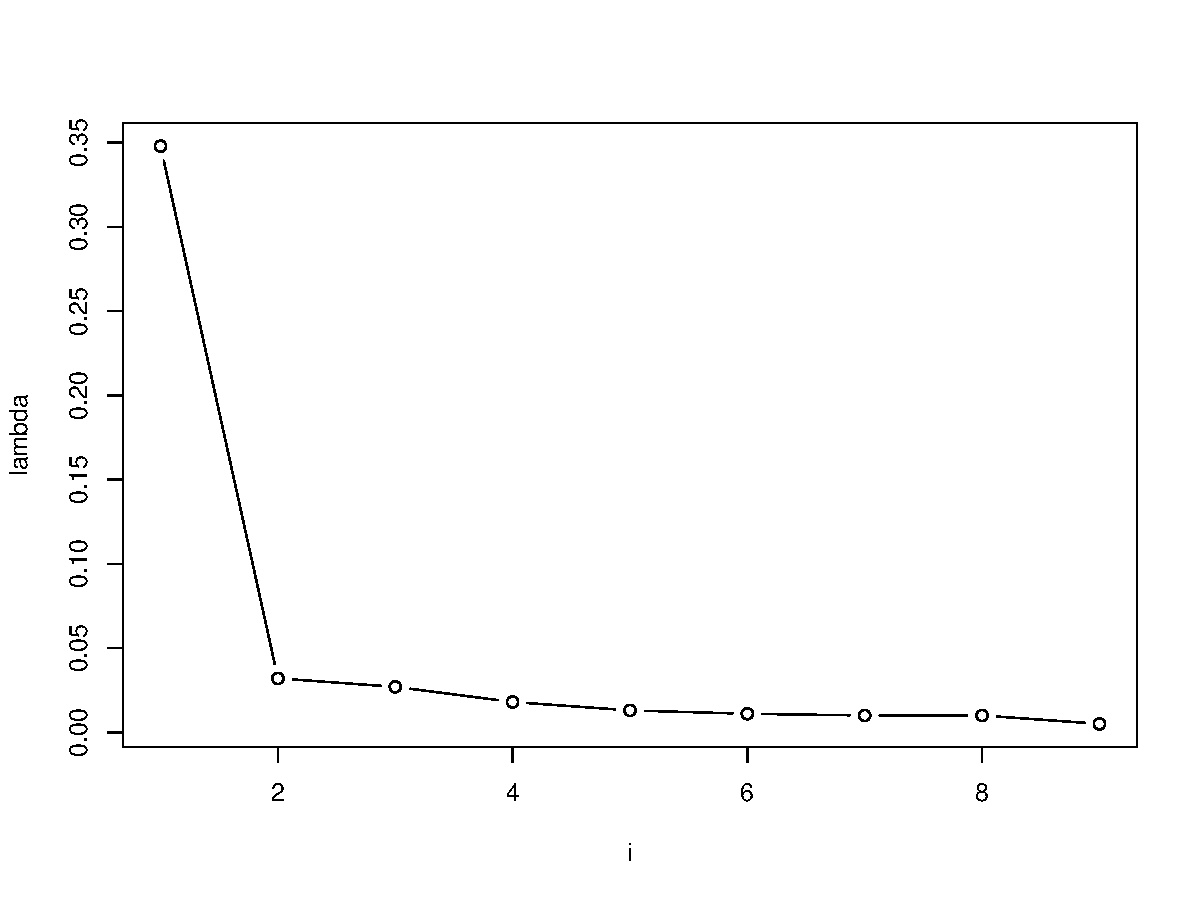
\includegraphics[width=5cm]{codoepf}
  \end{center}

  \end{enumerate}
                  \end{overlayarea}
  
\end{frame}
\begin{frame}\frametitle{¿Cómo escoger con cuántos componentes nos quedamos?}
              \begin{overlayarea}{\textwidth}{6.5cm} 
  Nos basamos en la evolución de los valores propios: con dos opciones.
  \begin{enumerate}
  \item<+-> Diagrama de codo (Scree plot)
  \begin{center}
    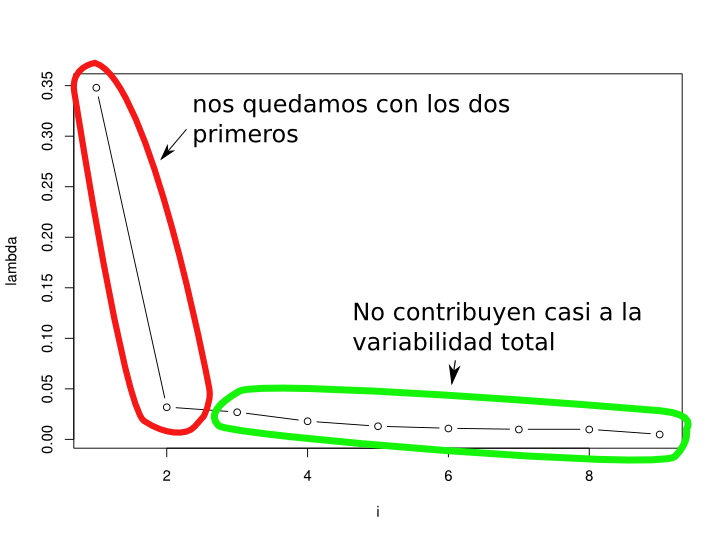
\includegraphics[width=5cm]{codo-texto.png}
  \end{center}

  \end{enumerate}
  
              \end{overlayarea}
\end{frame}

\begin{frame}\frametitle{¿Cómo escoger con cuántos componentes nos quedamos?}
                \begin{overlayarea}{\textwidth}{8cm} 
  Nos basamos en la evolución de los valores propios: con dos opciones.

  \begin{enumerate}
      \setcounter{enumi}{1}
  \item<+-> Varianza acumulada explicada. Ejemplo:
  \begin{center}
    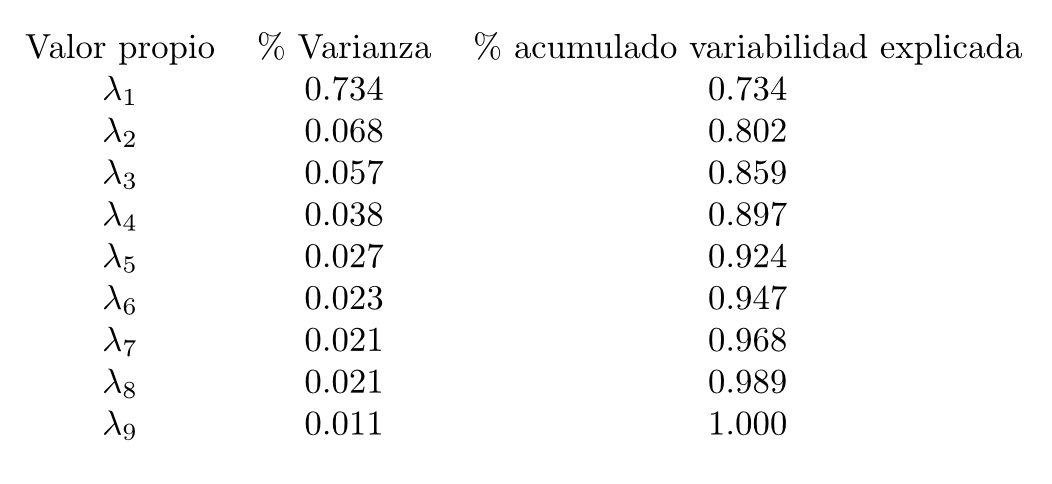
\includegraphics[width=8cm]{tabla-acp-crop.png}
  \end{center}

  \end{enumerate}
                \end{overlayarea}
  
\end{frame}

\begin{frame}\frametitle{¿Cómo escoger con cuántos componentes nos quedamos?}
                \begin{overlayarea}{\textwidth}{8cm} 
  Nos basamos en la evolución de los valores propios: con dos opciones.
  \begin{enumerate}  \setcounter{enumi}{1}
  \item<+-> Varianza acumulada explicada. Ejemplo:
  \begin{center}
    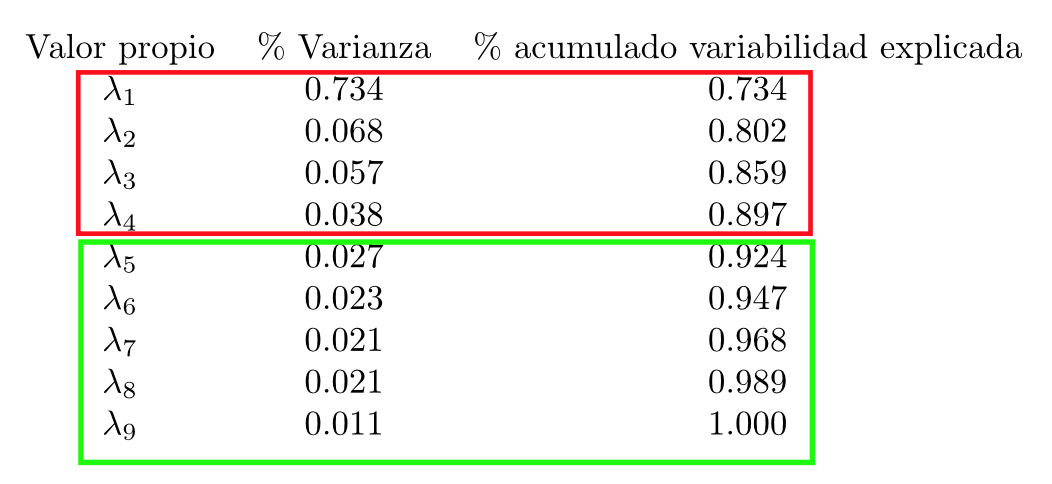
\includegraphics[width=8cm]{tabla-acp2-crop.png}
  \end{center}
\onslide<2-> Nos quedamos con los lambdas necesarios para alcanzar aprox. 90\% varianza.
  \end{enumerate}
                \end{overlayarea}
  
\end{frame}
\begin{frame}\frametitle{¿Cómo escoger con cuántos componentes nos quedamos?}
                \begin{overlayarea}{\textwidth}{8cm} 
  Nos basamos en la evolución de los valores propios: con dos opciones.
  \begin{enumerate}  \setcounter{enumi}{1}
  \item Varianza acumulada explicada. También se puede representar
    gráficamente la proporción acumulada de varianza explicada:
  \begin{center}
    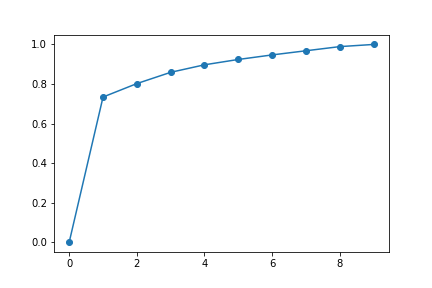
\includegraphics[width=8cm]{proporcion_acumulada_acp.png}
  \end{center}

  \end{enumerate}
                \end{overlayarea}
  
              \end{frame}

              \begin{pycode}
import numpy as np
from matplotlib import pyplot as plt
X = np.array([[ 1.00438605,  0.35937117],
       [-2.46602796, -1.06885082],
       [-2.80893108,  0.32134067],
       [ 2.88617809,  0.58024608],
       [ 1.67999909, -2.03154416],
       [ 4.9763785 ,  3.73233177],
       [ 5.76356187,  2.30991203],
       [ 4.03955618,  3.30669816],
       [ 1.02393382,  0.43324337],
       [-5.69224585, -2.95662229],
       [-3.37580554, -0.88656966],
       [-1.06494628,  0.22883757],
       [-0.95467755, -2.26251939],
       [ 1.86053646,  0.68297909],
       [ 1.48568532,  2.24178413],
       [-4.64199706, -0.48257437],
       [ 3.65015682,  1.43088013],
       [-0.43305149, -0.78558476],
       [-4.31356434, -2.9510243 ],
       [-2.61912501, -2.20233446]])
\end{pycode}
\begin{frame}[fragile]
  \frametitle{Análisis en componentes principales con {\tt
      scikit-learn}}
  Empezamos por cargar los datos del ejemplo:
  \begin{pyblock}
import pandas as pd
X = pd.read_csv('http://bit.ly/X_ejemplo_acp').values
\end{pyblock}
\onslide<2-> 
\begin{block}{}
    Usamos la clase {\tt PCA} del súbmodulo {\tt decomposition}.
    \begin{pyblock}
from sklearn.decomposition import PCA
    \end{pyblock}
    
  \end{block}\onslide<2->
  Podemos instanciar el transformador y  ajustarlo.
  \begin{pyblock}
acp = PCA()
acp.fit(X) # inplace
\end{pyblock}
\end{frame}
\begin{frame}[fragile]
Podemos ver la expresión de cada componente con el
atributo \pyv{components_}:
\begin{pyblock}
print(acp.components_)
\end{pyblock}
\begin{quote}
\printpythontex[verb]
\end{quote}
\onslide<2->
Cada componente es una línea de \pyv{acp.components_}, por lo tanto,
deducimos, redondeando

\begin{eqnarray*}
  Z_1&=&-0.89X_1-0.46X_2\\
Z_2&=&0.46X_1-0.89X_2\\
\end{eqnarray*}

\end{frame}


\begin{frame}[fragile]
Además, usando el atributo \pyv{explained_variance_} podemos obtener la varianza explicada por cada
componente, que coinciden con los auto-valores de $S_X$.

\onslide<2->
\begin{pyblock}
print(acp.explained_variance_)
\end{pyblock}
\begin{quote}
\printpythontex[verb]
\end{quote}
\onslide<3->
\begin{block}{}
  Podemos obtener la proporción de varianza explicada con el atributo \pyv{explained_variance_ratio_}
\begin{pyblock}
print(acp.explained_variance_ratio_)
\end{pyblock}
\begin{quote}
\printpythontex[verb]
\end{quote}
  
\end{block}


\end{frame}
\begin{frame}[fragile]
Ahora, podemos obtener las coordenadas de cada individuo en el nuevo
sistema de coordenadas, es decir los valores de cada individuo en los
componentes. Para ello, usamos el método \pyv{transform} aplicado a
nuestro transformador \pyv{acp}

\onslide<2->
\begin{pyblock}
Z = acp.transform(X)
\end{pyblock}

\onslide<3->
La matriz \pyv{Z} contiene las coordenadas de los puntos
en el nuevo sistema,
{\footnotesize
\begin{pyverbatim}
fig, ax = plt.subplots()
ax.scatter(Z[:,0], Z[:,1])
\end{pyverbatim}

\begin{center}
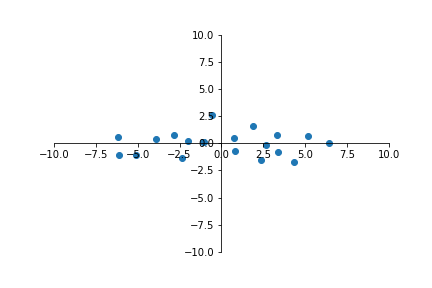
\includegraphics[width=6cm]{z1z2_matplotlib.png}
\end{center}
}
\end{frame}

\begin{frame}[fragile]
Por defecto la clase \pyv{PCA} conserva todos los componentes, pero
podríamos especificar directamente el número de componentes que
queremos conservar:
  \begin{pyblock}
acp1 = PCA(n_components=1)
acp1.fit(X) # inplace
Z1 = acp1.transform(X)
\end{pyblock}
\onslide<2-> \pyv{Z1} contiene ahora solo una columna, porque se ha
descartado la segunda componente. \onslide<3->
Lo representamos junto con \pyv{Z}:
{\footnotesize
\begin{pyverbatim}
fig, ax = plt.subplots()
ax.scatter(Z[:,0], Z[:,1])
ax.scatter(Z1, np.zeros(Z.shape[0]))
\end{pyverbatim}
}
\begin{center}
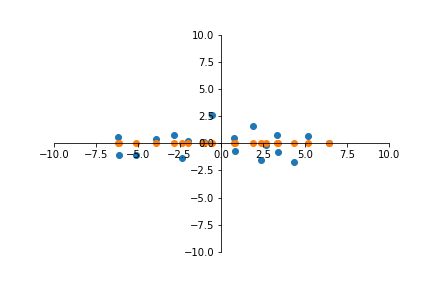
\includegraphics[width=6cm]{z1z2_reducido_matplotlib.png}
\end{center}
\end{frame}
\begin{frame}[fragile]
Finalmente, podríamos desde las coordenadas en el nuevo sistema,
volver a las coordenadas en el sistema original, usando el método \pyv{inverse_transform}
  \begin{pyblock}
X_reconstruido = acp.inverse_transform(Z)
X_reducido_reconstruido = acp1.inverse_transform(Z1)
\end{pyblock}
\onslide<2-> Si lo representamos
{\footnotesize
\begin{pyverbatim}
fig, ax = plt.subplots()
ax.scatter(X_reconstruida[:,0], X_reconstruida[:,1])
ax.scatter(X_reducida_recontruida[:,0], X_reducida_recontruida[:,1])
\end{pyverbatim}
}
\begin{center}
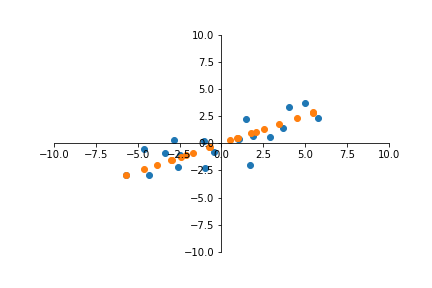
\includegraphics[width=6cm]{x1x2_reducido_matplotlib.png}
\end{center}
\end{frame}


\end{document}
